\chapter{The standard model and beyond}
\label{ch:theory}

Elementary particles and their interactions are described by a fundamental theory called standard model (SM)~\cite{QFTbook}.
It describes three of the four fundamental forces of nature, namely the electromagnetic, weak and strong interactions, in the form of quantum field theories (QFT) with local gauge invariance.
This theory has been confirmed by a large number of experimental results in the last forty years: from the precision measurements performed at the Large Electron Positron (LEP) and Tevatron~\cite{ALEPH:2010aa}
to the recent Large Hadron Collider (LHC) era (Chapter~\ref{ch:CMS}).
The SM constitutes one of the most successful achievements in modern physics.
It provides a very elegant theoretical framework, which is able to describe most of the known experimental phenomena in particle physics with high precision.

The basic ingredients of the SM are reviewed in Section~\ref{sec:SMintro}. This is followed by a discussion in Section~\ref{sec:SMLimitations} about few of the main open issues of the SM, which motivate theories of new physics.
Finally, three of the most popular theories beyond the standard model are introduced in Section~\ref{sec:BSMintro}. These models provide the theoretical framework, in which the search for new particles described in this thesis is conducted.
%As the work carried during this thesis is focused on a search for new heavy resonances, the last Section~\ref{sec:BSMintro} introduces some of the most popular theories of physics beyond the standard model (BSM).

%\section{The Standard Model}
  %%%%%%%%%%%%%%%%%%%%%%%%%%%%%%%%%%%%%%%%%%%%
\section{The standard model}\label{sec:SMintro}
%%%%%%%%%%%%%%%%%%%%%%%%%%%%%%%%%%%%%%%%%%%%

The standard model attempts to explain all the phenomena in nature in terms of the properties and interactions of a small number of fundamental particles
of three distinct categories (Table~\ref{tab:SMparticles}): two spin-1/2 families of fermions called \textit{leptons} and \textit{quarks}, and one family of spin-1 bosons called \textit{gauge bosons},
which act as `force carriers' in the theory.
All particles of the SM are assumed to be \textit{elementary}, i.e. they are treated as point particles, without internal structure or excited states.\\

\begin{table}[!htb]
\caption{Particles of the standard model~\cite{Olive:2016xmw}.}
\label{tab:SMparticles}
\begin{center}
\begin{tabular}{r | c | c | c | c | c |}
\cline{2-6}
                               & Symbol & Name  & Mass (\MeV) & Charge ($e$) & Spin\\
 \cline{2-6}
 Up-type quarks      & $u$ & up & 2.2 & +2/3 & 1/2\\
                               & $c$ & charm & 1.27 & +2/3 & 1/2\\
                               & $t$  & top & 173.21 & + 2/3 & 1/2\\
 \cline{2-6}
 Down-type quarks & $d$ & down & 4.7 & -1/3 & 1/2\\
                               & $s$ & strange & 96 & -1/3 & 1/2\\
                               & $b$ & bottom & 4.18 & -1/3 & 1/2\\
 \cline{2-6}
 Up-type leptons    & $\nu_e$ & electron neutrino & $< 2$ eV & 0 & 1/2\\
                              & $\nu_\mu$ & muon neutrino & $< 0.19$ & 0 & 1/2\\
                              & $\nu_\tau$ & tau neutrino & $< 18.2$ & 0 & 1/2\\
 \cline{2-6}
 Down-type leptons  & $e$ & electron & 0.51 & -1 & 1/2\\
                                 & $\mu$ & muon & 105.7 & -1 & 1/2\\
                                 & $\tau$ & tau & 1776.9 & -1 & 1/2\\
 \cline{2-6}   
 Gauge bosons & $\gamma$ & photon & 0 & 0 & 1\\
                         & $\PW^\pm$ & \PW & 80.4 \GeV & $\pm 1$ & 1\\
                         & \PZ & \PZ & 91.2 \GeV & 0 & 1\\ 
                         & $g$ & gluon & 0 & 0 & 1\\          
  \cline{2-6}   
  Higgs boson & \PH & Higgs & 125.1 \GeV & 0 & 0\\
  \cline{2-6}                                           
\end{tabular}
\end{center}
\end{table}

%fermion
The class of fermions include six quarks (up, down, charm, strange, top, bottom) and six leptons (electron, electron neutrino, muon, muon neutrino, tau, tau neutrino),
which are organized in three groups (generations) of pairs from each category:
%Pairs from each category are grouped together to form a generation, with corresponding particles exhibiting similar physical behavior.

\[
\begin{pmatrix}
  \nu_e & u \\ e & d
\end{pmatrix}
\qquad
,
\qquad
\begin{pmatrix}
  \nu_\mu & c \\ \mu & s
\end{pmatrix}
\qquad
,
\qquad
\begin{pmatrix}
  \nu_\tau & t \\ \tau & b
\end{pmatrix}.
\]

The defining property of the quarks is that they carry color charge, and hence, interact via the \textit{strong interaction}.
A phenomenon called color confinement results in quarks being very strongly bound to one another, forming color-neutral composite particles (\textit{hadrons})
containing either a quark and an antiquark (\textit{mesons}) or three quarks (\textit{baryons}).
Familiar examples of baryons are the proton and neutron, which also have the smallest mass among this family of particles.
As quarks also carry electric charge and weak isospin, they interact with other fermions both via the \textit{electromagnetic and weak interactions}.
The three neutrinos do not carry electric charge, so their interaction is only driven by the weak force, which makes them difficult to detect.
However, since they carry an electric charge, the electron, muon, and tau all interact electromagnetically.
Each member of a generation has greater mass than the corresponding particles of lower generations.
As the first generation charged particles do not decay, all ordinary matter is composed of such particles.
In particular, all atoms consist of electrons orbiting around atomic nuclei, ultimately constituted of up and down quarks.
Second and third generation charged particles, on the other hand, decay with very short half lives, and are observed only in very high-energy environments.
Neutrinos of all generations also do not decay, and pervade the universe, but rarely interact with ordinary matter.
Although neutrinos were originally assumed to be massless in the standard model, it is now known from experimental results that they have very small but finite masses.
To each of these fermions is associated an anti-particle with same mass and opposite quantum numbers.

In the SM, gauge bosons are defined as force carriers that mediate the strong, weak, and electromagnetic fundamental interactions.
The use of the word `gauge' refers to the fact that all three fundamental interactions arise as consequences of requiring invariance under local gauge symmetries. 
Specifically, the gauge symmetry group of the SM is $SU(3)_C \times SU(2)_L \times U(1)_Y$.
Among the gauge bosons, the \textit{photons} mediate the electromagnetic force between electrically charged particles.
The photon is massless and is well-described by the theory of \textit{quantum electrodynamics} (QED).
The $\PW^{\pm}$ and \PZ gauge bosons mediate the weak interactions between particles of different flavors (all quarks and leptons).
They are massive, with the \PZ being slightly heavier than the \PW.
The weak interactions involving the \PW exclusively act on left-handed particles and right-handed antiparticles.
Furthermore, the \PW carries an electric charge and couples to the electromagnetic interaction.
The electrically neutral \PZ boson interacts with both left-handed particles and antiparticles.
These three gauge bosons along with the photons are grouped together, as collectively mediating the \textit{electroweak interaction}, which is described in Section~\ref{subsec:EWtheory}.

Eight massless \textit{gluons} carrying color charge, mediate the strong interactions between quarks and also interact among themselves.
The gluons and their interactions are described by the theory of \textit{quantum chromodynamics} (QCD), which is described in Section~\ref{subsec:QCD}.

As discussed in more in detail in Section~\ref{subsec:EWSB}, one additional spin-0 particle, called the \textit{Higgs boson}, is postulated to explain the origin of mass within the theory,
since without it all the particles in the model are predicted to have zero mass.

%gravity
In addition to the strong, weak and electromagnetic interactions between quarks and leptons, there is a fourth force of nature, gravity, which is not accounted for in the standard model.
In fact, the gravitational interaction between elementary particles is so small that it can be neglected at the presently accessible energies.

%%%%%%%%%%%%%%%%%%%%%%%%%%%%%%%%%%%%%%%%%%%%
\subsection{Electroweak theory}\label{subsec:EWtheory}
%%%%%%%%%%%%%%%%%%%%%%%%%%%%%%%%%%%%%%%%%%%%

The theory of electroweak interactions is based on the $SU(2)_L \times U(1)_Y$ gauge group with the quantum numbers of weak isospin $I$ and hypercharge $Y$.
Quarks and leptons are represented by spinor fields $\psi$, which are functions of continuous space-time coordinates $x^\mu$.
From experimental evidences it is known that the weak interaction is of the form of vector minus axial current ($V - A$), or in other words, it couples only to left-handed chirality states.
It is therefore convenient to write the field $\psi$ as the sum of the two chirality components:

\begin{equation}\label{eqn:SM_e1}
\psi_L(x) = \frac{1-\gamma^5}{2}\psi(x) \qquad\qquad \mbox{and} \qquad\qquad  \psi_R(x) = \frac{1+\gamma^5}{2}\psi(x).
\end{equation}

The left-handed fields are grouped into $SU(2)_L$ doublets consisting of one charged and one neutral lepton, or one up and one down quark,
with a weak isospin $I = 1/2$:

\[
\begin{pmatrix}
  \nu_\ell \\ \ell
\end{pmatrix}_L
\qquad
\mbox{and}
\qquad
\begin{pmatrix}
  q_u \\ q_d 
\end{pmatrix}_L.
\]

For up-type quarks and neutrinos the third component of the weak isospin is assigned as $I_3 = +1/2$; for down-type quarks and charged leptons the component is $I_3 = -1/2$.
The right-handed partners ($\ell_R\, ,\, q_{uR}\, ,\, q_{dR}$) transform as $SU(2)_L$ singlet with weak isospin $I_3 = 0$.
The weak hypercharge $Y$ aforementioned is then defined via electric charge $Q$ and weak isospin to be $Y = 2Q - 2I_3$.
Thus, members within a doublet carry the same hypercharge: $Y = -1$ for leptons and $Y = 1/3$ for quarks.\\

In quantum field theories, the equations of motion for the different fields considered are derived from the Lagrangian that contains all the information on the fields and on their interaction.
In the SM, the fermionic fields are added by hand to the Lagrangian to account for experimental observations.
The situation is however different for the bosonic fields, as their existence is a direct consequence of invariance properties of the Lagrangian.
This mechanism can be understood by starting from the Lagrangian for a free spin-1/2 particle with mass $m$:

\begin{equation}\label{eqn:SM_e2}
\mathcal{L}_0 = i\bar{\psi}\gamma^\mu\partial_\mu\psi - m\bar{\psi}\psi , 
\end{equation}

\noindent where $\gamma^\mu$ are the Dirac matrices.
It is straightforward to verify that the $\mathcal{L}_0$ is invariant under \textit{global} $U(1)$ transformations

\begin{equation}\label{eqn:SM_e3}
\psi(x) \xrightarrow{U(1)} \psi^\prime(x) \equiv e^{iQ\theta} \psi(x),
\end{equation}

\noindent where $Q$ is the electric charge carried by the particle involved and $\theta$ an arbitrary constant.
However, the free Lagrangian is no longer invariant if one allows the phase transformation to depend on the space-time coordinate, i.e. under local phase redefinitions $\theta = \theta(x)$, because

\begin{equation}\label{eqn:SM_e4}
\partial_\mu\psi(x) \xrightarrow{U(1)} e^{iQ\theta} (\partial_\mu + iQ\partial_\mu\theta)\psi(x),
\end{equation}

\noindent and $\mathcal{L}_0$ picks up an extra term.
The \textit{gauge invariance} is the requirement that the $U(1)$ phase invariance should hold locally.
This is only possible if some additional terms are added to the Lagrangian, so to cancel the $\partial_\mu\theta$ term in Eq.~\ref{eqn:SM_e4}.
This is achieved by introducing a new spin-1 field $A_\mu(x)$, called a ``gauge'' field, that transforms as

\begin{equation}\label{eqn:SM_e5}
A_\mu(x) \xrightarrow{U(1)} A^\prime_\mu(x) \equiv A_\mu(x) + \frac{1}{e}\partial_\mu\theta, 
\end{equation}

\noindent and by defining a covariant derivative

\begin{equation}\label{eqn:SM_e6}
\mathcal{D}_\mu \equiv \partial_\mu - ieQA_\mu,
\end{equation}

\noindent which has the required property of transforming like the field itself:

\begin{equation}\label{eqn:SM_e7}
\mathcal{D}_\mu\psi(x) \xrightarrow{U(1)} (\mathcal{D}_\mu\psi)^\prime(x) \equiv e^{iQ\theta} \mathcal{D}_\mu\psi(x).
\end{equation}

The resulting Lagrangian

\begin{equation}\label{eqn:SM_e8}
\mathcal{L} = i\bar{\psi}\gamma^\mu\mathcal{D}_\mu\psi - m\bar{\psi}\psi = \mathcal{L}_0 + eQA_\mu\bar{\psi}\gamma^\mu\psi
\end{equation}

\noindent is then invariant under local $U(1)$ transformations.
For the new gauge field to be a true propagating field, a gauge-invariant kinetic term has to be added to the Lagrangian

\begin{equation}\label{eqn:SM_e9}
\mathcal{L}_A = -\frac{1}{4}F_{\mu\nu}F^{\mu\nu},
\end{equation}

\noindent where $F_{\mu\nu} \equiv \partial_\mu A_\nu - \partial_\nu A_\mu$. 
A possible mass term for the gauge field, $m^2A^\mu A_\mu$, is forbidden because it would violate gauge invariance,
so that it is predicted to be massless.
The new gauge field can be easily identified with the electromagnetic potential,
and the total Lagrangian 

\begin{equation}\label{eqn:SM_e10}
\mathcal{L} = \left[ i\bar{\psi}\gamma^\mu\partial_\mu\psi - m\bar{\psi}\psi \right] + \left[ -\frac{1}{4}F_{\mu\nu}F^{\mu\nu} \right] + [eQA_\mu\bar{\psi}\gamma^\mu\psi]
\end{equation}

\noindent gives rise to the well-known Maxwell equations of the electrodynamics

\begin{equation}\label{eqn:SM_e11}
\partial_\mu F^{\mu\nu} = J^\nu \, , \qquad\qquad J^\nu = -eQ\bar{\psi}\gamma^\nu\psi,
\end{equation}

\noindent where $J^\nu$ is the fermion electromagnetic current.
Thus, the final Lagrangian in Eq.~\ref{eqn:SM_e10} represents the final expression for the Lagrangian of quantum electrodynamics,
describing Dirac fields (fermions) interacting wth Maxwell fields (photons).\\

To describe weak interactions, a more elaborated structure is needed, with several fermionic flavors and different properties for left- and right-handed fields.
Moreover, the left-handed fermions must appear in doublets, and massive gauge bosons $\PW^{\pm}$ and $\PZ$ must be present in addition to the photon.
The simplest group with doublet representations is $SU(2)$, and since the theory must include QED as well, the additional $U(1)$ group is needed.
Hence, the obvious symmetry group to consider is $SU(2)_L \times U(1)_Y$, where $L$ refers to left-handed fields and $Y$ to the hypercharge.

The free Lagrangian for a generation of quarks (or leptons) is given by

\begin{equation}\label{eqn:SM_e12}
\mathcal{L}_0 = \sum_{j=1}^3 i\bar{\psi}_j\gamma^\mu\partial_\mu\psi_j,
\end{equation}

\noindent where the following notation has been introduced

\begin{equation}\label{eqn:SM_e13}
\psi_1(x) = 
\begin{pmatrix}
  u \\ d
\end{pmatrix}_L
\,
,
\qquad
\psi_2(x) = u_R \, , \qquad \psi_3(x) = d_R.
\end{equation}

The free Lagrangian $\mathcal{L}_0$ is invariant under global $G$ transformations in flavor space:

\begin{equation}\label{eqn:SM_e14}
\begin{split}
\psi_1(x) & \xrightarrow{G} \psi_1^\prime(x) \equiv e^{iY_1\beta}U_L\psi_1(x) \\ 
\psi_2(x) & \xrightarrow{G} \psi_2^\prime(x) \equiv e^{ig^\prime Y_2\beta}\psi_2(x) \\
\psi_3(x) & \xrightarrow{G} \psi_3^\prime(x) \equiv e^{ig^\prime Y_3\beta}\psi_3(x)
\end{split}
\end{equation}

\noindent where the $SU(2)_L$ transformation

\begin{equation}\label{eqn:SM_e15}
U_L \equiv e^{ig\frac{\tau^i}{2}\alpha^i} \qquad\qquad (i = 1,2,3)
\end{equation}

\noindent only acts on the doublet field $\psi_1$.
%The parameters $Y_i$ are the hypercharges, since the $\mathrm{U(1)_Y}$ phase transformation is analog to the QED one.
The parameters $Y_i$ are three different values (one per each field) of the hypercharge, which represents the generator of the symmetry group $U(1)_Y$.
The $\beta$ parameter is the phase of the $U(1)_Y$ transformation and is one-dimensional.
The matrices $\tau_i$ are the Pauli matrices and represent the three $SU(2)_L$ transformation generators which are combined in the weak isospin operator
$\textbf{T} = (\tau_1, \tau_2, \tau_3)$. These matrices form a Lie group, which is defined by the commutator relation $[\tau_i,\tau_j] = i\epsilon_{ijk}\tau_k$.
As the $\tau_i$ do not commute, the $SU(2)_L$ group is called non-Abelian.
%The matrix transformation UL is non-abelian.
Due to the generator structure, the phase $\alpha = (\alpha_1, \alpha_2, \alpha_3)$ of the $SU(2)_L$ transformation has to be extended to a three-component vector with the same dependencies as above.
The couplings $g$ and $g^\prime$ have been introduced for the $SU(2)_L$ and $U(1)_Y$, respectively, quantifying the strength of the interactions.

The free Lagrangian in Eq.~\ref{eqn:SM_e12} is then required to be invariant under local $SU(2)_L\times U(1)_Y$ gauge transformations,
i.e. with $\alpha_i = \alpha_i(x)$ and $\beta = \beta(x)$.
In order to satisfy this symmetry requirement, the fermion derivatives are exchanged with covariant objects.
Since there are now four gauge parameters, $\alpha_i(x)$ and $\beta(x)$, four different gauge fields are needed:

\begin{eqnarray}\label{eqn:SM_e16}
\mathcal{D}_\mu \equiv \partial_\mu + ig\textbf{W}_\mu \cdot \textbf{T} + ig^\prime\frac{Y}{2}B_\mu.
%\mathcal{D}_\mu \equiv \partial_\mu + ig\frac{\tau_i}{2}W^i_\mu + ig^\prime\frac{Y}{2}B_\mu.
\end{eqnarray}

Thus, four additional vector fields of spin 1 have been added: the isotriplet $\textbf{W}_\mu = (W_{1\mu}, W_{2\mu}, W_{3\mu})$ for the $SU(2)_L$ and the singlet $B_\mu$ for the $U(1)_Y$.
The quanta of these fields are called gauge bosons.
In order to build the gauge-invariant kinetic term for the gauge bosons, the corresponding field strengths are introduced: 

\begin{equation}\label{eqn:SM_e17}
\begin{split}
B_{\mu\nu} & \equiv \partial_\mu B_\nu - \partial_\nu B_\mu\\
W^i_{\mu\nu} & \equiv \partial_\mu W^\prime_\nu - \partial_\nu W^i_\mu - g\epsilon_{ijk} W^j_\mu W^k_\nu.
\end{split}
\end{equation}

The final $SU(2)_L \times U(1)_Y$ Lagrangian is then given by

\begin{equation}\label{eqn:SM_e18}
\mathcal{L}_{SU(2)_L\times U(1)_Y} = \mathcal{L}_f + \mathcal{L}_g,
\end{equation}

\noindent where $\mathcal{L}_f$ is the Lagrangian for the free fermion fields

\begin{equation}\label{eqn:SM_e19}
\mathcal{L}_f = i\sum_{j}\bar{\psi}^j_L\gamma^\mu[\partial_\mu + ig\textbf{W}_\mu \cdot \textbf{T} + ig^\prime\frac{Y_L}{2}B_\mu]\psi^i_L + i\sum_j\bar{\psi}^j_R[\partial_\mu - g^\prime Y_RB_\mu]\psi^j_R
\end{equation}

\noindent and $\mathcal{L}_g$ is the Lagrangian for the gauge bosons

\begin{equation}\label{eqn:SM_e20}
\mathcal{L}_g = -\frac{1}{4}\textbf{W}_{\mu\nu} \cdot \textbf{W}^{\mu\nu} - \frac{1}{4}B_{\mu\nu} \cdot B^{\mu\nu}.
\end{equation}

Since the field strengths $W^i_{\mu\nu}$ contain a quadratic term, the Lagrangian $\mathcal{L}_g$ gives rise to cubic and quartic self-interactions among the gauge fields.
The strength of these interactions is given by the same $SU(2)_L$ coupling $g$ which appears in the fermionic piece of the Lagrangian.
The final Lagrangian represents the unified electroweak theory, developed by Glashow~\cite{GLASHOW1961579}, Weinberg~\cite{PhysRevLett.19.1264} and Salam~\cite{RevModPhys.52.525}.
However, this is not the entire theory since the gauge symmetry forbids to write a mass term for the gauge bosons.
Fermionic masses are also not possible, because they would connect the left- and right-handed fields, which have different transformation properties, and therefore would produce an explicit breaking of the gauge symmetry.
Thus, the $SU(2)_L\times U(1)_Y$ Lagrangian in Eq.~\ref{eqn:SM_e17} only contains massless fields.
The mass terms are introduced through a procedure that exploits spontaneous symmetry breaking as described in the following.
%TF1* f = new TF1("f","-500*x*x+5*x*x*x*x",-15,15)
%TF1* f = new TF1("f","x*x",-10,10)
%TF3* f3 = new TF3("f3","x*x+y*y-z",-10,10,-10,10,0,1000)
%TF3* f3 = new TF3("f3","-500*(x*x+y*y)+5*(x*x+y*y)^2-z",-10,10,-10,10,-15000,0)

%%%%%%%%%%
\subsection{Spontaneous symmetry breaking}\label{subsec:EWSB}
%%%%%%%%%%

In order to generate masses, the gauge symmetry needs to be broken in such way to maintain the full symmetry of the Lagrangian.
The main idea is based on the possibility to obtain non-symmetric results from a Lagrangian that possess the following properties:
it is invariant under a group $G$ of transformations and has a degenerate set of states with minimal energy, which transform under $G$ as the members of a given multiplet.
As it will be demonstrated in the following, by arbitrary selecting one of those states as the ground state of the system, one says that the symmetry becomes spontaneously broken.
%The idea is that the lowest energy (vacuum) state does not respect the gauge symmetry and induces effective masses for particles propagating through it.

In order to explain this mechanism the Lagrangian for a complex scalar field $\phi(x) = \phi_1(x) + i\phi_2(x)$ is considered

\begin{equation}\label{eqn:SM_e21}
\mathcal{L} = \partial_\mu\phi^\dag\partial^\mu\phi - V(\phi) \, , \qquad\qquad V(\phi) = \mu^2\phi^\dag\phi + h(\phi^\dag\phi)^2
\end{equation}

\noindent where $V(\phi)$ is a potential. 
The Lagrangian $\mathcal{L}$ is invariant under global phase transformations of the scalar field

\begin{equation}\label{eqn:SM_e22}
\phi(x) \xrightarrow{U(1)} \phi^\prime(x) \equiv e^{i\theta} \phi(x).
\end{equation}

In order to allow for a minimum or ``ground state'' of the potential, the parameter $h$ has to be $\geq 0$. For the quadratic term there are the two following possibilities.
If $\mu^2 \geq 0$, the potential acquires only the trivial minimum $\phi_m = 0$. If $\mu^2 \leq 0$ the minimum is obtained for all those field configurations satisfying

\begin{equation}\label{eqn:SM_e23}
|\phi_m| = \sqrt{\frac{-\mu^2}{2h}} \equiv \frac{v}{\sqrt{2}} \geq 0 \qquad\qquad \Rightarrow \qquad\qquad V(\phi_m) = -\frac{h}{4}v^4
\end{equation}

As the Lagrangian is invariant under $U(1)$ phase transformations, there is an infinite number of degenerate states of minimum energy given by 
$\phi_m(x) = \frac{v}{\sqrt{2}}e^{i\theta}$.
A particular solution can be chosen, e.g. $\theta = 0$, corresponding to the minimum of the field given by $\phi_{1m} = v/\sqrt{2}$ and $\phi_{2m} = 0$.
Since the Feynman calculus is a perturbation procedure, in which starting from a ground state the fields are treated as fluctuations about that state,
two new real fields $\eta(x)$ and $\xi(x)$ are introduced representing these fluctuations

\begin{equation}\label{eqn:SM_e24}
\eta(x) = \phi_1(x) - \frac{v}{\sqrt{2}} \qquad\qquad \mbox{and} \qquad\qquad \xi(x) = \phi_2(x).
\end{equation}

In terms of these new fields, the potential $V(\phi)$ takes the form

\begin{equation}\label{eqn:SM_e25}
V(\phi) = V(\phi_m) - \mu^2\eta^2 + hv\eta(\eta^2+\xi^2) + \frac{h}{4}(\eta^2+\xi^2)^2
\end{equation}

\noindent and the resulting Lagrangian does not share the same symmetry of the original one. Thus, by choosing a particular solution as the ground state, the symmetry gets spontaneously broken.
At the same time, the second term of the potential in Eq.~\ref{eqn:SM_e25} is a mass term, so the real field $\eta$ describes a massive state of mass $m_\eta = -2\mu^2$.
The second real field $\xi$ is massless, and its appearance can be understood as follows.
The field $\xi$ describes excitations around a flat direction in the potential, i.e. into states with the same energy as the chosen ground state.
Since those excitations do not cost any energy, they correspond to a massless state.
The fact that there are massless excitations associated with the spontaneous symmetry breaking mechanism is a general result, known as the \textit{Goldstone theorem}:
if a Lagrangian is invariant under a continuous symmetry group $G$, but the vacuum is only invariant under a subgroup $H \subset G$,
then there must exist as many massless spin-0 particles (\textit{Goldstone bosons}) as broken generators (i.e. generators of $G$ which do not belong to $H$).\\

%%%%%%%%%%%%%%%%%%%%%%%%%%%%%%%%%%%%%%
\subsection{The Higgs mechanism}\label{subsec:HiggsMech}
%%%%%%%%%%%%%%%%%%%%%%%%%%%%%%%%%%%%%%

The mechanism of spontaneous symmetry breaking described in the previous section does not account for the mass of the gauge fields of the weak interaction,
since it introduces an additional massless scalar boson that is not included in the set of the known elementary particles.
However, further elements are added to the theory  when applying the idea of spontaneous symmetry breaking to the case of local gauge invariance.
In order to achieve this, the complex scalar field $\phi(x)$ introduced in the previous section is replaced with a $SU(2)_L$ doublet of complex scalar fields with $U(1)$ hypercharge $Y = +1/2$:

\begin{equation}\label{eqn:SM_e26}
\phi(x) \equiv
\begin{pmatrix}
  \phi^+(x) \\ \phi^0(x)
\end{pmatrix}
= \frac{1}{\sqrt{2}}
\begin{pmatrix}
  \phi_1(x) - i\phi_2(x) \\ \phi_3(x) - i\phi_4(x)
\end{pmatrix}.
\end{equation}

The gauged scalar Lagrangian of the Goldstone model (Eq.~\ref{eqn:SM_e21}) is now given by

\begin{equation}\label{eqn:SM_e27}
\begin{aligned}
\mathcal{L}_\phi  & = \mathcal{D}_\mu\phi^\dag\mathcal{D}^\mu\phi - \mu^2\phi^\dag\phi + h(\phi^\dag\phi)^2 \, , & \qquad (h \geq 0, \mu^2 \leq 0) \, , \\
 \mathcal{D}^\mu\phi & =  [\partial^\mu + ig\textbf{W}_\mu \cdot \textbf{T} + ig^\prime\frac{Y}{2}B_\mu] \, , & \qquad (Y = Q - \tau_3 = \frac{1}{2}) \, , 
\end{aligned}
\end{equation}

\noindent and it is invariant under local $SU(2)_L \times U(1)_Y$ transformations.
The value of the scalar hypercharge is fixed by the requirement of having the correct couplings between $\phi(x)$ and $B_\mu(x)$, i.e. that the photon does not couple to $\phi^0$, and one has the right electric charge for $\phi^+$.
As observed in the previous section, there is an infinite set of degenerate states with minimum energy satisfying

\begin{equation}\label{eqn:SM_e29}
\begin{aligned}
\left\langle0|\phi_i|0\right\rangle & = 0 \quad \mbox{for} \quad i = 1,2,4\\
\left\langle0|\phi_3|0\right\rangle & = \sqrt{\frac{-\mu^2}{2h}} \equiv \frac{v}{\sqrt{2}}.
\end{aligned}
\end{equation}

Since the electric charge is a conserved quantity, only the neutral scalar field can acquire a vacuum expectation value.
Once a particular ground state is chosen, the $SU(2)_L\times U(1)_Y$ symmetry gets spontaneously broken.
%to the electromagnetic subgroup $\mathrm{U(1)_{QED}}$, which by construction still remains a true symmetry of the vacuum. According to Goldstone theorem 3 massless states should then appear.
On the other hand, the vacuum carries no electric charge, so the $U(1)_{Q}$ of QED is not broken.
Thus, the $SU(2)_L\times U(1)_Y$ group of the electroweak theory is spontaneously broken to the $U(1)_{Q}$ subgroup, i.e. $SU(2)_L \times U(1)_Y \rightarrow U(1)_Q$.

The scalar doublet can now be written in its general, gauge-invariant form as a fluctuation over the ground state

\begin{equation}\label{eqn:SM_e30}
\phi(x) = e^{i\frac{\tau^i}{2}\theta^i(x)}\frac{1}{\sqrt{2}}
\begin{pmatrix}
  0 \\ v + H(x)
\end{pmatrix}
\end{equation}

\noindent with 4 real fields $\theta^i(x)$ and $H(x)$.
The crucial point is that the local $SU(2)_L$ invariance of the Lagrangian allows one to rotate away any dependence on $\theta^i(x)$.
These three fields would be precisely the massless Goldstone bosons associated with the spontaneous symmetry breaking mechanism.
The additional ingredient of gauge symmetry makes these massless excitations unphysical.
%The covariant derivative in Eq.~\ref{eqn:SM_e28} couples the scalar multiplet to the $\mathrm{SU(2)_L\times U(1)_Y}$ gauge bosons.
In fact, it can be demonstrated that by choosing the physical (unitary) gauge $\theta^i(x) = 0$, the 3 massless Goldstone bosons
arising from the three broken generators can be eliminated from the Lagrangian.
At the same time, the kinetic piece of the scalar Lagrangian in Eq.~\ref{eqn:SM_e27} takes the form

\begin{equation}\label{eqn:SM_e31}
(\mathcal{D}_\mu\phi)^\dag\mathcal{D}^\mu\phi \xrightarrow{\theta^i = 0} \frac{1}{2}\partial_\mu H\partial^\mu H + (v+H)^2 \left\{ \frac{g^2}{4}W^\dag_\mu W^\mu + \frac{g^2}{8\cos^2\theta_W}Z_\mu Z^\mu \right\}.
\end{equation}

The vacuum expectation value of the neutral scalar has generated a quadratic term, i.e. mass terms, for the gauge bosons.
Usually, one rewrites the fields in terms of the three massive vector bosons $\PW^\pm$ and \PZ, and a massless vector boson, the photon $A$.
One finds that they are mixtures of the original gauge fields $\mathbf{W}_\mu$ and $B_\mu$:

\begin{equation}\label{eqn:SM_e32}
W^\pm_\mu = \frac{(W^1_\mu \mp iW^2_\mu)}{\sqrt{2}},
\end{equation}

\begin{equation}\label{eqn:SM_e33}
\begin{pmatrix}
  A_\mu \\ Z_\mu
\end{pmatrix}
=
\begin{pmatrix}
  \cos\theta_W & \sin\theta_W \\ -\sin\theta_W & \cos\theta_W
\end{pmatrix}
\begin{pmatrix}
  B_\mu \\ W^3_\mu
\end{pmatrix}
\end{equation}

\noindent where the Weinberg angle $\theta_W$ is defined as the ratio of coupling constants: $\tan\theta_W \equiv g^\prime/g$.
The masses of the gauge bosons $\PW^\pm$ and the \PZ are then given by:

\begin{equation}\label{eqn:SM_e34}
M_\PW = \frac{1}{2}vg \qquad\qquad \mbox{and} \qquad\qquad M_\PZ = \frac{v\sqrt{g^2 + g^{\prime 2}}}{2} = \frac{M_\PW}{\cos\theta_W}.
\end{equation}

The Lagrangian $\mathcal{L}_\phi$ has to be added to the electroweak theory given by the Lagrangian of Eqs.~\ref{eqn:SM_e18}--\ref{eqn:SM_e20}, such that

\begin{equation}\label{eqn:SM_e35}
\mathcal{L}_{SU(2)_L \times U(1)_Y} = \mathcal{L}_f + \mathcal{L}_g + \mathcal{L}_\phi.
\end{equation}

The total Lagrangian is invariant under gauge transformations, which guarantees the renormalizability of the associated quantum field theory.
After spontaneous symmetry breaking, three massless Goldstone bosons are generated, however, they are then eliminated from the Lagrangian by exploiting local gauge symmetry.
Going to the unitary gauge, the $\PW^\pm$ and the \PZ (but not the photon, because $U(1)_Q$ is an unbroken symmetry) have acquired masses given by Eq.~\ref{eqn:SM_e34}.
%Notice that (3.22) has now the meaning of writing the gauge fields in terms of the physical boson fields with definite mass.
In fact, before the spontaneous symmetry breaking mechanism, the massless $\PW^\pm$ and \PZ bosons lead to $3\times2 = 6$ degrees of freedom (d.o.f.), due to the two possible polarizations of a massless spin-1 field.
The four real scalar fields are also present at this stage, corresponding to additional four d.o.f.
After spontaneous symmetry breaking, the three Goldstone modes are ``eaten'' by the weak gauge bosons, which become massive, and therefore acquire one additional longitudinal polarization.
This leads to a total of $3 \times 3 = 9$ d.o.f. in the gauge sector, plus the remaining scalar particle $H$, which is called the \textit{Higgs boson}. The total number of d.o.f. is obviously conserved.
This theory is generally called the \textit{Higgs mechanism} and it was proposed by three independent groups in 1964: by Brout and Englert~\cite{PhysRevLett.13.321}, by Higgs~\cite{Higgs1964132,PhysRevLett.13.508,PhysRev.145.1156}, and by Guralnik, Hagen, and Kibble~\cite{PhysRevLett.13.585}.

The W and Z were discovered at CERN by the UA1~\cite{ARNISON1986484} and UA2~\cite{ANSARI1987440} groups in 1983.
Subsequent measurements of their masses and other properties at Tevatron and LEP have been in excellent agreement with the standard model expectations~\cite{Schael:2013ita,Aaltonen:2013iut}. The current values are $M_\PW = 80.385 \pm 0.015\GeV$ and $M_\PZ = 91.1876 \pm 0.0021\GeV$~\cite{Olive:2016xmw}.

%%%%%%%%%%%%%%%%%%%%%%%%%%%%%%%%%%%%%%
\subsection{The Higgs and Yukawa interactions}\label{subsec:HiggsBoson}
%%%%%%%%%%%%%%%%%%%%%%%%%%%%%%%%%%%%%%

The scalar Lagrangian in Eq.~\ref{eqn:SM_e27} has introduced a new scalar particle into the model: the Higgs boson H.
In terms of the physical fields (unitary gauge), $\mathcal{L}_\phi$ takes the form

\begin{equation}\label{eqn:SM_e36}
\mathcal{L}_\phi = \frac{1}{4}hv^4 + \mathcal{L}_H + \mathcal{L}_{HG^2}, 
\end{equation}

\noindent where

\begin{equation}\label{eqn:SM_e37}
\begin{gathered}
\mathcal{L}_H = \frac{1}{2}\partial_\mu H\partial^\mu H - \frac{1}{2}M^2_HH^2 -\frac{M^2_H}{2v}H^3 -\frac{M^2_H}{8v^2}H^4 \, , \\
\mathcal{L}_{HG^2} = M^2_WW^\dag_\mu W^\mu \left\{ 1 + \frac{2}{v}H + \frac{H^2}{v^2} \right\} + \frac{1}{2}M^2_ZZ_\mu Z^\mu \left\{ 1 + \frac{2}{v}H + \frac{H^2}{v^2} \right\} \, ,
\end{gathered}
\end{equation}

\noindent and the Higgs boson mass is given by

\begin{equation}\label{eqn:SM_e38}
M_H = \sqrt{-2\mu^2} = \sqrt{2h}v.
\end{equation}
 
A fermionic mass term $-m\bar{\psi}\psi$ is not allowed, because it breaks the gauge symmetry.
%However, since an additional scalar doublet has been added into the model, one can write the following gauge-invariant fermion-scalar couplings:
However, by adding Yukawa interaction terms of the fermion and Higgs field to the Lagrangian, the fermion masses can also be generated by spontaneous symmetry breaking.
This procedure is briefly described in the following.
%Similarly, this applies for quarks. 

The most general Yukawa Lagrangian can be written in the form

\begin{equation}\label{eqn:SM_e39}
\sum_{jk}\left\{
(\bar{u}^\prime_j , \bar{d}^\prime_j)_L
\left[
c^{(d)}_{jk}
\begin{pmatrix}
  \phi^+ \\ \phi^0
\end{pmatrix}
d^\prime_{kR} + c^{(u)}_{jk}
\begin{pmatrix}
  \phi^{0*} \\ -\phi^-
\end{pmatrix}
u^\prime_{kR}
\right]
+ (\bar{\nu}^\prime_j , \bar{\ell}^\prime_j) c^{(\ell)}_{jk}
\begin{pmatrix}
  \phi^+ \\ \phi^0
\end{pmatrix}
\ell^\prime_{kR}
\right\} + h.c.
\end{equation}

\noindent where the indexes run over the three generations of fermions;
$u^\prime_j$, $d^\prime_j$, $\ell^\prime_j$ and $\nu^\prime_j$ denote the weak eigenstates for the members of each generation $j$,
and $c^{(d)}_{jk}$, $c^{(u)}_{jk}$, and $c^{(\ell)}_{jk}$ are the so-called Yukawa couplings.
%$u^\prime$ and $d^\prime$ denote up- and down-type quarks, respectively,
%$\ell = e,\mu,\tau$, and $c^{(d)}_{jk}$, $c^{(u)}_{jk}$, and $c^{(\ell)}_{jk}$ are arbitrary coupling constants.
After spontaneous symmetry breaking, the Yukawa Lagrangian in the unitary gauge takes the simpler form

\begin{equation}\label{eqn:SM_e40}
\mathcal{L}_Y = - (1+\frac{H}{v})\{ \bar{\mathbf{d}}^\prime_L \mathbf{M}^\prime_d \mathbf{d}^\prime_R +  \bar{\mathbf{u}}^\prime_L \mathbf{M}^\prime_u \mathbf{u}^\prime_R\}
+ \bar{\mathbf{l}}^\prime_L \mathbf{M}^\prime_\ell \mathbf{l}^\prime_R + h.c. ,
\end{equation}

\noindent where $\bar{\mathbf{d}}^\prime$, $\bar{\mathbf{u}}^\prime$ and $\bar{\mathbf{l}}^\prime$ denote vectors in the 3-dimensional generation space, and the corresponding mass matrices are given by

\begin{equation}\label{eqn:SM_e41}
(\mathbf{M}^\prime_d)_{ij} \equiv -c^{(d)}_{ij}\frac{v}{\sqrt{2}} \, , \qquad (\mathbf{M}^\prime_u)_{ij} \equiv -c^{(u)}_{ij}\frac{v}{\sqrt{2}} \, , \qquad (\mathbf{M}^\prime_\ell)_{ij} \equiv -c^{(\ell)}_{ij}\frac{v}{\sqrt{2}}.
\end{equation}

Therefore, the spontaneous symmetry breaking mechanism generates fermion masses, which in turn fix all Yukawa couplings.
In general the mass matrices in Eq.~\ref{eqn:SM_e41} are not diagonal, Hermitian, or symmetric.
Thus, to identify the physical mass eigenstates $d_j$, $u_j$, and $\ell_j$, which are linear combinations of the corresponding weak eigenstates $d^\prime_j$, $u^\prime_j$, and $\ell^\prime_j$, it is necessary to diagonalize the matrices by separate unitary transformations on the left- and right-handed fermion fields. This is achieved as follows.
%The diagonalization of the mass matrices in Eq.~\ref{eqn:SM_e41} determines the mass eigenstates $d_j$, $u_j$, and $\ell_j$, which are linear combinations of the corresponding weak eigenstates $d^\prime_j$, $u^\prime_j$, and $\ell^\prime_j$, respectively.
The matrix $\mathbf{M}^\prime_d$ can be decomposed as $\mathbf{M}^\prime_d = \mathbf{H}_d\mathbf{U}_d = \mathbf{S}^\dag_d\mathcal{M}_d\mathbf{S}_d\mathbf{U}_d$,
where $\mathbf{H}_d \equiv \sqrt{\mathbf{M}^\prime_d\mathbf{M}^{\prime\dag}_d}$ is an hermitian positive-definite matrix, while $\mathbf{U}_d$ is unitary.
The $\mathbf{H}_d$ matrix can be diagonalized by a unitary matrix $\mathbf{S}_d$; the resulting matrix $\mathcal{M}_d$ is diagonal, hermitian and positive definite.
Similarly, one has $\mathbf{M}^\prime_u = \mathbf{H}_u\mathbf{U}_u = \mathbf{S}^\dag_u\mathcal{M}_u\mathbf{S}_u\mathbf{U}_u$.
In terms of the diagonal mass matrices

\begin{equation}\label{eqn:SM_e42}
\mathcal{M}_d = \mathrm{diag}(m_d, m_s, m_b) \, , \quad \mathcal{M}_u = \mathrm{diag}(m_u, m_c, m_t) \, , \quad \mathcal{M}_\ell = \mathrm{diag}(m_e, m_\mu, m_\tau)
\end{equation}

\noindent the Yukawa Lagrangian takes the simpler form

\begin{equation}\label{eqn:SM_e43}
\mathcal{L}_Y = - (1 + \frac{H}{v}) \{ \bar{\mathbf{d}}\mathcal{M}_d\mathbf{d} + \bar{\mathbf{u}}\mathcal{M}_u\mathbf{u}  + \bar{\mathbf{l}}\mathcal{M}_\ell\mathbf{l} \}
\end{equation}

\noindent where the mass eigenstates are defined by

\begin{equation}\label{eqn:SM_e44}
\begin{aligned}
\mathbf{d}_L  & \equiv \mathbf{S}_d\mathbf{d}^\prime_L  \, ,                     & \mathbf{u}_L  & \equiv \mathbf{S}_u\mathbf{u}^\prime_L \, ,                       & \mathbf{l}_L & \equiv \mathbf{S}_\ell\mathbf{l}^\prime_L \, , \\
\mathbf{d}_R & \equiv \mathbf{S}_d\mathbf{U}_d\mathbf{d}^\prime_R \, , & \mathbf{u}_R & \equiv \mathbf{S}_u\mathbf{U}_u\mathbf{u}^\prime_R \, ,  & \mathbf{l}_R & \equiv \mathbf{S}_\ell\mathbf{U}_\ell\mathbf{l}^\prime_R \, , \\
\end{aligned}
\end{equation}

One observes that the Higgs interactions (Fig.~\ref{fig:HiggsSM}) have a very characteristic form: they are always proportional to the squared mass of the coupled boson or fermion.
All Higgs couplings are therefore determined by $M_\PH$, $M_\PW$, $M_\PZ$, the mass $m_f$ of fermions, and the vacuum expectation value $v$.

\begin{figure}[!htb]
\centering
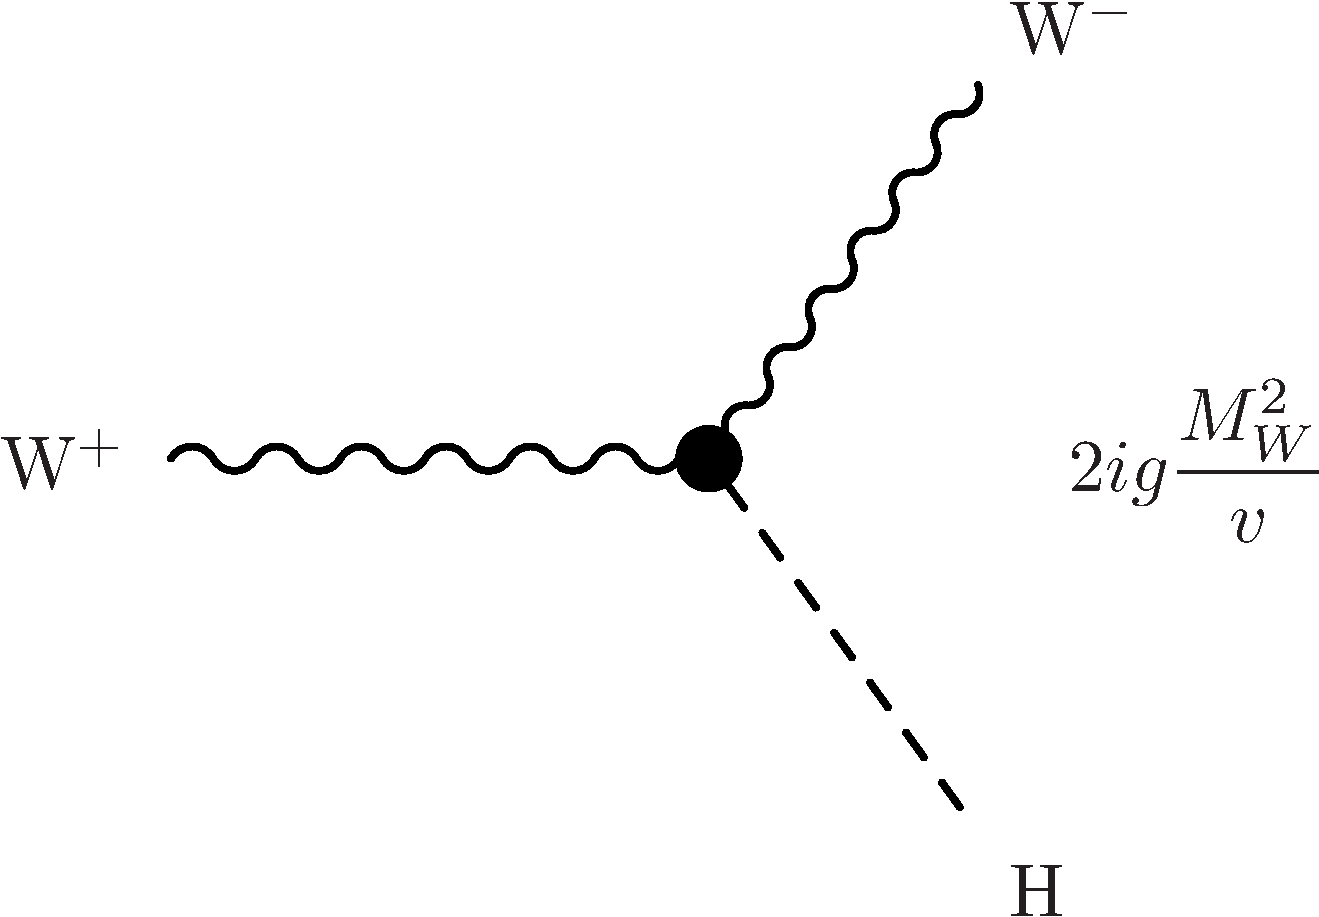
\includegraphics[width=0.3\textwidth]{\chtwo/Higgs_WWH_2.pdf}\hspace{0.4cm}
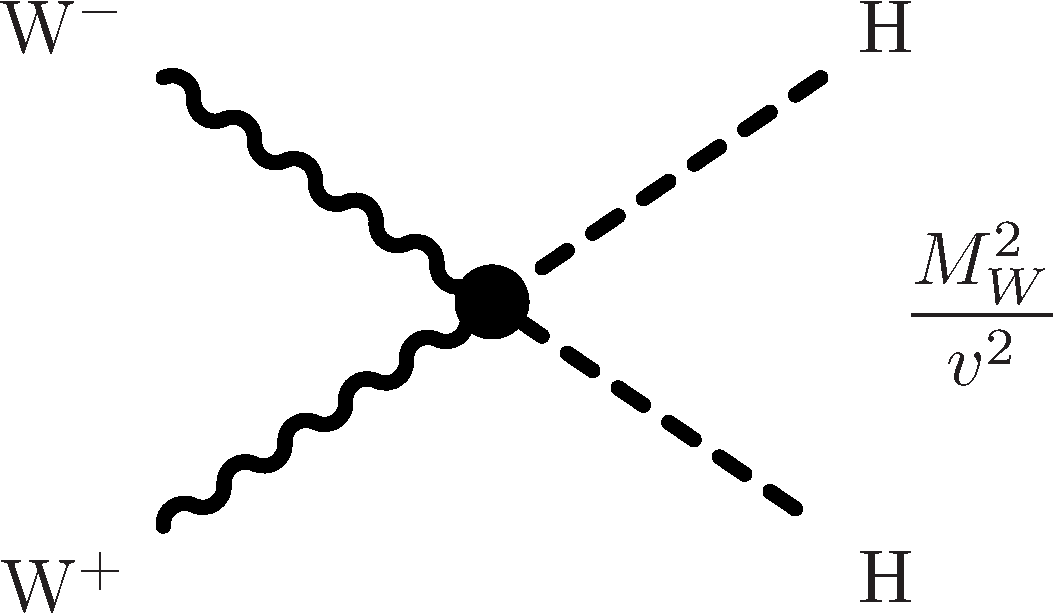
\includegraphics[width=0.3\textwidth]{\chtwo/Higgs_WWHH.pdf}\hspace{0.4cm}
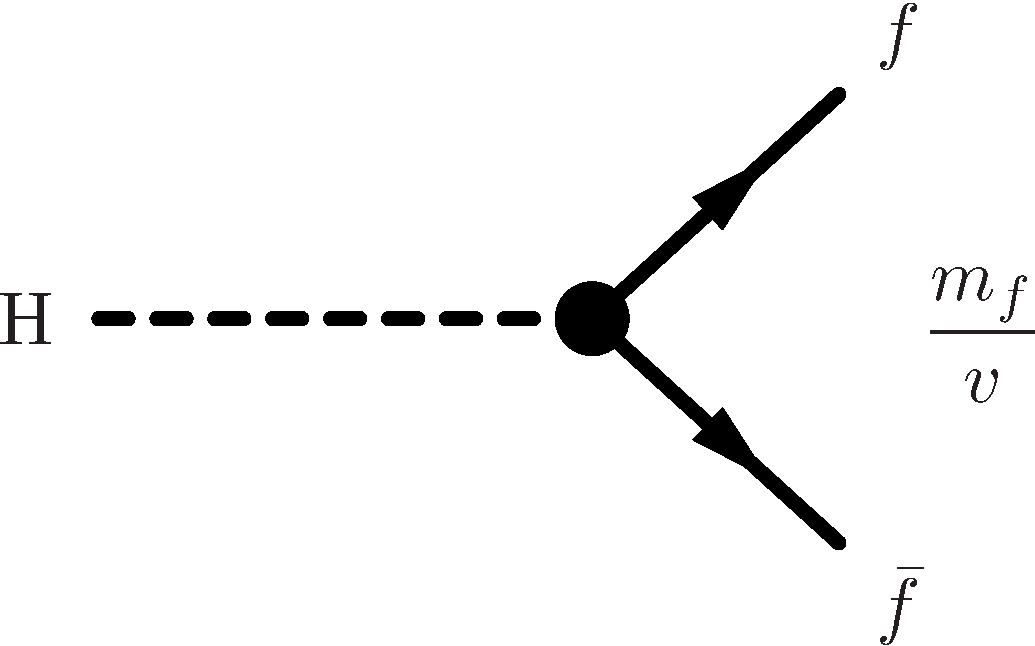
\includegraphics[width=0.3\textwidth]{\chtwo/Higgs_ffH.pdf}\\ \vspace{0.4cm}
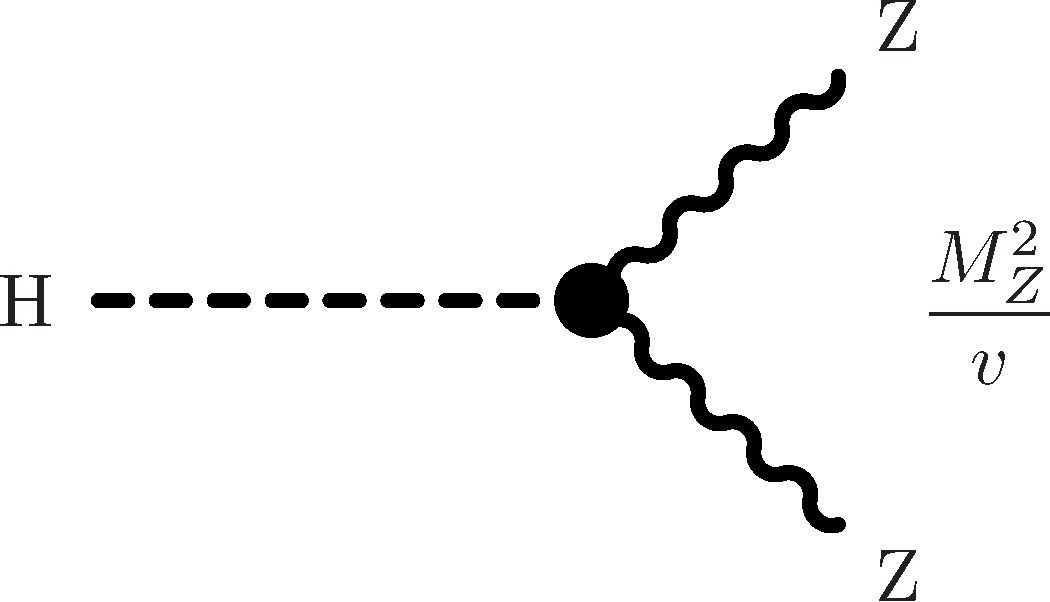
\includegraphics[width=0.3\textwidth]{\chtwo/Higgs_ZZH_2.pdf}\hspace{0.4cm}
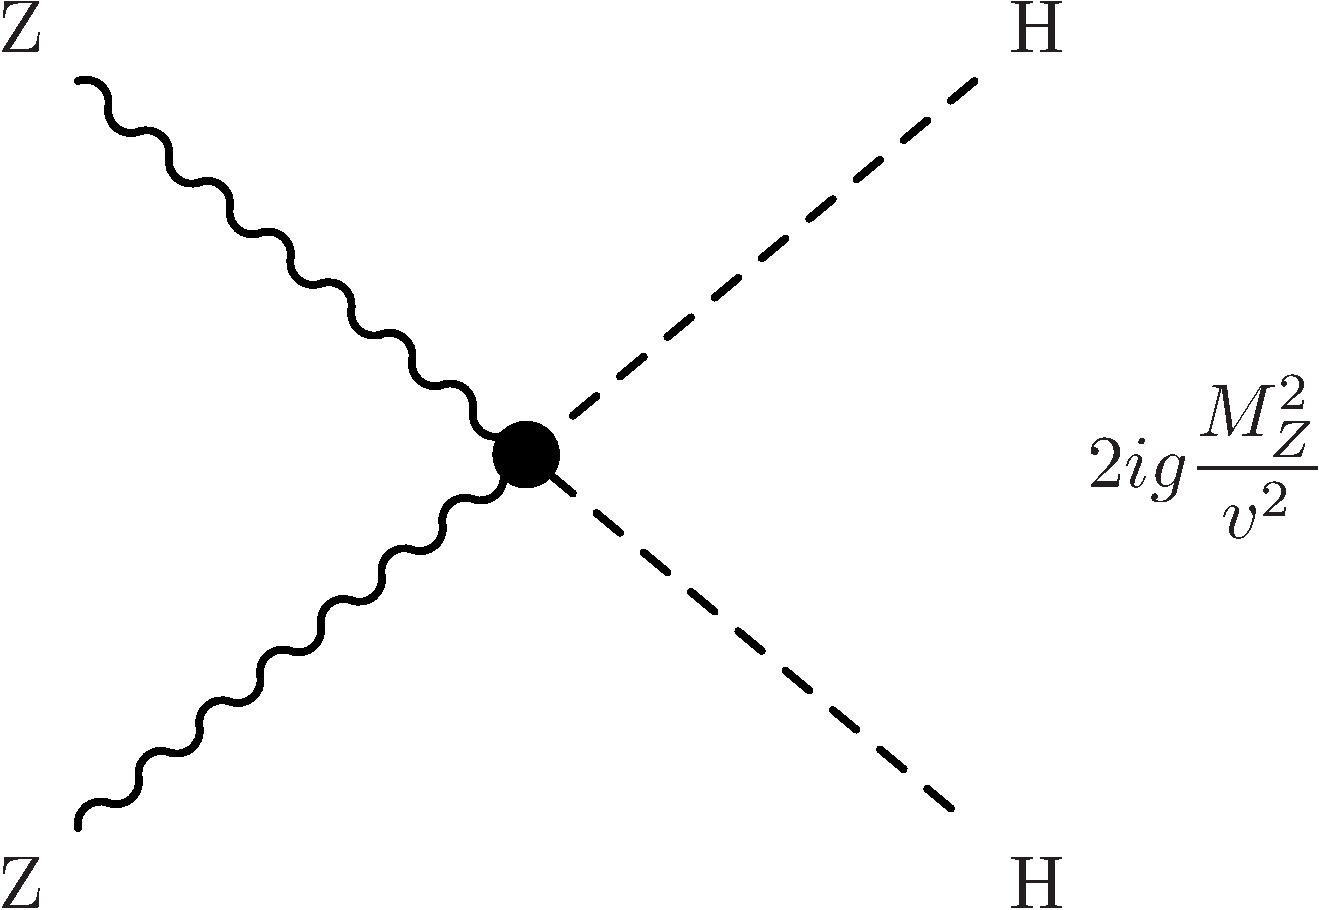
\includegraphics[width=0.3\textwidth]{\chtwo/Higgs_ZZHH.pdf}

\includegraphics[width=0.3\textwidth]{\chtwo/blank.png}\\ \vspace{0.4cm}
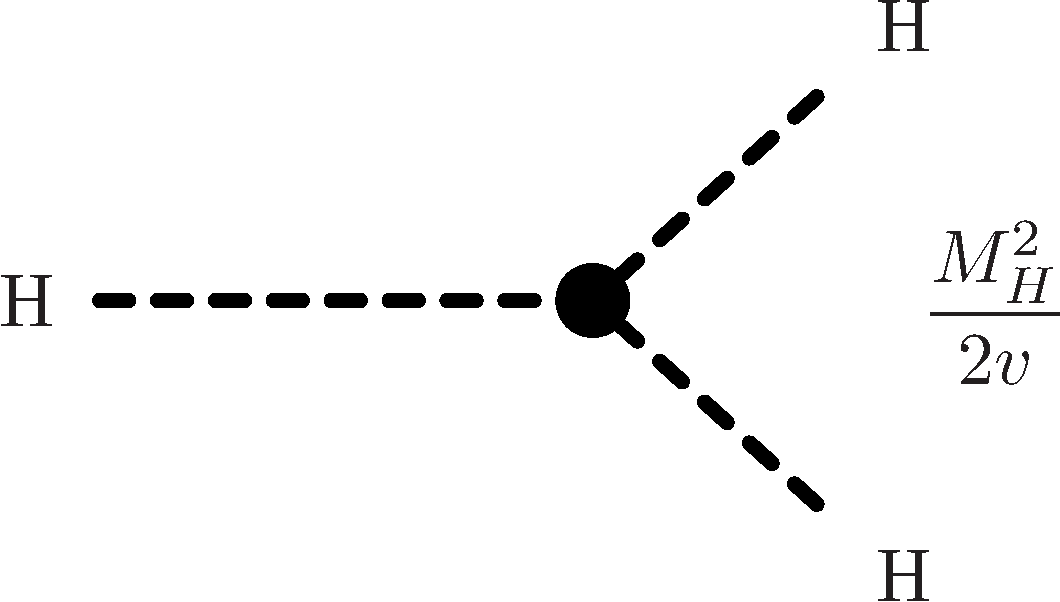
\includegraphics[width=0.3\textwidth]{\chtwo/Higgs_HHH.pdf}\hspace{0.4cm}
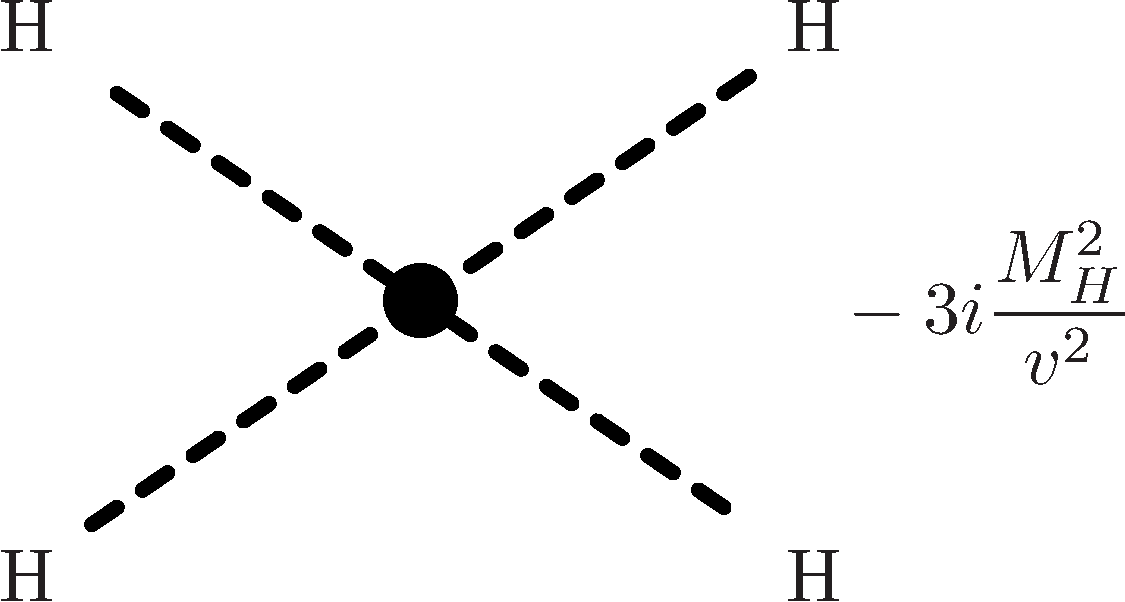
\includegraphics[width=0.3\textwidth]{\chtwo/Higgs_HHHH.pdf}

\includegraphics[width=0.3\textwidth]{\chtwo/blank.png}\\
\caption{Higgs interaction vertices in the standard model.}
\label{fig:HiggsSM}
\end{figure}

%Since, $\bar{\mathbf{f}}^\prime_L\mathbf{f}^\prime_L = \mathbf{f}_L\mathbf{f}_L$ and $\bar{\mathbf{f}}^\prime_R\mathbf{f}^\prime_R = \mathbf{f}_R\mathbf{f}_R$ ($f = u, d, \ell$),
%the form of the neutral-current part of the $\mathrm{SU(2)_L\times U(1)_Y}$ Lagrangian does not change when expressed in terms of mass eigenstates.
%Therefore, there are no flavor-changing neutral currents in the SM. %(GIM mechanism [4]).
%This is a consequence of treating all equal-charge fermions on the same footing.
%However, $\bar{\mathbf{u}}^\prime_L\mathbf{d}^\prime_L = \bar{\mathbf{u}}_L\mathbf{S}_u\mathbf{S}^\dag_d\mathbf{d}_L \equiv \bar{\mathbf{u}}_L\mathbf{V}\mathbf{d}_L$.
%In general, $\mathbf{S}_u \neq \mathbf{S}_d$; thus if one writes the weak eigenstates in terms of mass eigenstates, a $3\times3$ unitary mixing matrix $\mathbf{V}$, called the Cabibbo-Kobayashi-Maskawa (CKM) matrix\cite{CKM}, appears in the quark charged-current sector and couples any up-type quark with all down-type quarks:
%
%\begin{equation}\label{eqn:SM_e45}
%\begin{pmatrix}
%d^\prime \\ s^\prime \\ b^\prime
%\end{pmatrix}
%= \mathbf{V}
%\begin{pmatrix}
%d \\ s \\ b
%\end{pmatrix}_L
%=
%\begin{pmatrix}
%V_{ud} & V_{us} & V_{ub}\\
%V_{cd} & V_{cs} & V_{cb}\\
%V_{td} & V_{ts} & V_{tb}
%\end{pmatrix}
%\begin{pmatrix}
%d \\ s \\ b
%\end{pmatrix}_L
%\end{equation}
%
%The absolute values of its entries can be measured independently, but most precisely determined by a global fit that uses all available measurements.
%Requiring three generations of quarks and unitarity of the matrix yields the following absolute values~\cite{Olive:2016xmw,Hocker:2001xe,Charles2005}:
%
%\begin{equation}\label{eqn:SM_e46}
%\begin{pmatrix}
%0.97434^{+0.00011}_{-0.00012} & 0.22506 \pm 0.00050 & 0.00357 \pm 0.00015\\
%0.22492 \pm 0.00050                 & 0.97351 \pm 0.00013 & 0.0411 \pm 0.0013\\
%0.00875^{+0.00032}_{-0.00033} & 0.0403 \pm 0.0013    & 0.99915 \pm 0.00005
%\end{pmatrix}
%\end{equation}
%
%One observes large couplings close to 1 within the same generation (diagonal entries) whereas the off-diagonal entries are significantly smaller.
%With three quark generations, the unitarity requirement and taking into account that the quark phases cannot be measured the number of independent parameters of the matrix is reduced to four: three mixing angles between the quark generations and one complex phase that accounts for CP violation. Analogously, there exists a matrix describing the leptonic mixing, the Pontecorvo-Maki-Nakagawa-Sakata (PMNS) matrix~\cite{Ziro,PONTECORVO1968630}. It also contains four independent parameters if one assumes that neutrinos are not Majorana particles.

%%%%%%%%%%%%%%%%%%%%%%%%%%%%%%%%%%%%%%
\subsection{Observation of a particle compatible with the standard model Higgs boson}\label{subsec:HiggsLHC}
%%%%%%%%%%%%%%%%%%%%%%%%%%%%%%%%%%%%%%

The SM Higgs boson production cross sections at a proton-proton collider is shown in Fig.~\ref{fig:HiggsXS_a} as a function of the Higgs mass hypothesis and for the different leading production mechanisms.
In addition, in Fig.~\ref{fig:HiggsProd}, the corresponding Leading Order (LO) Feynman diagrams are shown.
Gluon fusion process ($gg \to \PH$) is the dominating Higgs production mechanism over the entire mass range accessible at the LHC.
In the vector boson fusion process  ($\mathrm{qq}^\prime \to \mathrm{qq}^\prime \PH$), which is about one order of magnitude weaker than gluon fusion, the Higgs boson is produced through a direct coupling with vector bosons (\PW or \PZ), which are irradiated by a pair of incoming quarks from the proton beams. 
The associated production with a \PW or \PZ boson ($\mathrm{q\bar{q}}^\prime \to \PW\PH$, $\qqbar \to \PZ\PH$) have a smaller cross section than the previous mechanisms but, the presence of the vector boson helps in reconstructing the events reducing the contamination from other SM processes.
The associated production with \ttbar pairs (qq, $gg \to \ttbar\PH$) has the smallest cross section, however, it allows for a direct access to the Higgs coupling to top quarks, representing thus an important process.
Depending on the Higgs boson mass hypothesis, different decay channels (Fig.~\ref{fig:HiggsXS_b}) can be exploited to detect it.
The Higgs boson does not couple to photons and gluons at LO, but such processes can arise via fermion or vector boson loops, giving a sizable contribution in the low mass region.\\

\begin{figure}[!htb]
\centering
\subfigure[]{\label{fig:HiggsXS_a}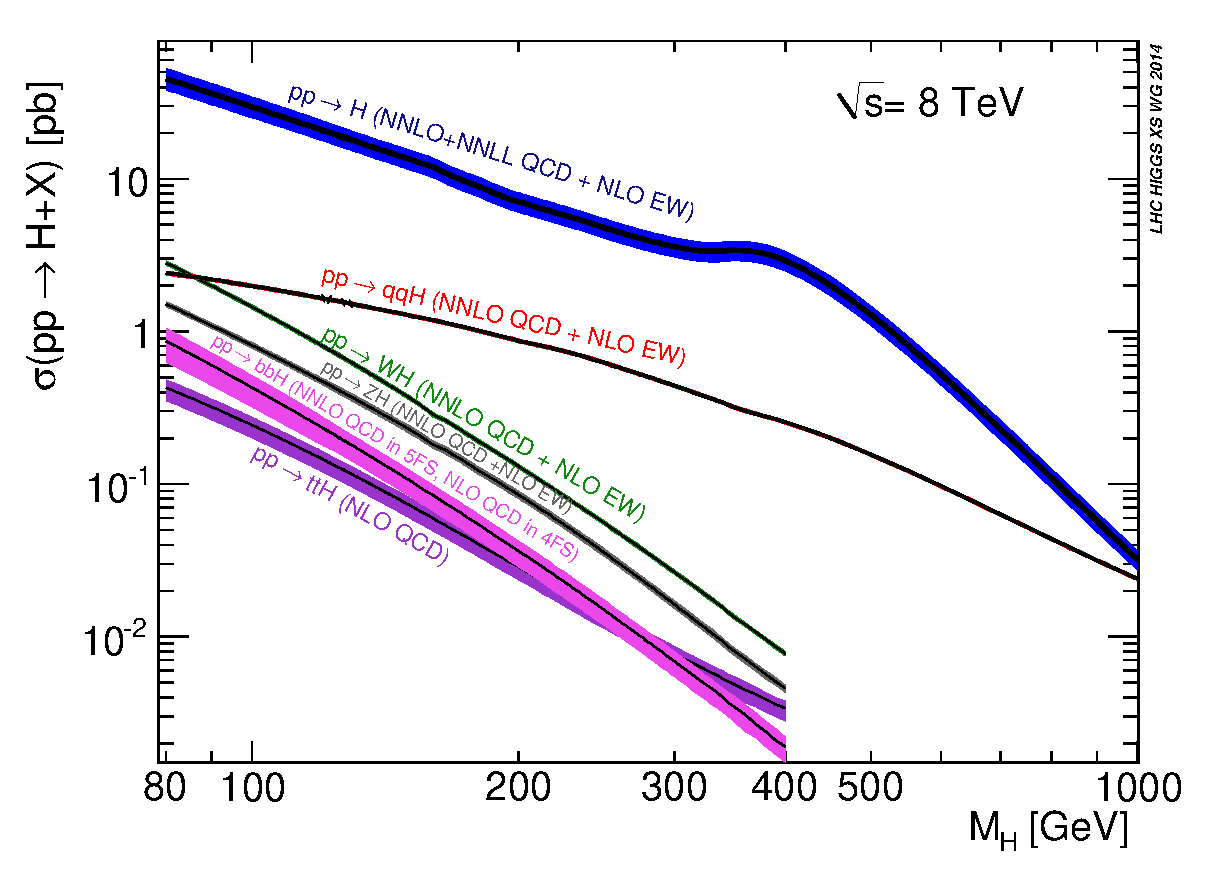
\includegraphics[width=0.56\textwidth]{\chtwo/XS_8TeV.eps}}
\subfigure[]{\label{fig:HiggsXS_b}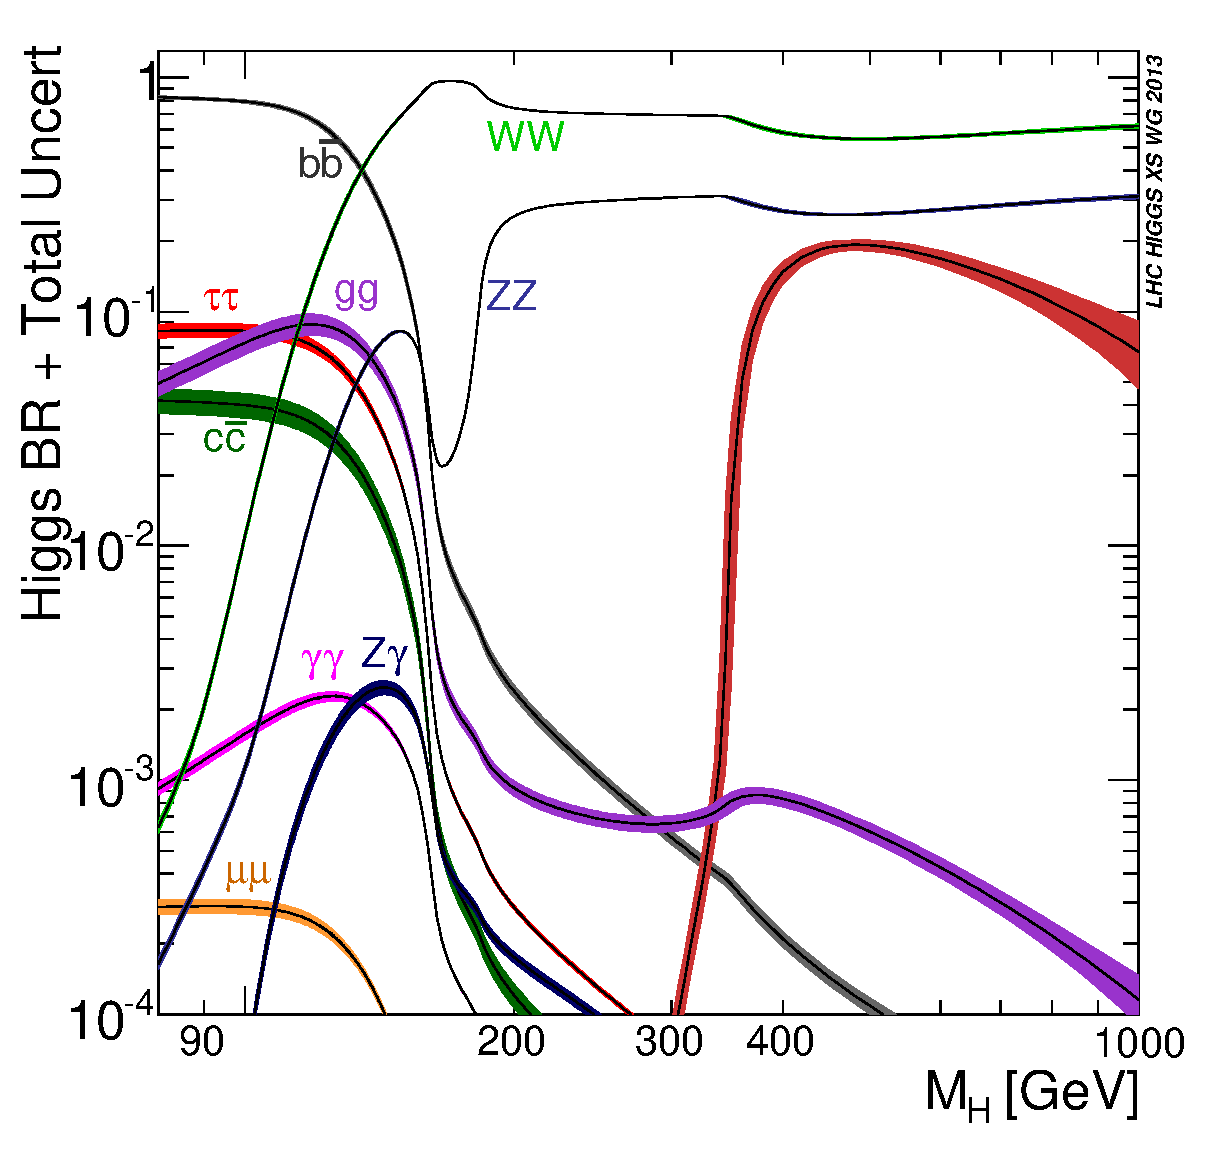
\includegraphics[width=0.42\textwidth]{\chtwo/Higgs_BR.eps}}
\caption{(a) The SM Higgs production cross-sections at $\sqrt{s} = 8\TeV$ for the different production mechanisms~\cite{Dittmaier:2011ti}. (b) Decay branching ratios of the SM Higgs boson in the different channels as a function of the mass hypothesis~\cite{Dittmaier:2011ti}.}
\label{fig:HiggsXS}
\end{figure}

\begin{figure}[!htb]
\centering
\subfigure[]{\label{fig:HiggsProd_a}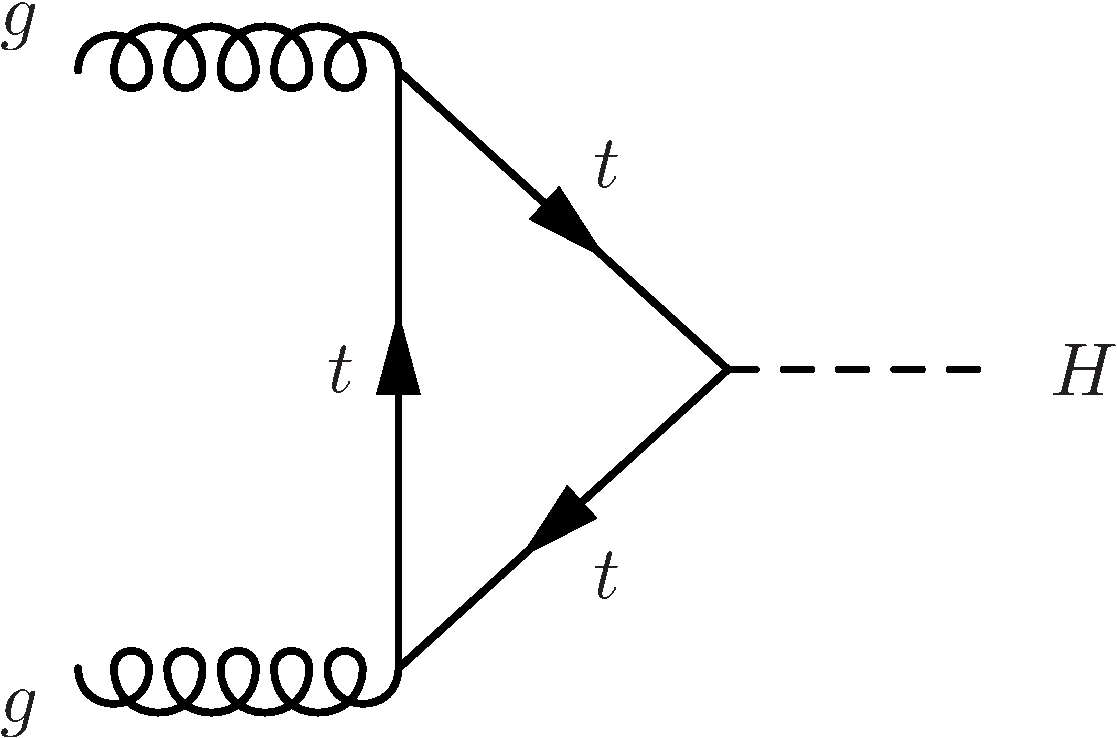
\includegraphics[width=0.23\textwidth]{\chtwo/Higgs_GF.pdf}}
\subfigure[]{\label{fig:HiggsProd_b}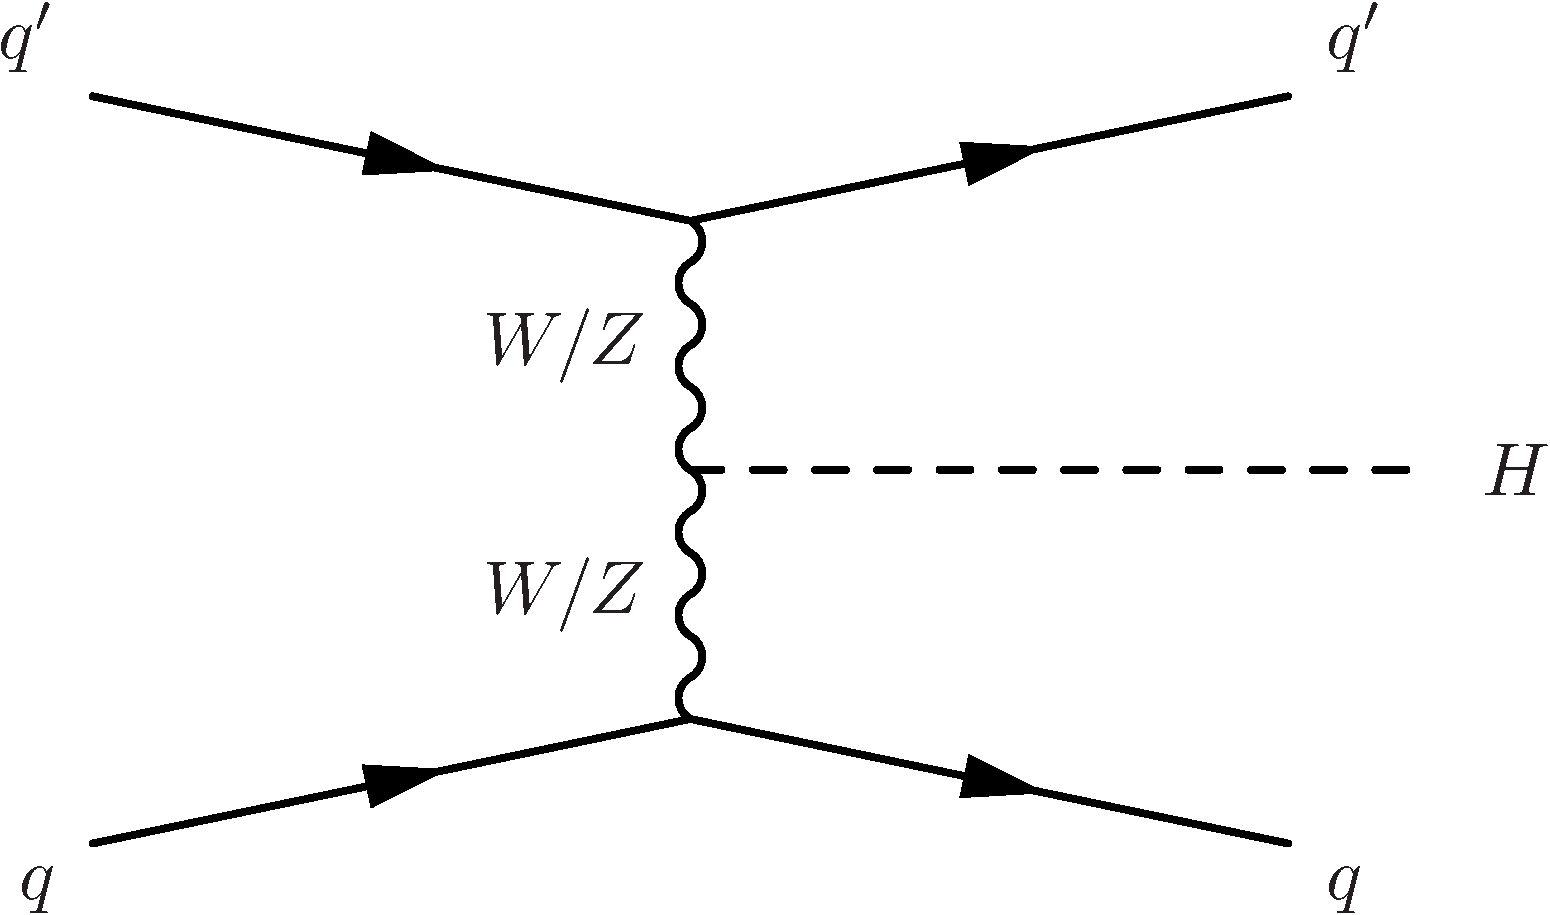
\includegraphics[width=0.23\textwidth]{\chtwo/Higgs_VBF.pdf}}
\subfigure[]{\label{fig:HiggsProd_c}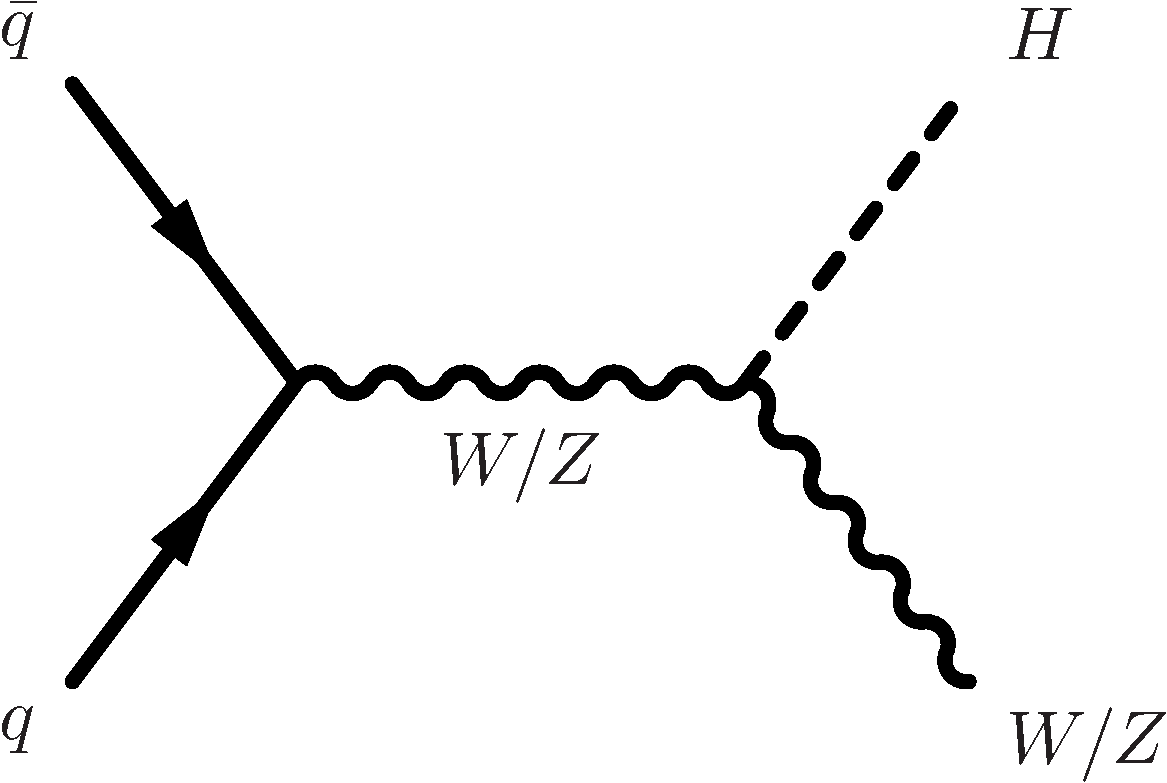
\includegraphics[width=0.23\textwidth]{\chtwo/Higgs_VH.pdf}}
\subfigure[]{\label{fig:HiggsProd_d}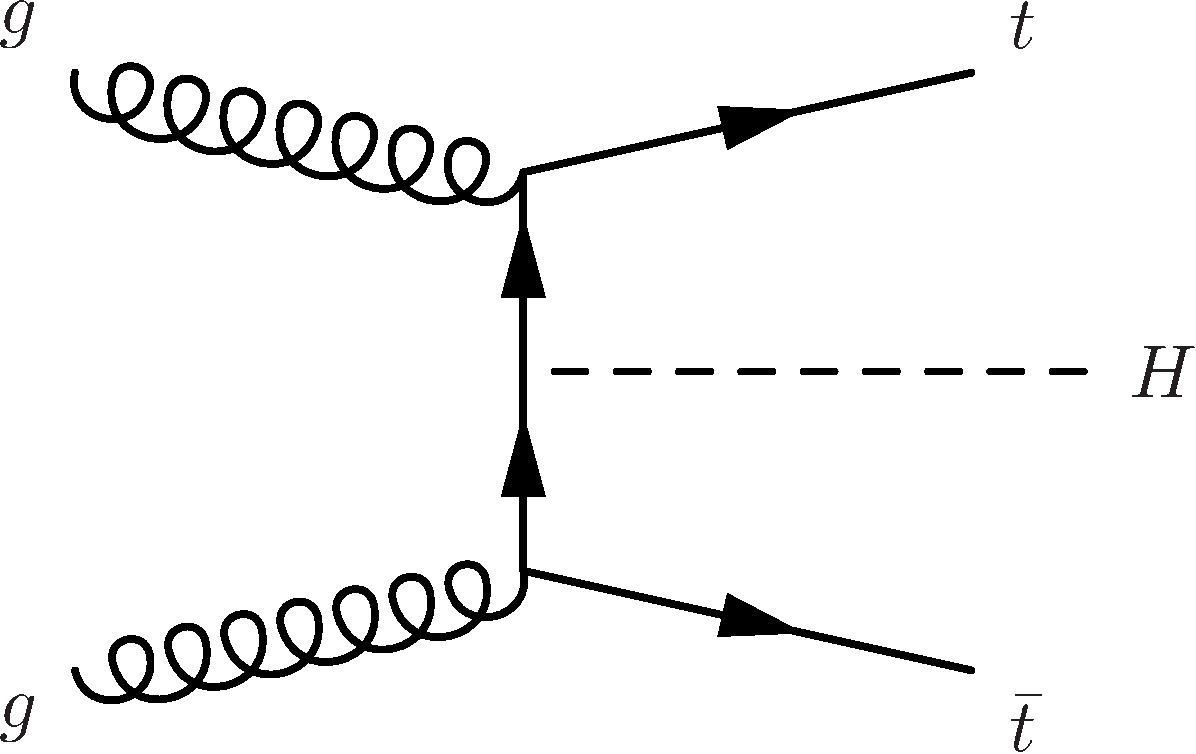
\includegraphics[width=0.23\textwidth]{\chtwo/Higgs_ttH.pdf}}
\caption{Leading order Feynman diagrams for the most important production processes of the SM Higgs boson: (a) gluon fusion, (b) vector boson fusion, (c) Higgs-strahlung and (d) \ttbar associated production.}
\label{fig:HiggsProd}
\end{figure}

The search for the massive Higgs boson has been long and tedious. 
However, in Summer 2012, the ATLAS and the CMS collaborations announced the observation of a new particle in data taken in 2011 and 2012~\cite{Chatrchyan:2013lba,Aad:2012tfa}.
A combination of the measurements targeting its decay into fermions ($\bbbar$, $\tau\tau$) or vector bosons ($\PZ\PZ^*$, $\PW\PW^*$, $\gamma\gamma$) and all the different production modes, led to an excess of events above the expected background around a mass of 125\GeV.
The CMS result yields a local significance of $5.0\sigma$ with a global significance of $4.6\sigma$ in the Higgs mass search range of $115 < m_\PH < 130\GeV$ (Fig.~\ref{fig:HiggsPvalue_a}).
For ATLAS, the local significance is found to be $5.9\sigma$ with a global significance of $5.1\sigma$ in the range $100 < m_\PH < 600\GeV$ (Fig.~\ref{fig:HiggsPvalue_b}).
A simultaneous fit to the reconstructed invariant mass peaks in the two channels with the highest mass resolution, $\PH \to \PZ\PZ^* \to 4\ell$ and $\PH \to \gamma\gamma$ , and for the two experiments has been performed.
The resulting combined measured mass of the Higgs boson is $m_\PH = 125.09 \pm 0.21 \mbox{(stat.)} \pm 0.11 \mbox{(syst.)} \GeV$ (Fig.~\ref{fig:HiggsMass})~\cite{Aad:2015zhl}.
Subsequent studies on production and decay rates~\cite{Khachatryan:2016vau} and spin-parity~\cite{Aad:2015mxa,Chatrchyan:2012jja,Khachatryan:2014kca} of the new boson showed that its properties are compatible with those expected for the SM Higgs boson. 

  \begin{figure}[!htb]
  \centering
  \subfigure[]{\label{fig:HiggsPvalue_a}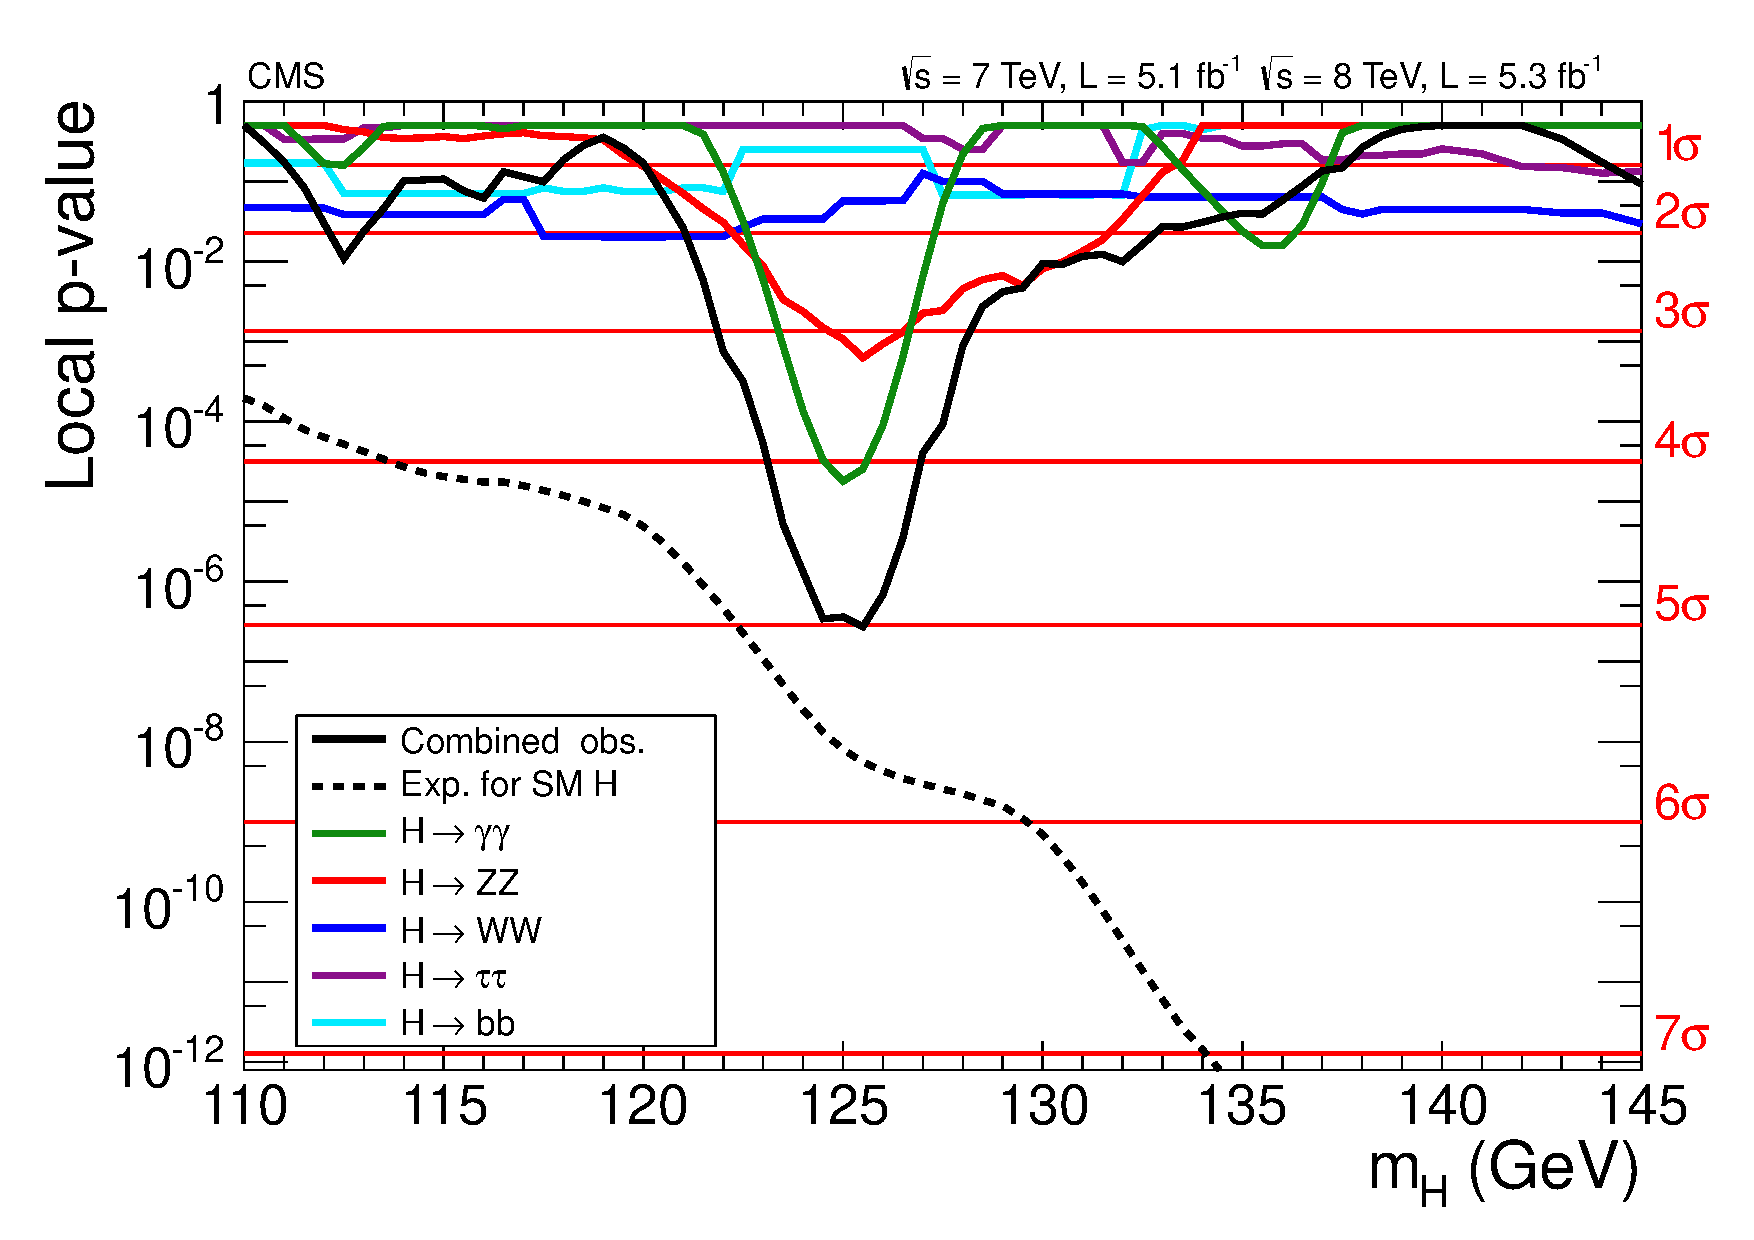
\includegraphics[width=0.45\textwidth]{\chtwo/rect_pvala_all_bydecay_smallGGScale_wideX.pdf}}
  \subfigure[]{\label{fig:HiggsPvalue_b}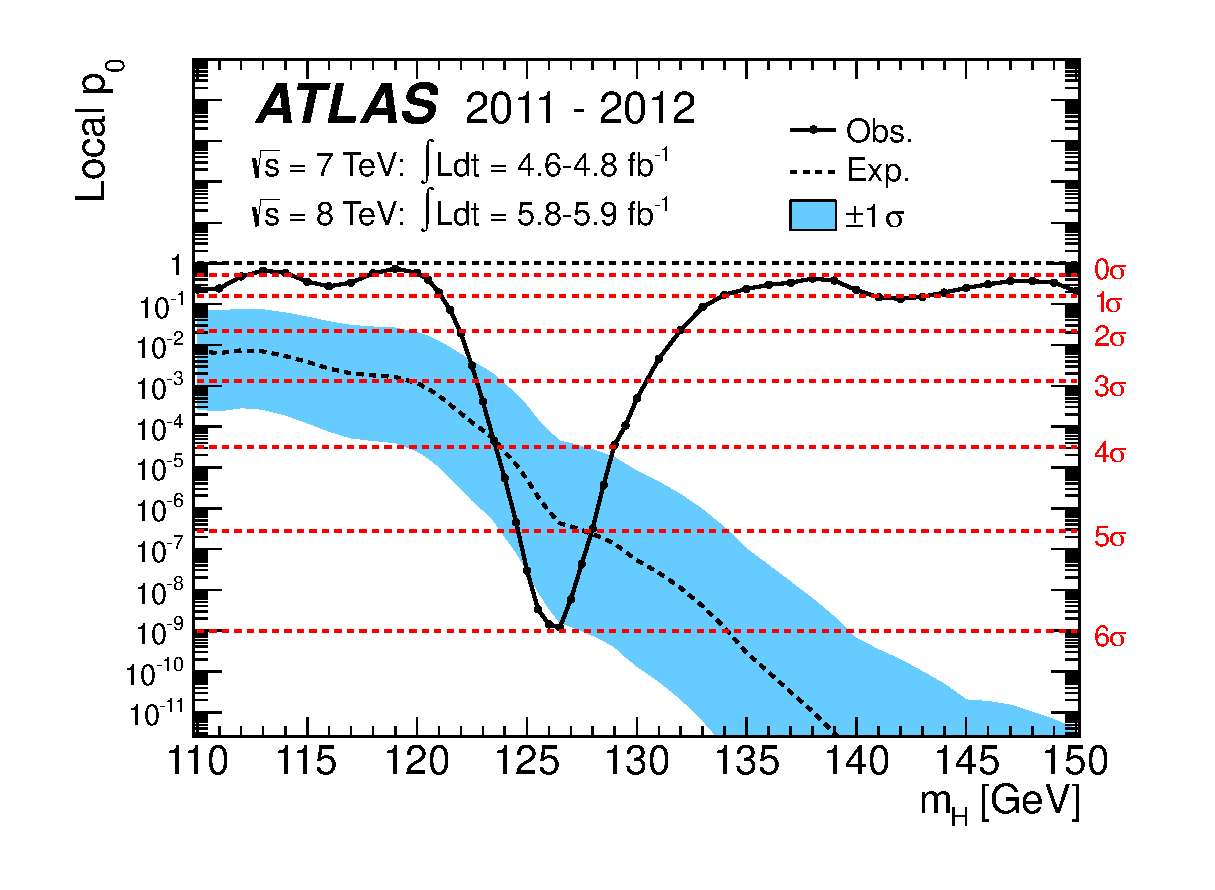
\includegraphics[width=0.45\textwidth]{\chtwo/HiggsDiscovery_ATLAS_pvalue.eps}}
  \caption{The observed (solid) local p-value as a function of the Higgs boson mass $m_\PH$ for (a) the CMS and (b) ATLAS experiments. In (a) the results for each individual channel are also shown. 
  The dashed curve shows the expected local p-value under the hypothesis of a SM Higgs boson signal at that mass.
  The horizontal red lines indicate the p-values corresponding to significances of 1 to 6$\sigma$.}
  \label{fig:HiggsPvalue}
\end{figure} 

  \begin{figure}[!htb]
  \centering
  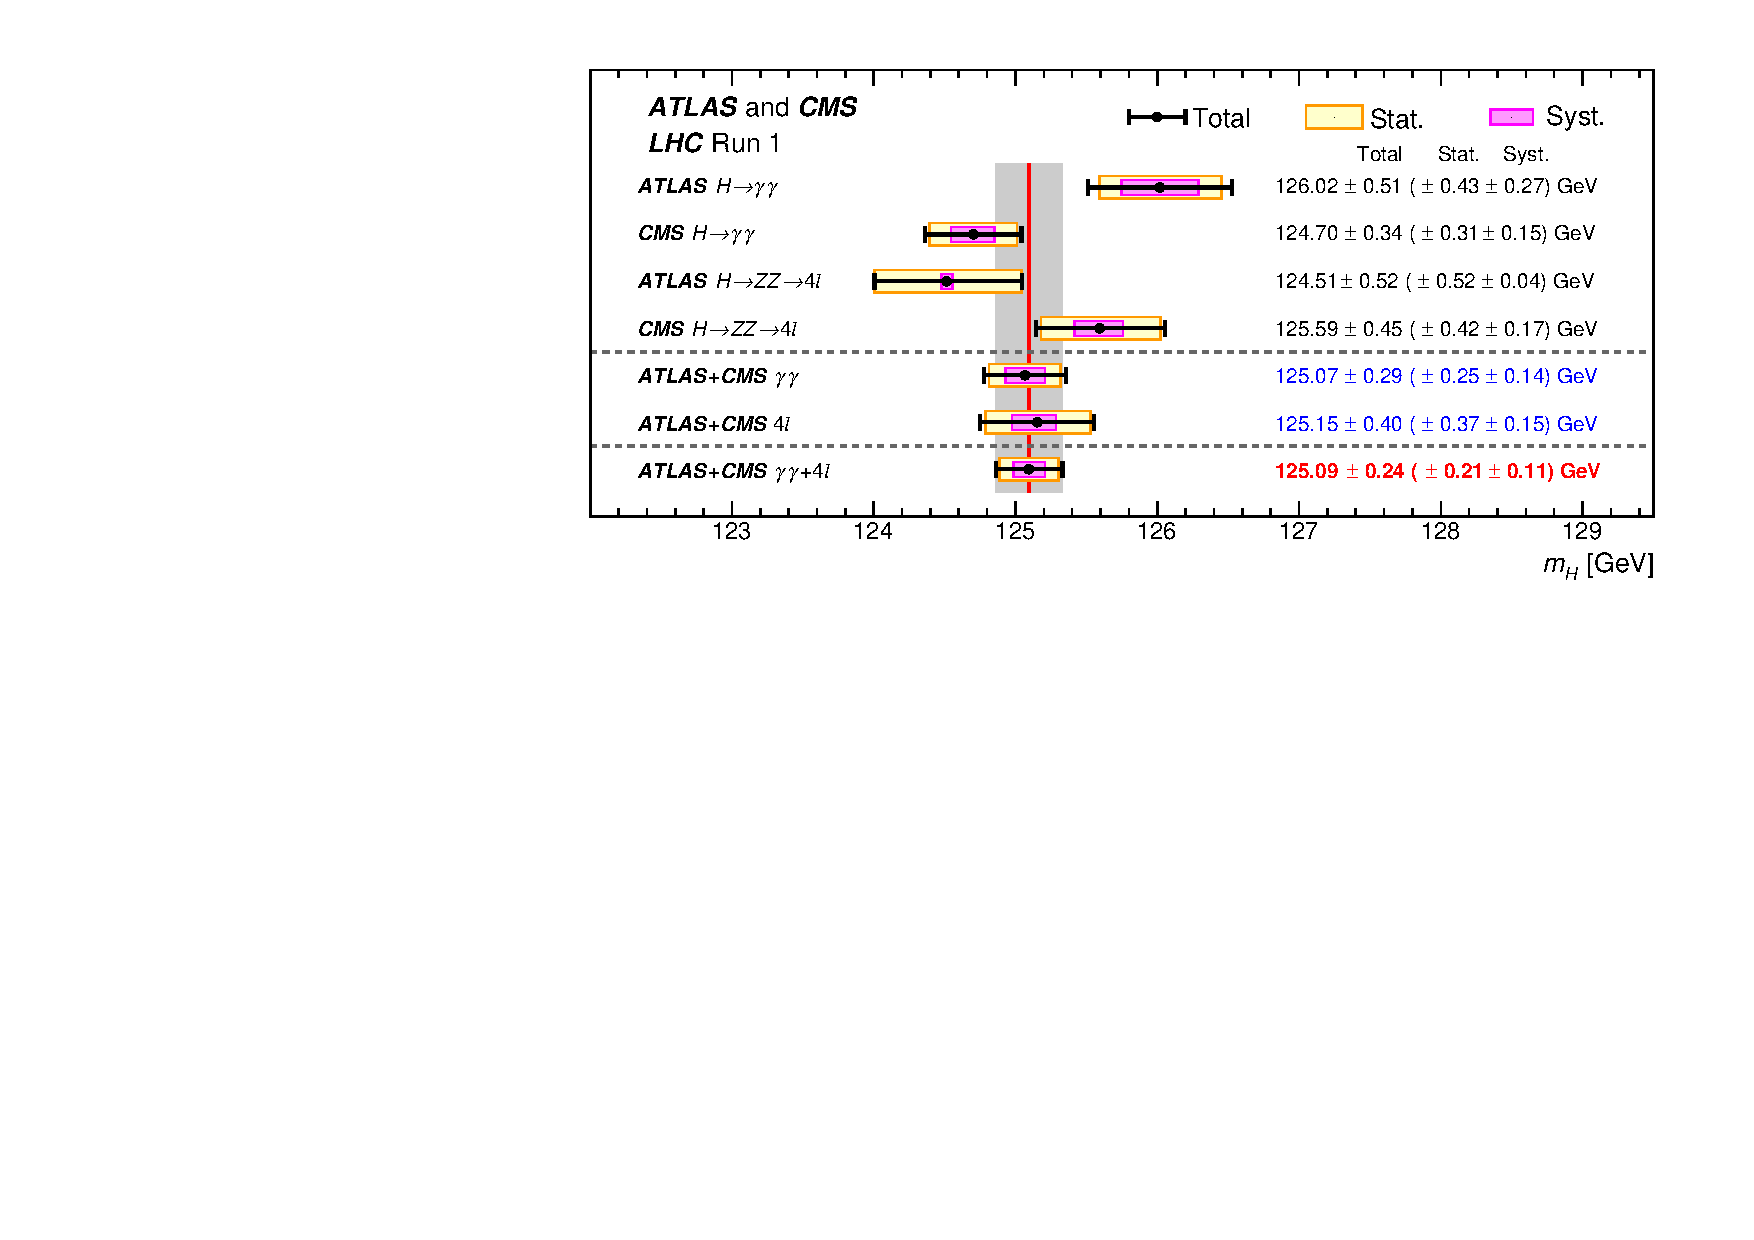
\includegraphics[width=0.7\textwidth]{\chtwo/LHC_combined_obs_unblind_summary_a1_final.pdf}
  \caption{Summary of Higgs boson mass measurements from the individual analyses of ATLAS and CMS and from their combination.
  The magenta and yellow bands correspond to the the systematic and statistical uncertainties, respectively. The total uncertainties are also indicated as black error bars.
  The red vertical line and corresponding gray shaded column indicate the central value and the total uncertainty of the combined measurement, respectively~\cite{Aad:2015zhl}.}
  \label{fig:HiggsMass}
\end{figure} 

Finally, the Higgs boson couplings to SM particles are investigated simultaneously in different production and decay processes, including the possibility of the Higgs boson to be coupled to BSM particles~\cite{Khachatryan:2016vau}.
To test possible deviations from the SM predictions, the coupling modifiers, $k^2_j = \sigma_j/\sigma^\mathrm{SM}_j$ and $k^2_j = \Gamma_j/\Gamma^\mathrm{SM}_j$, for production and decay rates, are introduced. 
However, to directly measure the individual coupling modifiers, an assumption about the Higgs boson width $\Gamma_\PH$ is necessary. Thus, another modifier is introduced and defined as $k_\PH = \sum_j \mathcal{B}^\mathrm{SM}_jk^2_j$, where $\mathcal{B}^\mathrm{SM}_j$ are the branching fractions for the Higgs boson decay to the final state $f$ as predicted by the SM. In the case where the SM decays of the Higgs boson are the only ones allowed,
the relation $k^2_\PH = \Gamma_\PH/\Gamma^\mathrm{SM}_\PH$ holds. If instead deviations from the SM are introduced in the decays, the width can be expressed as:

\begin{equation}\label{eqn:SM_e45}
\Gamma_\PH = \frac{k^2_\PH\Gamma^\mathrm{SM}_\PH}{1 - B_\mathrm{BSM}},
\end{equation}

\noindent where $B_\mathrm{BSM}$ indicates the total branching fraction into BSM decays.
The two possible scenarios are considered: the first leaves $B_\mathrm{BSM}$ free, provided that $B_\mathrm{BSM} \geq 0$, whereas the second assumes $B_\mathrm{BSM} = 0$. 
The parameters of interest in the fits to data are thus the seven independent coupling modifiers, $k_\PZ$, $k_\PW$, $k_\mathrm{t}$, $k_\tau$, $k_\mathrm{b}$, $k_g$, and $k_\gamma$, 
one for each SM particle involved in the production processes and decay modes studied, plus $B_\mathrm{BSM}$ in the case of the first scenario.
The results of the two fits are shown in Fig.~\ref{fig:HiggsCoupl}.
The overall branching fraction of the Higgs boson into BSM decays is determined to be less than 34\% at 95\% CL.
This constraint applies to invisible decays into BSM particles, decays into BSM particles that are not detected as such, and modifications of the decays into SM particles that are not directly measured by the experiments.

  \begin{figure}[!htb]
  \centering
  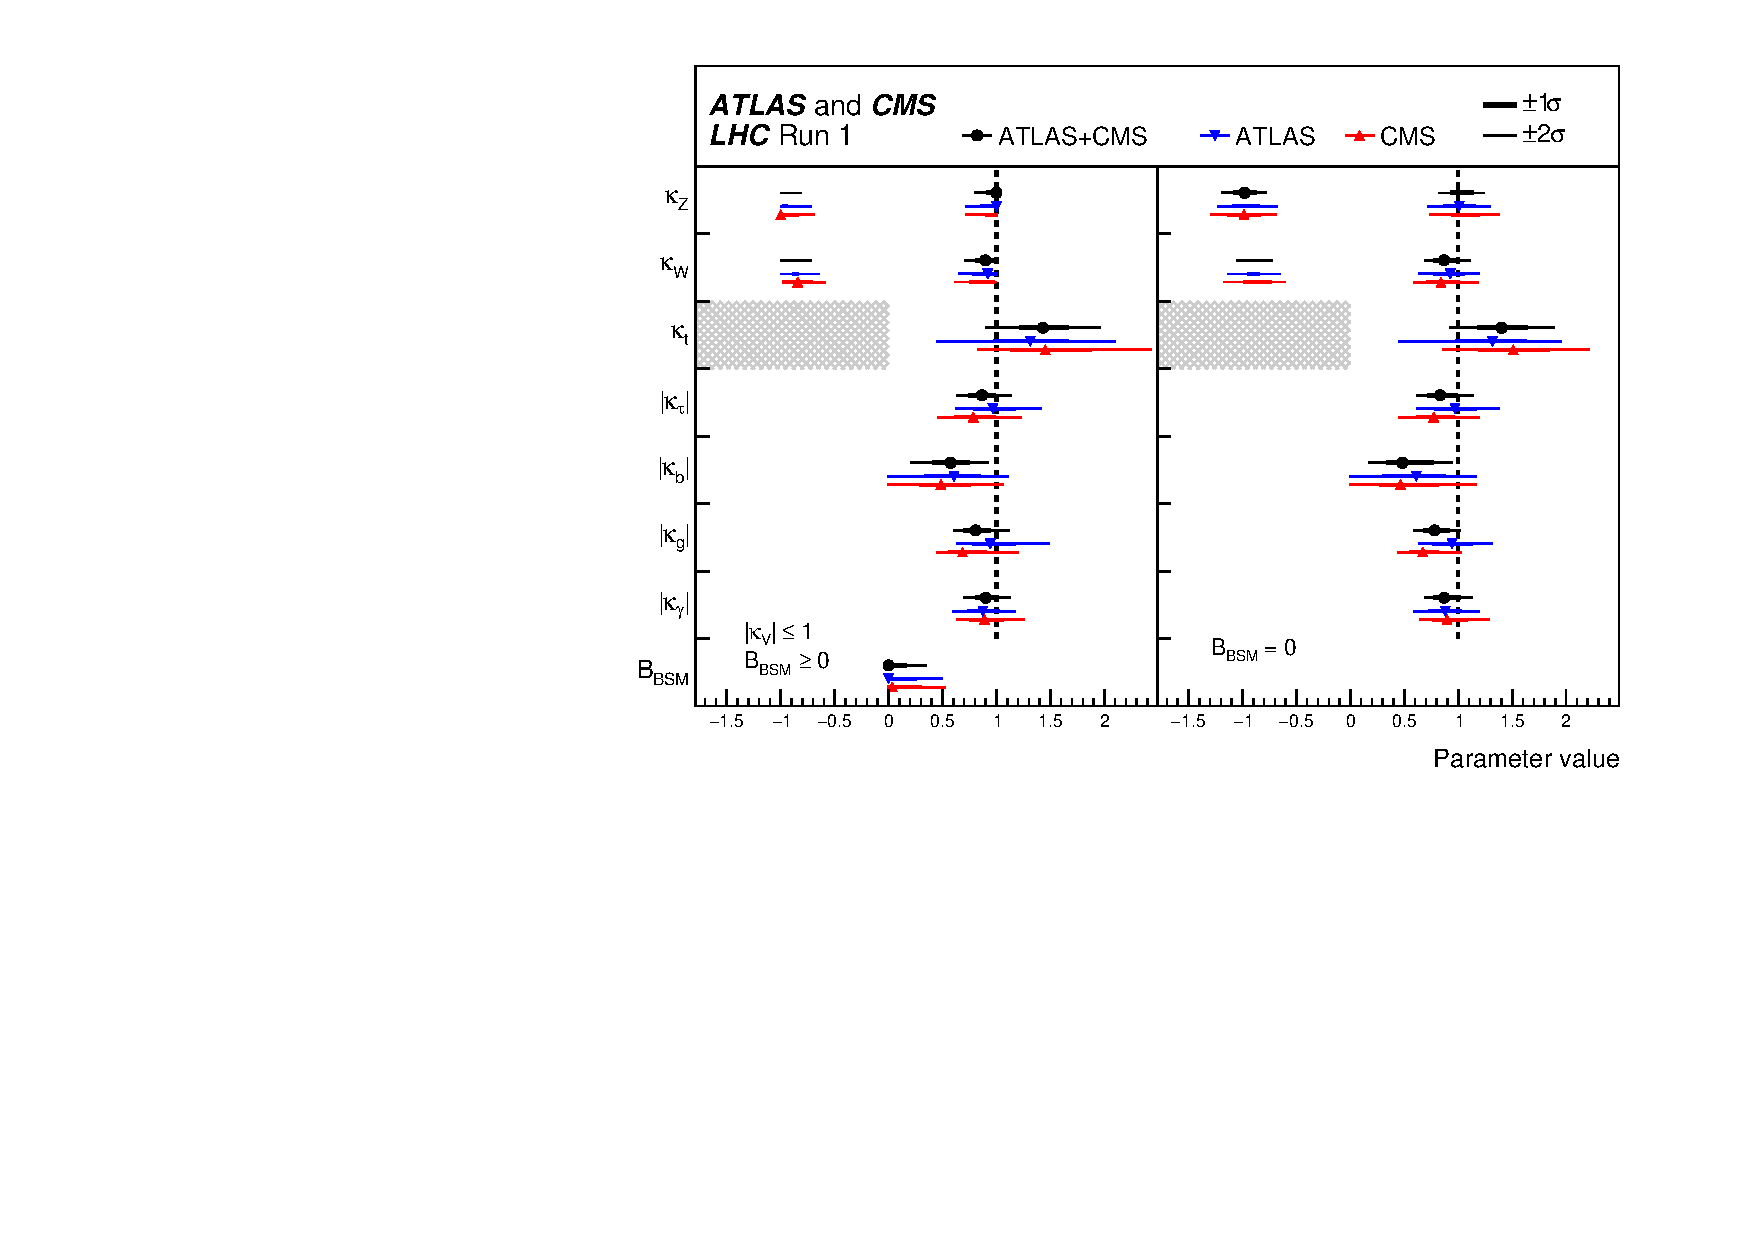
\includegraphics[width=0.7\textwidth]{\chtwo/plot_K2_K2_BRinv_per_exp_merged.pdf}
  \caption{Fit results for two parameterizations: the first one assumes that $B_\mathrm{BSM} \geq 0$, and the second one assumes that there are no additional BSM contributions to the Higgs boson width ($B_\mathrm{BSM} = 0$). The measured results for the combination of ATLAS and CMS are reported together with their uncertainties, as well as the individual results from each experiment~\cite{Aad:2015zhl}.}
  \label{fig:HiggsCoupl}
\end{figure} 

%%%%%%%%%%%%%%%%%%%%%%%%%%%%%%%%%%%%%%%%%
\subsection{Quantum chromodynamics}\label{subsec:QCD}
%%%%%%%%%%%%%%%%%%%%%%%%%%%%%%%%%%%%%%%%%

Quantum Chromodynamics (QCD) is the gauge theory of strong interactions, describing the dynamics of colored quarks and gluons.
The QCD represents the $SU(3)_C$ component of the standard model, where $C$ denotes the color.
After applying the principle of gauge invariance to the free Lagrangian for the quark fields holding color $\alpha$ that runs from 1 to 3 (usually identified with red, green, blue), and flavor $q$, one obtains the following expression for the final gauge invariant QCD Lagrangian

\begin{equation}\label{eqn:SM_e46}
\mathcal{L}_\mathrm{QCD} = \sum_{q} \bar{\psi}_{q,\alpha} (i\gamma^\mu\partial_\mu\delta_{\alpha\beta} - g_s\gamma^\mu t^a_{\alpha\beta}\mathcal{A}^a_\mu - m_q\delta_{\alpha\beta})\psi_{q,b} - \frac{1}{4}G^a_{\mu\nu}G^{\mu\nu}_a.
\end{equation}

In the equation above, the quark fields are represented by the spinors $\psi$. The fields $\mathcal{A}^a_\mu$ corresponds to the eight gluon fields, since $C$ runs from 1 to $N^2_C - 1 = 8$.
Each gluon carries one unit of color and one unit of anticolor.
The eight $3\times3$ matrices $t^a_{\alpha\beta}$ are the $SU(3)_C$ generators and rotate the quark color in the $SU(3)_C$ space in a quark-gluon interaction.
The field tensor is

\begin{equation}\label{eqn:SM_e47}
G^a_{\mu\nu} = \partial_\mu\mathcal{A}^a_\nu - \partial_\nu\mathcal{A}^a_\mu - g_s f_{abc}\mathcal{A}^b_\mu\mathcal{A}^c_\nu,
\end{equation}

\noindent where $f_{abc}$ are the structure constants of the $SU(3)$ group.
As $[t^a,t^b] = if_{abc}t^c$ the group is non-Abelian. Owing this property, $G^a_{\mu\nu}G^{\mu\nu}_a$ term generates the cubic and quartic gluon self-interactions.
The fundamental parameters of QCD are the \textit{strong coupling constant} $g_s$, often written in terms of $\alpha_s = g_s^2/4\pi$, and the quark masses $m_q$.
All interactions appearing in Eq.~\ref{eqn:SM_e45} have strength given by $g_s$ (Fig.~\ref{fig:QCDVtx}).\\

\begin{figure}[!htb]
\centering
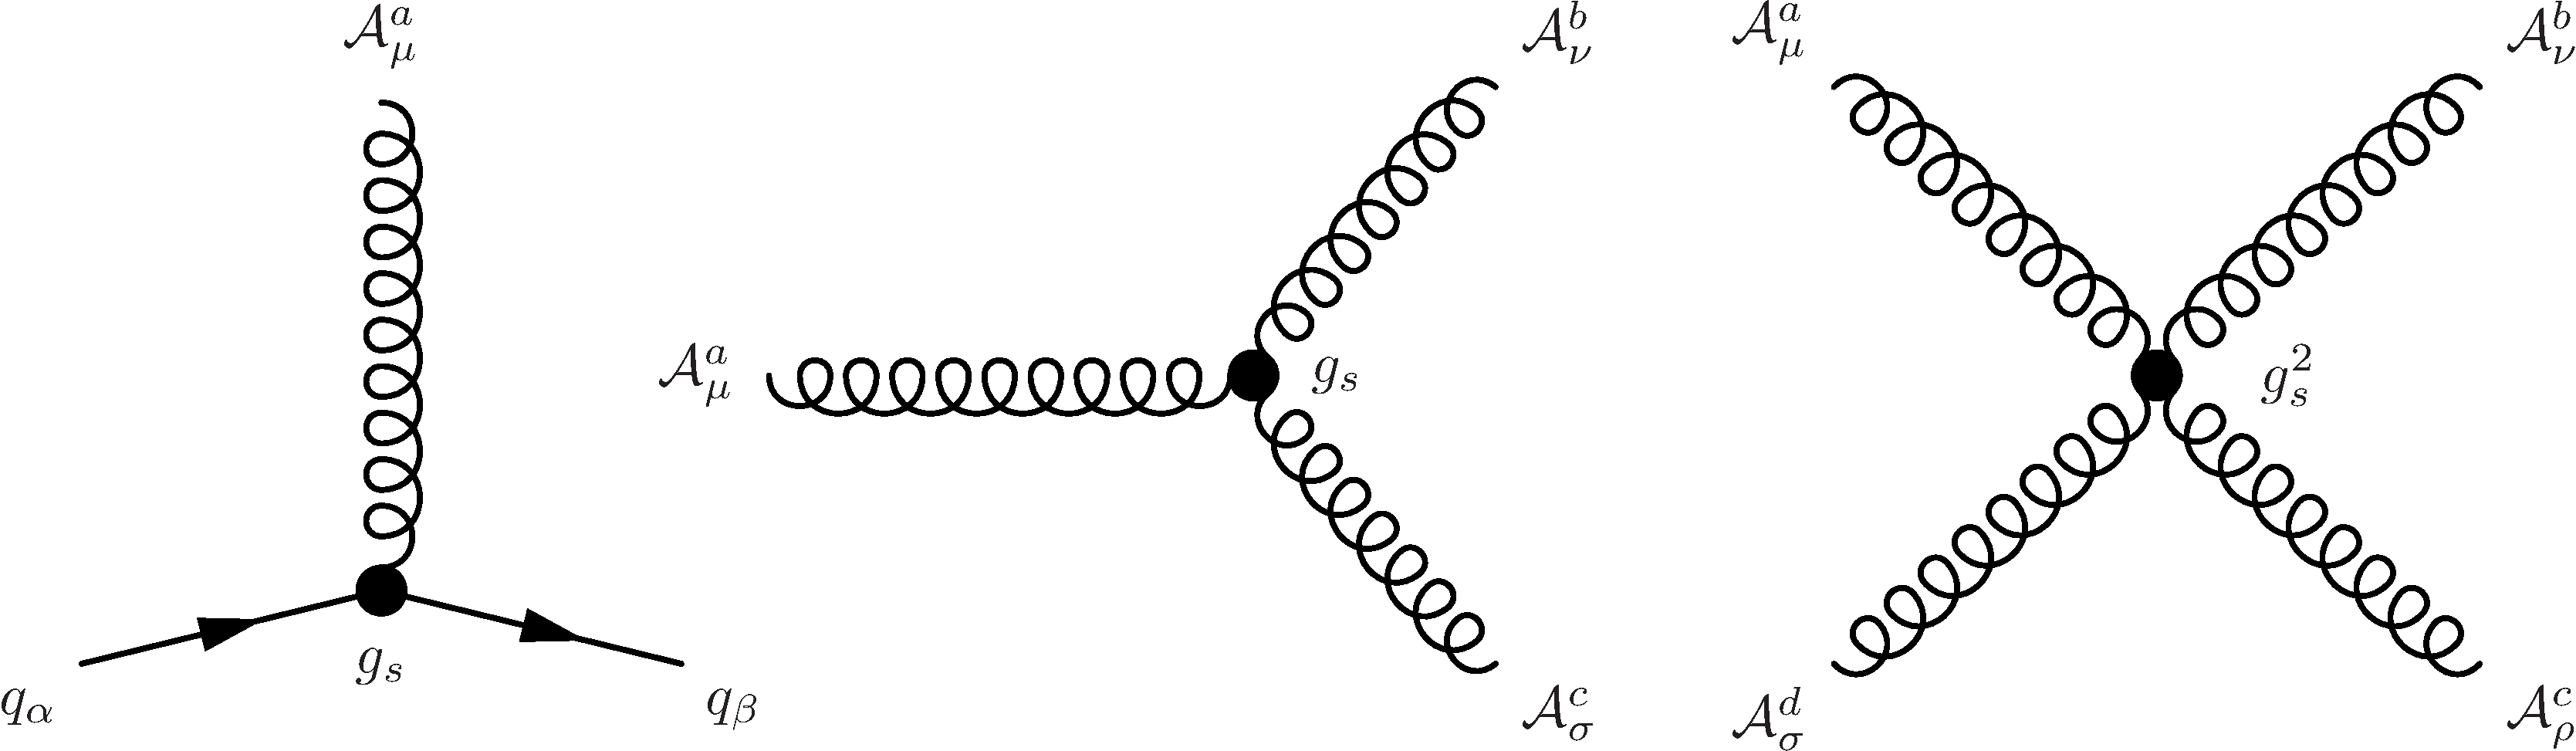
\includegraphics[width=0.9\textwidth]{\chtwo/QCD_vtx.pdf}
\caption{Interaction vertices of the QCD Lagrangian.}
\label{fig:QCDVtx}
\end{figure}

The QCD has the property of \textit{asymptotic freedom}, i.e. the coupling becomes weak at high energies or short distances, and for energies approaching zero or for very large distances, it tends to infinity.
As a consequence, the further away a quark is pulled from another one, the stronger the force gets, such that quarks cannot exist as free particles.
Because of this phenomenon, referred to as \textit{confinement}, quarks form bound color-singlet states called hadrons, consisting of either a quark and an antiquark (mesons) or three quarks or antiquarks (baryons).
%As a consequence, only in very high momentum transfer interactions, quarks can be regarded as free particles, whereas at low energy or large distance, the interaction becomes strongly coupled leading to \textit{confinement} of quarks %and gluons. Instead, they form bound color-singlet states called hadrons, consisting of either a quark and an antiquark (mesons) or three quarks or antiquarks (baryons).
%In this process, after a quark production, at very short distances, the quantum nature of QCD predicts the generation of virtual quark-antiquark (or gluons) pairs, which couple together through color strings forming observable un-%colored baryons and mesons.
In the regime of very high momentum transfer interactions, the perturbation theory is a very satisfactory description of QCD physics observables, giving precise predictions about what can be tested in collider experiments. This approach is called perturbative-QCD, or pQCD. In this framework, QCD predictions are calculated using the formalism of the Feynman rules which are derived from the $\mathcal{L}_\mathrm{QCD}$.
The transition amplitudes for a given process from a set of initial state particles to a set of final state particles are computed by sorting the diagrams by the factors of the coupling constants and calculating them up to a certain order.
However, higher order diagrams generally contain loops which contribute and lead to divergencies.
In order to obtain finite predictions for the cross sections, a renormalization of the theory is performed, resulting in a cancellation of the divergent terms.
%The divergencies are absorbed into a redefinition of the color charge. As a consequence of this, $\alpha_s$ is a running coupling constant as a function of a renormalization scale $\mu_R$, and is given by
The predictions for observables are then expressed in terms of the renormalized coupling $\alpha_s(\mu^2_R)$, a function of the renormalisation scale $\mu_R$. 
The coupling satisfies the renormalisation group equation:

\begin{equation}\label{eqn:SM_e48}
\mu^2_R\frac{\mathrm{d}\alpha_s}{\mathrm{d}\mu^2_R} = \beta(\alpha_s) = - (b_0\alpha^2_s + b_1\alpha^3_s + b_2\alpha^4_s + \dotsc)
\end{equation}

\noindent where the $b_i$ are the $i$-loop coefficients of the $\beta$ function.
They depend on the number of quark flavors $n_f$, and for sixteen or less flavors the strong coupling gets smaller for processes that involve large momentum transfer, leading to the asymptotic freedom.
Choosing $\mu_R$ close to the typical scale of the process of interest $Q^2$, the $\alpha_s(\mu_R)$ represents the effective strength of the strong interaction between particles under study.
Neglecting all the $b_i$ coefficients but $b_0$, an exact leading order expression for the running coupling $\alpha_s$ can be obtained

\begin{equation}\label{eqn:SM_e49}
\alpha_s(\mu^2_R) = \frac{1}{b_0\log \left( \frac{\mu^2_R}{\Lambda^2_\mathrm{QCD}} \right) } = \frac{12\pi}{(33-2n_f)\log \left( \frac{\mu^2_R}{\Lambda^2_\mathrm{QCD}} \right) }
\end{equation}

\noindent where $\Lambda_\mathrm{QCD}$ is the perturbative cut-off over the renormalization's integrals, and is not predicted by the theory.
The meaning of this cut-off is the validity of the perturbative regime approximation, beyond which the integrals would diverge.
For many experimental studies, the strong coupling is evaluated at a fixed energy scale, typically of the order of the electroweak scale, $\mu_R \simeq M_\PZ$ (Fig.~\ref{fig:AlphaS}).

\begin{figure}[!htb]
  \centering
  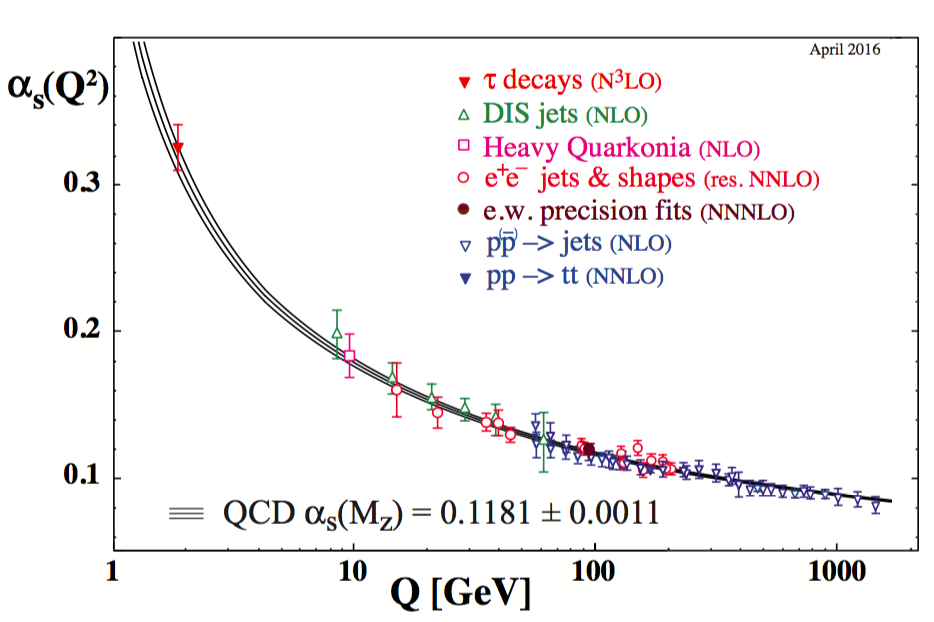
\includegraphics[width=0.6\textwidth]{\chtwo/alphaS_measurement_2016.png}
  \caption{Summary of measurements of the running coupling $\alpha_s$ as a function of the energy scale $Q$ of the process~\cite{Olive:2016xmw}.}
  \label{fig:AlphaS}
\end{figure} 

%\section{Theories of new physics}
  %%%%%%%%%%
\section{Limitations of the standard model}
\label{sec:SMLimitations}
%%%%%%%%%%

The standard model has been remarkably confirmed by experimental data collected over the last few decades, validating most of its predictions.
The ultimate verification of the model has been provided by the latest discovery of a scalar particle at the LHC (Section~\ref{subsec:HiggsLHC}), whose properties are statistically compatible with the SM predictions for the Higgs boson.
Nevertheless, there are fundamental physical phenomena in nature that cannot be adequately explained by the SM. %as well as theoretical deficiencies that make the model unsatisfactory.
Furthermore, some features of the model represent \textit{ad hoc} additions to the theory and, although providing predictions that have been confirmed, imply a lack of understanding, making the framework theoretically unsatisfactory.
Some of the main unresolved issues of the SM are briefly described in the following.

\subsection*{The hierarchy problem}

This issue arises from the observation of a large discrepancy between the electroweak and gravitational scales. This is reflected in the mass difference between the masses of the \PW and \PZ bosons that define the scale of electroweak interactions ($\mathcal{O}(10^2\GeV)$), and the Planck mass ($\MPl = \sqrt{\hbar c/G_\mathrm{Newton}} = \mathcal{O}(10^{19})$), that defines the scale beyond which the gravitational force must be described by quantum mechanics. This feature is commonly known as \textit{hierarchy problem} or as well problem of \textit{naturalness}, meaning an ``unnatural'' or equivalently ``unexpected'' behaviour.
More technically, the question is why the measured Higgs-boson mass $(M_\PH)_{measured} \approx 125\GeV$ is so much smaller than the Planck mass.
%\begin{wrapfigure}{R}{0.4\textwidth}
 %\centering
 %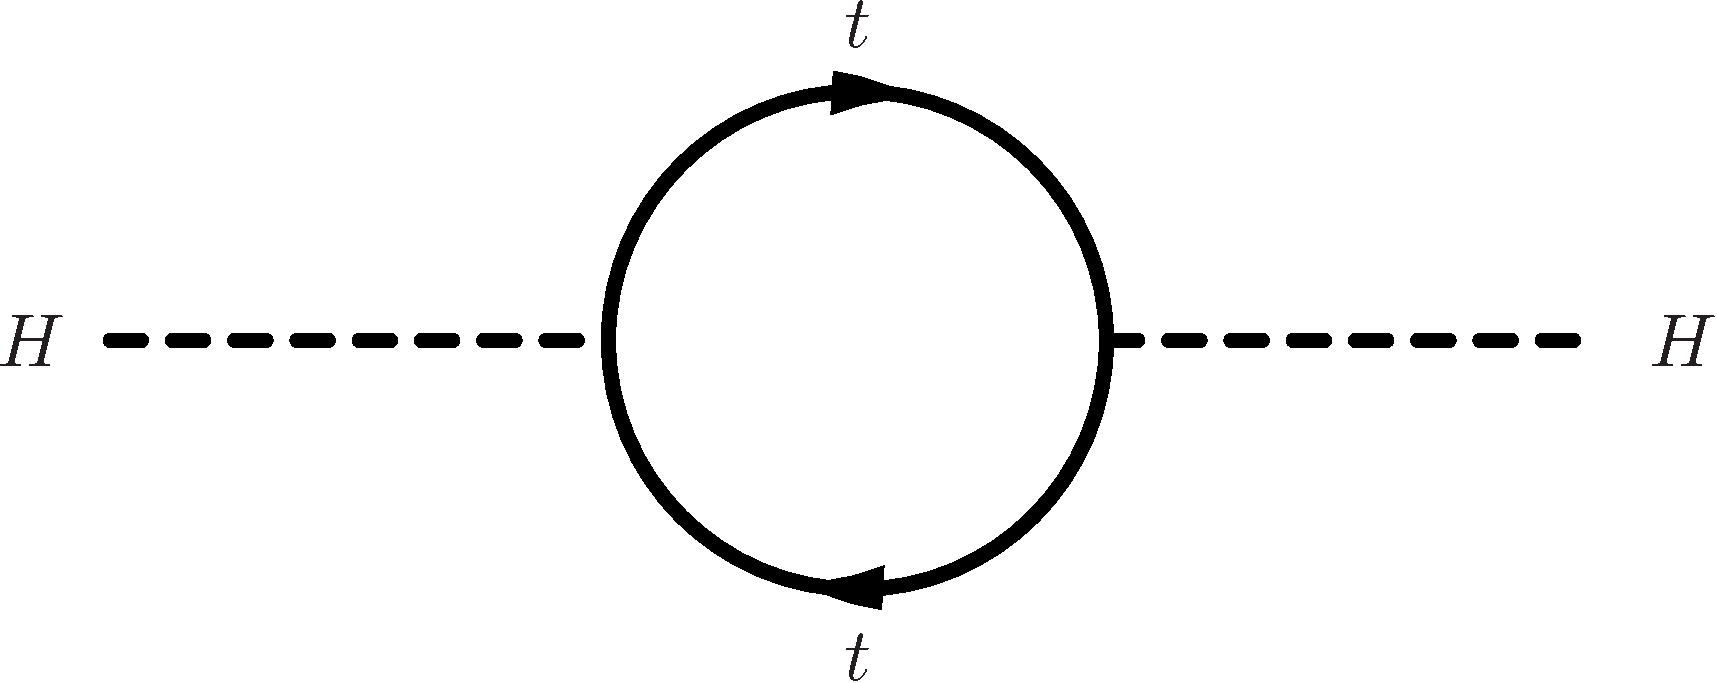
\includegraphics[width=0.35\textwidth]{\chtwo/HiggsLoop.pdf}
 %\caption{One-loop quantum corrections to the Higgs squared mass parameter $m^2_\PH$ due to a fermion $f$.}
 %\label{fig:HiggsLoop}
%\end{wrapfigure}
The problem is that the tree-level Higgs-boson mass $M^2_\PH$ (Eq.~\ref{eqn:SM_e38}) receives quadratically-divergent corrections from the virtual effects of every particle that couples, directly or indirectly, to the Higgs field.
%For example, the Feynman diagram in Fig.~\ref{fig:HiggsLoop} brings a correction to $m^2_\PH$ from a loop containing a fermion $f$ with mass $m_f$.
%If the Higgs field $H$ couples to $f$ with a term in the Lagrangian $-\lambda_fH\bar{f}f$, where $\lambda_f$ is the Yukawa coupling, then this loop yields a correction
%\begin{equation}\label{eqn:HiggsCorr}
%\delta m^2_\PH = - \frac{|\lambda_f|^2}{8\pi^2}\Lambda^2 + \dotsc,
%\end{equation}
%\noindent where $\Lambda$ is a momentum cut-off representing the scale up to which the SM remains valid, and beyond which new physics enters to alter the high-energy behavior of the theory.
There are three types of corrections to the Higgs-boson mass that arise from the diagrams in Fig.~\ref{fig:HiggsLoop}.
Each of them gives a correction to the Higgs-boson mass:

\begin{equation}\label{eqn:HiggsCorr}
\begin{aligned}
\mbox{top loop} & \qquad\qquad\qquad\qquad -\frac{3}{8\pi^2}\lambda_t\Lambda^2\\
\mbox{gauge loop} & \qquad\qquad\qquad\qquad + \frac{1}{16\pi^2}g^2\Lambda^2\\
\mbox{Higgs loop} & \qquad\qquad\qquad\qquad + \frac{1}{16\pi^2}\lambda^2\Lambda^2\\
\end{aligned}
\end{equation}

\noindent where $\lambda_t$ is the Yukawa coupling with the top quark, $g$ is the gauge coupling, $\lambda$ is the Higgs self coupling, and $\Lambda$ represents the energy scale up to which the SM remains valid, and beyond which an unknown new physics theory enters to alter the high-energy behavior of the theory.
Each of the leptons and quarks of the SM also contribute, however the largest correction arises from the top quark.
%Each of the leptons and quarks of the SM can play the role of $f$ and the largest correction arises when $f$ is the top quark.
If $\Lambda$ is of the order of \MPl, then this correction to $M^2_\PH$ is about 30 orders of magnitude larger than the measured value of 125\GeV.
Thus, in order to obtain such a small value for the Higgs-boson mass an incredible fine-tuning cancellation must occur between the tree-level value and the correction.
Avoiding such a miraculous cancellation can only happen if the cut-off scale is $\Lambda \simeq \mathcal{O}(1 - 10\TeV)$ rather than the Planck scale, which implies that new physical processes show up at that energy.
This is only directly a problem for corrections to the Higgs scalar boson squared mass, because quantum corrections to fermion and gauge boson masses do not have the direct
quadratic sensitivity to $\Lambda$ found in Eq.~\ref{eqn:HiggsCorr}. However, the quarks and leptons and the electroweak gauge bosons of the SM all obtain masses from the Higgs boson,
so that the entire mass spectrum of the theory is directly or indirectly sensitive to the cut-off $\Lambda$.

\begin{figure}[!htb]
 \centering
 \subfigure[]{\label{fig:HiggsLoop_a}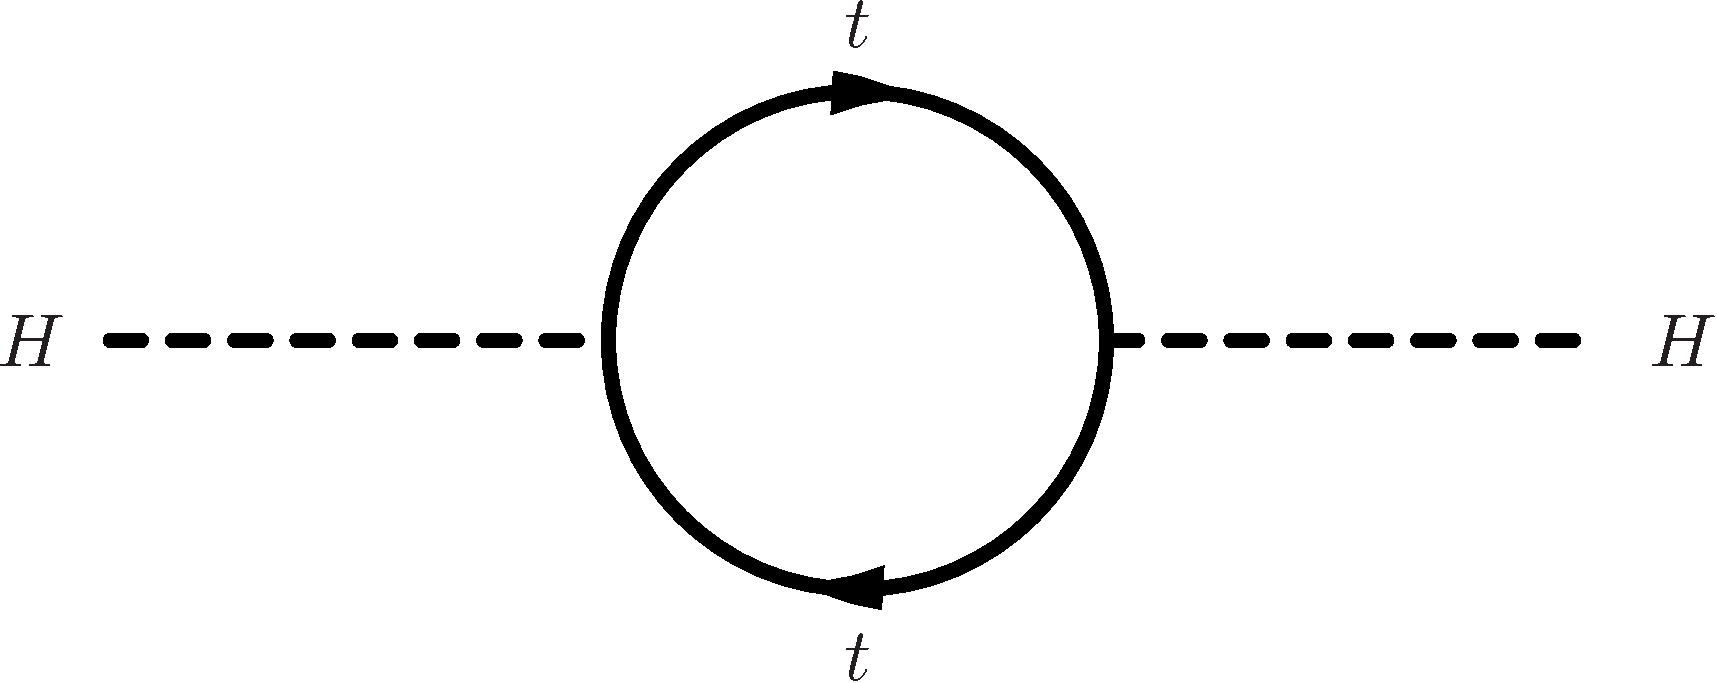
\includegraphics[width=0.3\textwidth]{\chtwo/HiggsLoop.pdf}}
 \subfigure[]{\label{fig:HiggsLoop_b}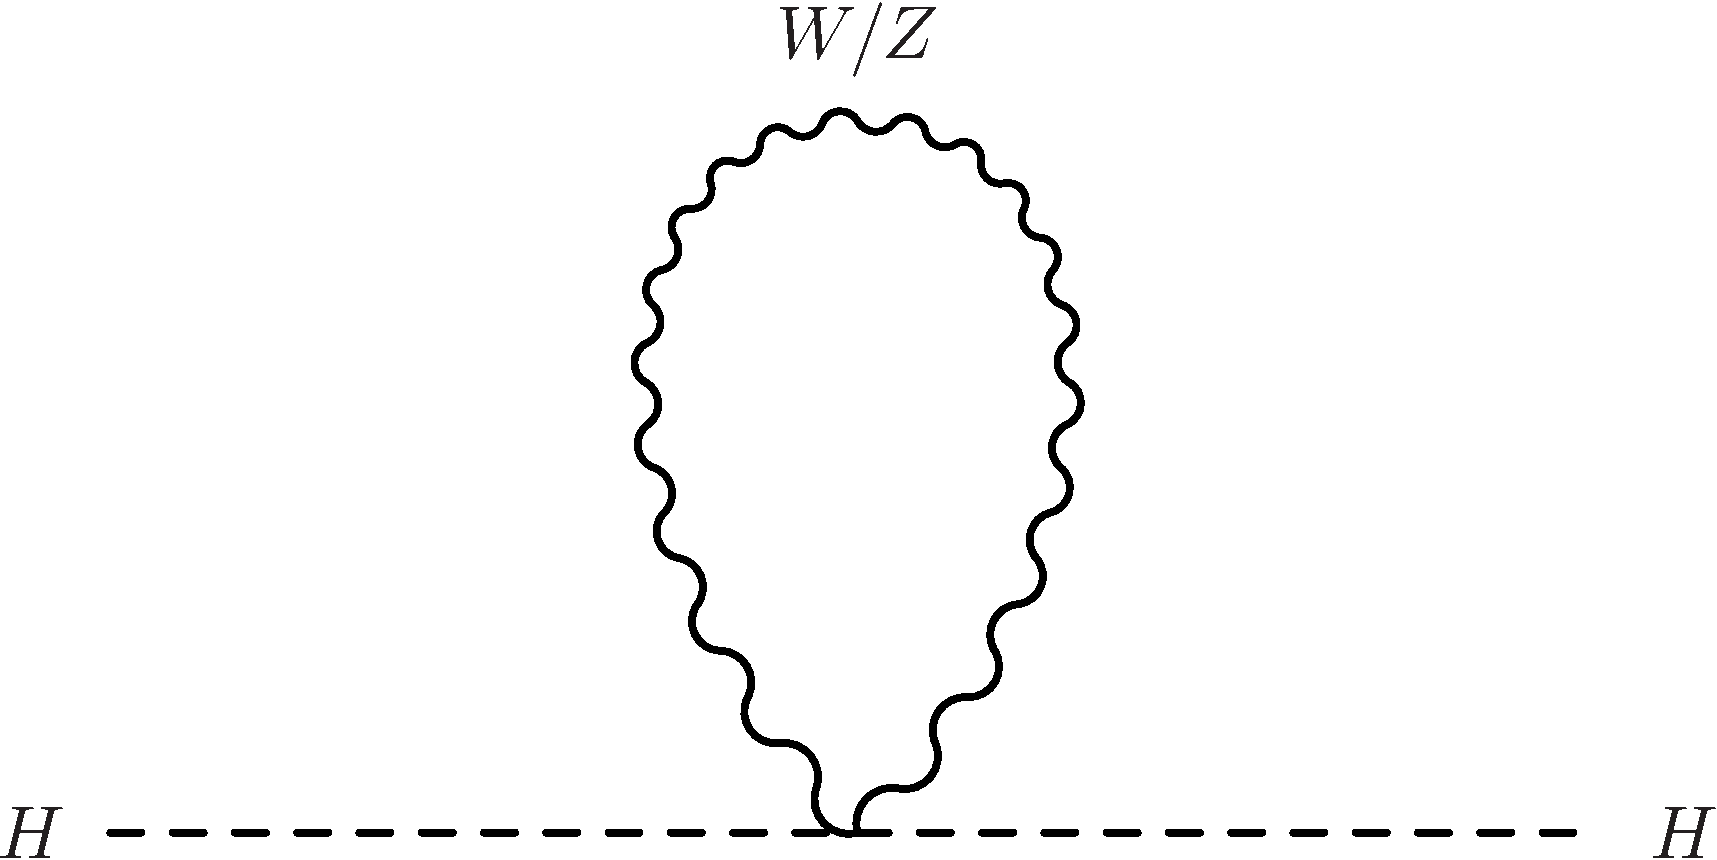
\includegraphics[width=0.3\textwidth]{\chtwo/HiggsLoop1.pdf}}
 \subfigure[]{\label{fig:HiggsLoop_c}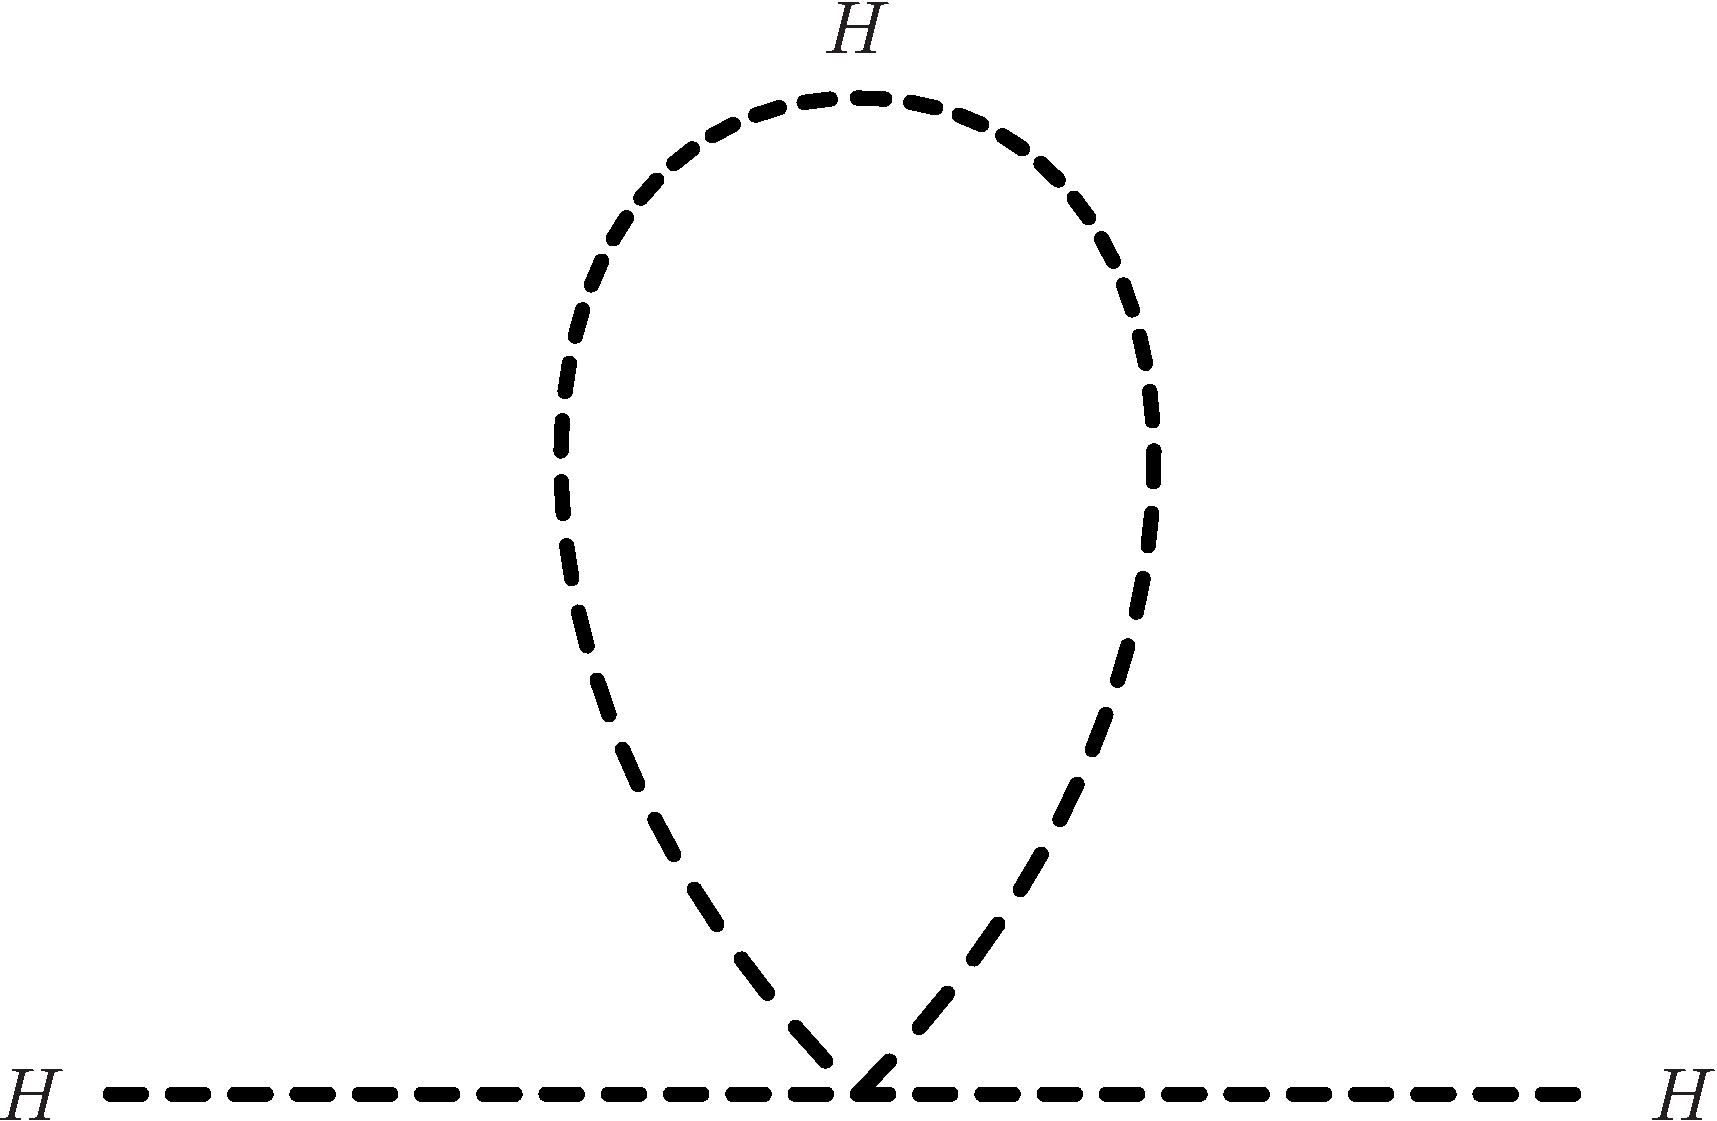
\includegraphics[width=0.3\textwidth]{\chtwo/HiggsLoop2.pdf}} 
 \caption{Radiative corrections to the Higgs squared mass parameter $M^2_\PH$ due to: (a) Yukawa coupling with the top quark; (b) gauge boson loop; (c) Higgs quartic self-interaction.}
 \label{fig:HiggsLoop}
\end{figure}

Many extensions of the SM suggest new physics at the TeV scale to address the hierarchy problem, providing more ``natural'' options.
Models of \textit{supersymmetry}~\cite{PhysRevD.24.1681,Casas:1994qy} introduce a new heavy scalar called \textit{stop} as a \textit{superpartner} of the SM top quark,
which produces loop corrections to the Higgs-boson mass that cancel out those of the top quark.
Non-supersymmetric models have also been proposed, which predict heavier partners to the top quark.
%In \textit{Little Higgs} models (Section~\ref{subsec:composite}), several heavy top quark partners (also called vector-like quarks) are introduced which cancel the quadratic divergence.
Another possibility to address the hierarchy problem is to assume the Higgs boson to be a composite particle as in the \textit{composite Higgs} models (Section~\ref{subsec:composite}),
rather than an elementary particle as predicted in the SM. %In these composite Higgs models, a Higgs boson may have decays as predicted by the SM. 

\subsection*{Dark matter and dark energy}

Several cosmological observations have demonstrated that the standard model only describes 5\% of the total energy content of the Universe.
First, the measured orbital velocities of stars around their galaxy center is incompatible with the observed matter density of the galaxy~\cite{DarkMatterRubin,Iocco:2015xga}.
In particular, assuming the gravitational mass is due to only visible matter, stars far from the center of galaxies have much higher velocities than expected. % (Fig.~\ref{fig:DarkMatter}).
The easiest way to account for this discrepancy is to postulate the existence of another kind of matter, called \textit{dark matter}, that does not interact through electromagnetic or strong interactions.
%\begin{figure}[!htb]
 %\centering
 %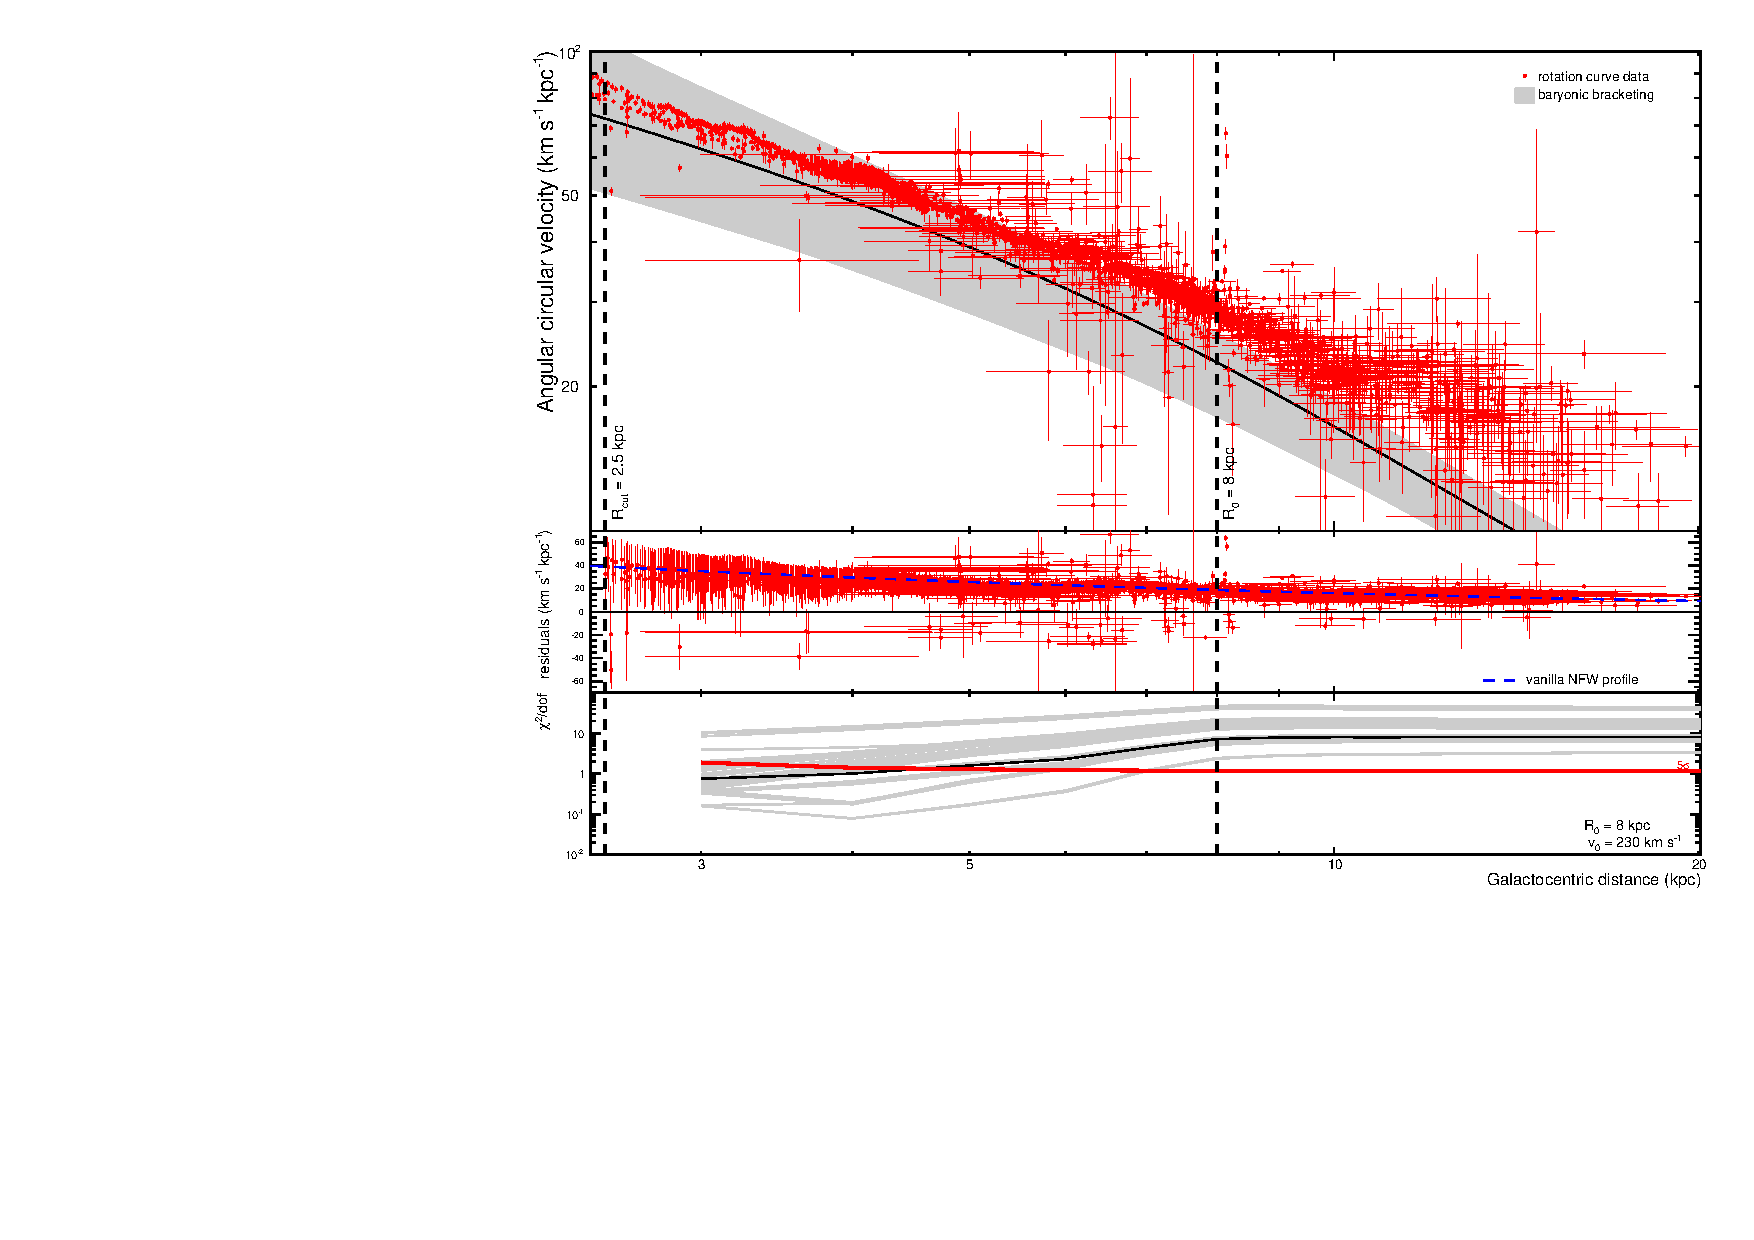
\includegraphics[width=0.6\textwidth]{\chtwo/wc_fit.pdf}
 %\caption{Measured rotation curve of the Milky Way representing the orbital velocities of visible stars or gas in that galaxy as a function of their radial distance from that galaxy's center. The contribution from visible matter is represented by the black line with its 1$\sigma$ uncertainty (grey band). The data strongly disfavor baryons as the sole contribution to the galactic mass budget~\cite{Iocco:2015xga}.}
 %\label{fig:DarkMatter}
%\end{figure}
A second major result in cosmology is the discovery that the Universe is in accelerated expansion: it was measured that on average galaxies recede from each other and that this expansion rate increases with the distance.
Such a feature cannot be achieved with usual particles or with dark matter, but rather a new type of energy with a negative pressure, called \textit{dark energy}, has to be added to the Universe content.
To account for the experimental observations, dark matter and dark energy have been measured at percent-level uncertainty to compose respectively 26\% and 69\% of the total Universe content~\cite{Ade:2015xua}, but their fundamental nature remains nowadays a mystery.
The most widely accepted hypothesis on the form for dark matter is that it is composed of \textit{weakly interacting massive particles} (WIMPs) that interact only through the gravitational force and an unknown force which is as weak as or weaker than the SM weak force.
The search from the point of view of experimental and theoretical dark matter hunting is one of the major efforts in particle physics.
There are two fronts: direct searches in cosmic rays by underground experiments, and searches at hadron colliders, where dark matter would be produced as a pair of neutral particles that may be predicted by different models.
%In the case of supersymmetry, dark matter is incarnated by neutralinos ($\tilde{\chi}^0$), often called Weakly Interacting Massive Particles or WIMP's, in processes such as 
%\begin{equation*}
%p p \to X \to \tilde{\chi}^0 \tilde{\chi}^0
%\end{equation*}
No dark matter particle has been conclusively identified by any of these experiments.

\subsection*{Gravitational force}

The standard model does not include the fourth fundamental interaction, the gravitational force.
In fact, the gravitational force is by many aspects very different from the three other forces, and establishing a common framework to describe both raises several challenges.
In the decades after the discovery of general relativity, it was realized that general relativity is incompatible with quantum mechanics.
It is possible to describe the gravitational force in the framework of quantum field theory like the other fundamental forces, such that the attractive gravitational force arises due to exchange of virtual spin-2 \textit{gravitons}, in the same way as the electromagnetic force arises from exchange of virtual photons. The theory arising from this approach is known as \textit{quantum gravity}.
%Moreover, whereas the strong, weak and electromagnetic forces have similar strengths at the electroweak scale, gravity is $10^{24}$ times weaker and becomes only appreciable for energies around the Planck scale.
This theory is known not to be renormalizable, as the loop corrections including a graviton induce divergencies that cannot be reabsorbed through the renormalisation procedure, as opposed to the electroweak and chromodynamics quantum theories. Thus, quantum gravity cannot be used to make meaningful physical predictions.
%Thus, a more complete theory of quantum gravity is required.
Moreover, quantum gravitational effects are only expected to become apparent near the Planck scale, a scale far smaller in distance (equivalently, far larger in energy) than what is currently accessible at high energy particle accelerators.
Several theoretical approaches to the problem of quantum gravity have been proposed, the most popular one being \textit{string theory}~\cite{StringTheory}.
%and \textit{loop quantum gravity}~\cite{Rovelli:2011eq}.

It has to be noted that most of these approaches only attempt to describe the quantum behavior of the gravitational field and should not be confused with the objective of unifying all fundamental interactions into a single mathematical framework. However, the present understanding of the gravitational force would aid further work towards unification.
%A theory of quantum gravity that is also a grand unification of all known interactions is sometimes referred to as the \textit{theory of everything}.

%matter-antimatter asymmetry
%number of parameters
%number of flavors
%neutrino oscillations
  
%\section{Theories of new physics}
  \section{Theories of new physics}
\label{sec:BSMintro}

The standard model of particle physics has been very successful in describing observations. 
However, as explained in the previous section, this framework leaves several unanswered fundamental questions.
Many extensions to the standard model have been proposed that attempt to address the open issues and to achieve a more fundamental theory
that could explain the entirety of current phenomena.
These new theoretical developments are referred to as \textit{beyond standard model} (BSM) theories.
In this section, three specific BSM scenarios are reviewed, which are of particular interest because of their highly predictive features.
Specifically, with the aim of addressing the hierarchy problem of the SM, they predict the existence of new resonances with masses in the TeV range,
which can be produced at hadron colliders.
Furthermore, since the new resonances can decay into pairs of well-known standard model particles, their existence and properties can be directly probe by collider experiments.
In particular, the decay modes into a pair of electroweak bosons \PW, \PZ or \PH, can provide striking signatures, as new techniques have been developed by the experiments to efficiently reconstruct the decay and mass of the bosons in the final state.

%%%%%%%%%%%%%%%%%%%%%%%%%%%%%%%%%%%%%%%%%%%%
\subsection{Warped Extra dimensions}\label{subsec:graviton}
%%%%%%%%%%%%%%%%%%%%%%%%%%%%%%%%%%%%%%%%%%%%

A class of theories beyond the standard model are those postulating the existence of new compactified spatial dimensions.
They attempt to explain the apparent weakness of gravity by assuming that SM particles are confined in a (3+1)-dimensional hypersurface called \textit{3-brane},
as opposed to gravity which is allowed to propagate in a (4+n)-dimensional \textit{bulk}.
In this scenario, the strength of gravity is diluted in the extra dimensions (thereby weakening our perception of gravity), while the other fundamental forces would not.

The basic idea comes from the so-called \textit{large extra dimensions} scenario proposed by Arkani-Hamed, Dimopoulos and Dvali (ADD model)~\cite{ArkaniHamed:1998rs}.
If spacetime has 4+$n$ dimensions, then the effective 4-dimensional (reduced) Planck scale, $\bMPl = \MPl/\sqrt{8\pi}$,
is determined by the fundamental (4+$n$)-dimensional Planck scale, $M_*$, and the geometry of the extra dimensions:

\begin{equation}\label{eqn:WED_1}
\bMPl^2 = V_nM^{n+2}_* \simeq R^nM^{n+2}_*,
\end{equation}

\noindent where $V_n$ is the volume of the $n$-dimensional compactified space and $R$ its radius.
The hierarchy problem is thus eluded if $M_* \sim 1\TeV$, which turns into a condition on the size $R$ of the extra dimensions.
Assuming $n = 1$, one can solve Eq.~\ref{eqn:WED_1} and obtain $R \sim 10^8\unit{m}$.
This is a scale of the order of the Earth-Sun distance, over which we know that the $1/r^2$ Newton's law of gravitational attraction works very well. Thus, $n = 1$ is excluded.
For $n = 2$, one obtains $R \sim 100\mum$ or $R^{-1} \sim 10^{-4}$\unit{eV}, which is close to the limit of current table top experimental searches for deviations from the Newton's law~\cite{Hoyle:2004cw}. 

The purpose of this model was to eliminate the hierarchy problem, i.e. to remove the large ratio between the weak scale $v$ and the true fundamental scale \bMPl, hence the requirement $M_* \sim 1\TeV$.
However, it introduces a new hierarchy, namely that between the compactification scale $\mu_c = 1/R$ and $v$.
Thus, the ADD really only trades one large ratio for another and does not really eliminate the hierarchy problem.
An alternative solution, represented by the so-called \textit{warped extra dimensions} (WED) scenario, has been proposed by Randall and Sundrum (RS)~\cite{Randall:1999ee}.

\begin{wrapfigure}{R}{0.4\textwidth}
 \centering
 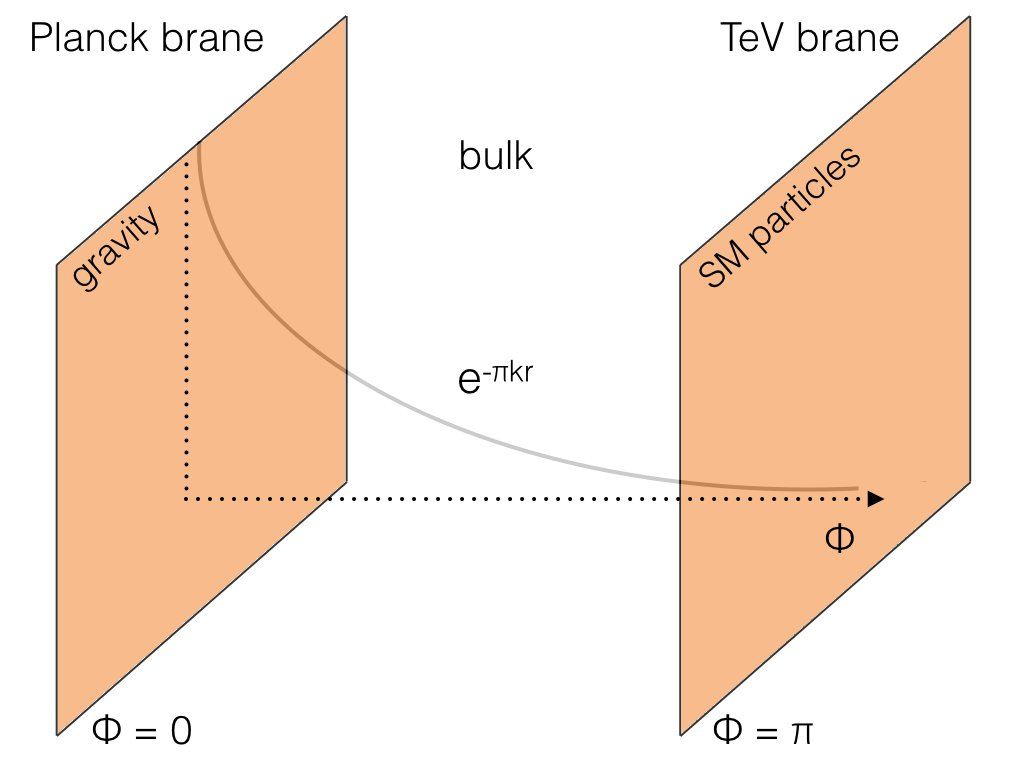
\includegraphics[width=0.35\textwidth]{\chtwo/RS1model.png}
 \caption{Set-up of the five dimensions in the RS model. The \textit{Planck} and \textit{TeV} branes are the 4-dimensional boundaries of the extra dimension $\phi$ compactified in an interval $[0,\pi]$.}
 \label{fig:WED}
\end{wrapfigure}

The basic RS model, referred to as RS1, assumes the existence of only one extra dimension with size $r_c$. This fifth, extra dimension is labelled by the coordinate $\phi \in [-\pi,\pi]$,
such that it can be described by a line segment between two 4-dimensional branes (or 3-branes), known as the \textit{Planck} and \textit{TeV} brane, located, respectively,
at the $\phi = 0$ and $\phi = \pi$ boundary of the fifth dimension (Fig.~\ref{fig:WED}).
In the simplest version of the RS model, it is assumed, like in the ADD case, that the SM fields live on the \textit{TeV} brane, while gravity lives everywhere.
The \textit{Planck} brane is where gravity is a relatively strong force.
The classical action describing the above set-up is given by the sum of the gravitational action in the bulk, $\mathcal{S}_{gravity}$, and on the two branes, $\mathcal{S}_{TeV}$ and $\mathcal{S}_{Planck}$,

\begin{equation}\label{eqn:WED_2}
\begin{gathered}
\mathcal{S} = \mathcal{S}_{gravity} + \mathcal{S}_{TeV} + \mathcal{S}_{Planck}, \\
\mathcal{S}_{gravity} = \int d^4x \int_{-\pi}^{+\pi} d\phi\sqrt{-G}{-\Lambda+2M^3_*R}, \\
\mathcal{S}_{TeV} = \int d^4x\sqrt{-G(x^\mu,\phi=\pi)}\Lambda, \\
\mathcal{S}_{Planck} = \int d^4x\sqrt{-G(x^\mu,\phi=0)}\Lambda.
\end{gathered}
\end{equation}

In the above equation, $G$ is the 5-dimensional metric $G_{\mu\nu}$, $\Lambda$ a cosmological constant, and $R$ the 5-dimensional Ricci tensor.
By requiring a solution of the 5-dimensional Einstein's equation for the above action that respects the 4-dimensional Poincar\'{e} invariance in the $x^\mu$ coordinates,
one finds that the 5-dimensional metric must take the form 

\begin{equation}\label{eqn:WED_3}
ds^2 = e^{-2\sigma(\phi)} \eta_{\mu\nu}dx^\mu dx^\nu + r^2_cd\phi,
\end{equation}

\noindent where $\eta_{\mu\nu} = \mathrm{diag}(1,-1,-1,-1)$ is the usual Minkowski metric and $\sigma(\phi)$ is some a priori unknown function.
This type of geometry is called ``non-factorizable'', because the metric of the 4-dimensional subspace is $\phi$-dependent.
Solving the 5-dimensional Einstein's equations provides a unique solution for $\sigma(\phi)$:

\begin{equation}\label{eqn:WED_4}
\sigma(\phi) = \sqrt{\frac{-\Lambda}{24M^3_*}} \equiv r_c|\phi|k,
\end{equation}

\noindent where $k$ is referred to as the \textit{curvature factor}.
By plugging the solution back into the original action and integrating out the extra dimension $\phi$, one finds that the 4-dimensional Planck mass is given by

\begin{equation}\label{eqn:WED_5}
\bMPl = \frac{M^3_*}{k}(1 - e^{-2\pi kr_c}).
\end{equation}

%\noindent where the term $e^{-2\pi kr_c}$ is usually called the \textit{warp factor}.
It is assumed that $k \sim M_* \sim \bMPl$ in order to avoid producing strong hierarchy between the mass scales of the theory.
However, the electroweak energy scale $v$ or any physical mass $m$ in the \textit{TeV} brane is exponentially suppressed compared to the 5-dimensional energy $v_0$ or mass $m_0$:

\begin{equation}\label{eqn:WED_6}
m = e^{-\pi kr_c}m_0 \, , \qquad\qquad v = e^{-\pi kr_c}v_0.
\end{equation}

This means that by taking $v_0$ of the order of the 5-dimensional fundamental mass scale $M_*$, the separation between the Planck mass and electroweak scales
is produced by the metric when $kr_c \sim 11$ (small hierarchy). Such factor indeed would already suppress a parameter with value of order $10^{18}\GeV$ to only 1\TeV.
The hierarchy is thus naturally established by the warp factor $e^{-\pi kr_c}$.
This Planck-electroweak hierarchy explanation is the most celebrated achievement of WED scenarios.

A distinctive novel feature of the RS scenario is the existence of a so-called tower of Kaluza--Klein (KK) excitations of a spin-2 field, the KK graviton, arising from tensor fluctuations 
around the 4-dimensional part of the metric. Scalar fluctuations around the fifth extra dimension give rise to a spin-0 field called \textit{radion}.
Massive graviton excitations appear, with 4-dimensional effective masses given by

\begin{equation}\label{eqn:WED_7}
m_G^{(n)} = kx_ne^{-\pi kr_c},
\end{equation}

\noindent where $x_n$ is the $n$-th root of the Bessel function $J_1$. These masses are of order of a TeV, so that Kaluza-Klein gravitons can be detected as massive resonances in collider experiments. 
The zero-mode of the graviton field corresponds to the mediator of gravitational interaction, and its wave function is highly peaked at $\phi = 0$. Gravity is thus localized on the \textit{Planck} brane, while on the \textit{TeV} brane we feel only the tail of the graviton wave-function. %So in the RS model the reason of the weakness of gravity is that it is localized far away from where we live.

The coupling of an excited graviton to matter is described by the Lagrangian

\begin{equation}\label{eqn:WED_8}
\mathcal{L} = - \frac{1}{\Lambda_\pi}T^{\mu\nu}\sum_{n>0}h^{(n)}_{\mu\nu},
\end{equation}

\noindent where $T^{\mu\nu}$ is the energy-momentum tensor of the matter field, $h^{(n)}_{\mu\nu}$ is the $n$-th excitation of the graviton,
and $\Lambda_\pi = \bMPl e^{-\pi kr_c}$ is of order of TeV.
It is interesting to note that this model has only two free parameters: the mass of the first (lightest) KK-graviton excitation, $m_1$, and the ratio $\tilde{k} \equiv  k/\bMPl$, which controls the widths of the new resonances:

\begin{equation}\label{eqn:WED_9}
\Gamma_n = \rho m_n x^2_n\tilde{k}^2,
\end{equation}

\noindent where $\rho$ is a constant depending on the number of open decay channels.
The RS model in its simplest form is thus highly predictive.\\

In the original RS1 model the SM matter is localized on the \textit{TeV} brane, as the Higgs field.
A well-motivated extension of the original RS1 model explored an alternative scenario, in which 
SM fields propagate in the warped bulk, except for the Higgs field which is required on the \textit{TeV} brane to avoid hierarchy.
This extension is referred thereafter as the \textit{bulk scenario}~\cite{Agashe:2007zd,Fitzpatrick:2007qr}.
Similarly to the KK-graviton excitations, in the bulk scenario a KK expansion is applied to each SM field.
The zero-mode of each KK tower represents the correspondent SM particle.
The first and second generation fermions are localized near the \textit{Planck} brane, leading to the the small Yukawa couplings to the Higgs field which is localized on the \textit{TeV} brane.
Similarly, the top quark can be localized near the \textit{TeV} brane to account for its large Yukawa coupling.
In the original RS1 scenario all the particles are localized on the \textit{TeV} brane, therefore the strength of the couplings between KK-graviton and SM particles are democratic. 
As a consequence, the RS gravitons are produced via both \qqbar annihilation and gluon fusion processes.
In the bulk scenario, couplings of KK gravitons to light fermions are highly suppressed since, as mentioned above, KK gravitons are localized near the \textit{TeV} brane, whereas light fermions are localized near the \textit{Planck} brane. As a result, \qqbar annihilation at hadron collider for KK graviton production is negligible in this case.
In contrast, SM gluons have a flat localization in the bulk, so that the coupling of gluons to KK gravitons and hence KK graviton production via gluon fusion is dominant.
Furthermore, decays of KK graviton into top quarks and Higgs bosons are enhanced due to their profile being near the \textit{TeV} brane, resulting in couplings to KK gravitons (which are also localized there) being only $\sim\TeV$-suppressed just like in the original RS1 model (Eq.~\ref{eqn:WED_8}).
Another crucial point of the bulk scenario is that before symmetry-breaking, the \PW and \PZ gauge bosons start out with flat localization in the bulk. %and the Higgs starts out with a delta function wave-function on the brane.
However, after symmetry-breaking, the gauge bosons eat a Higgs, and their wave functions are still mostly flat in the bulk but fall sharply near the brane.
Thus, in the bulk scenario, branching fractions for decays into pair of vector bosons are the same size as those for decays into Higgs bosons or top quarks.
The branching fractions for the different decay modes of the graviton in both the bulk and RS1 scenarios are shown in Fig.~\ref{fig:GrBR} as a function of the graviton mass.
It can also be shown that in RS1 scenario the graviton decays preferentially to transverse polarized vector bosons, whereas in the bulk scenario it decays preferentially to longitudinally polarized modes, making those two benchmarks an excellent framework to study the sensitivity of the vector boson identification techniques used at the collider experiments to the polarization (Chapter~\ref{ch:vtagging}).

\begin{figure}[!htb]
\centering
\subfigure[]{\label{fig:GrBR_a}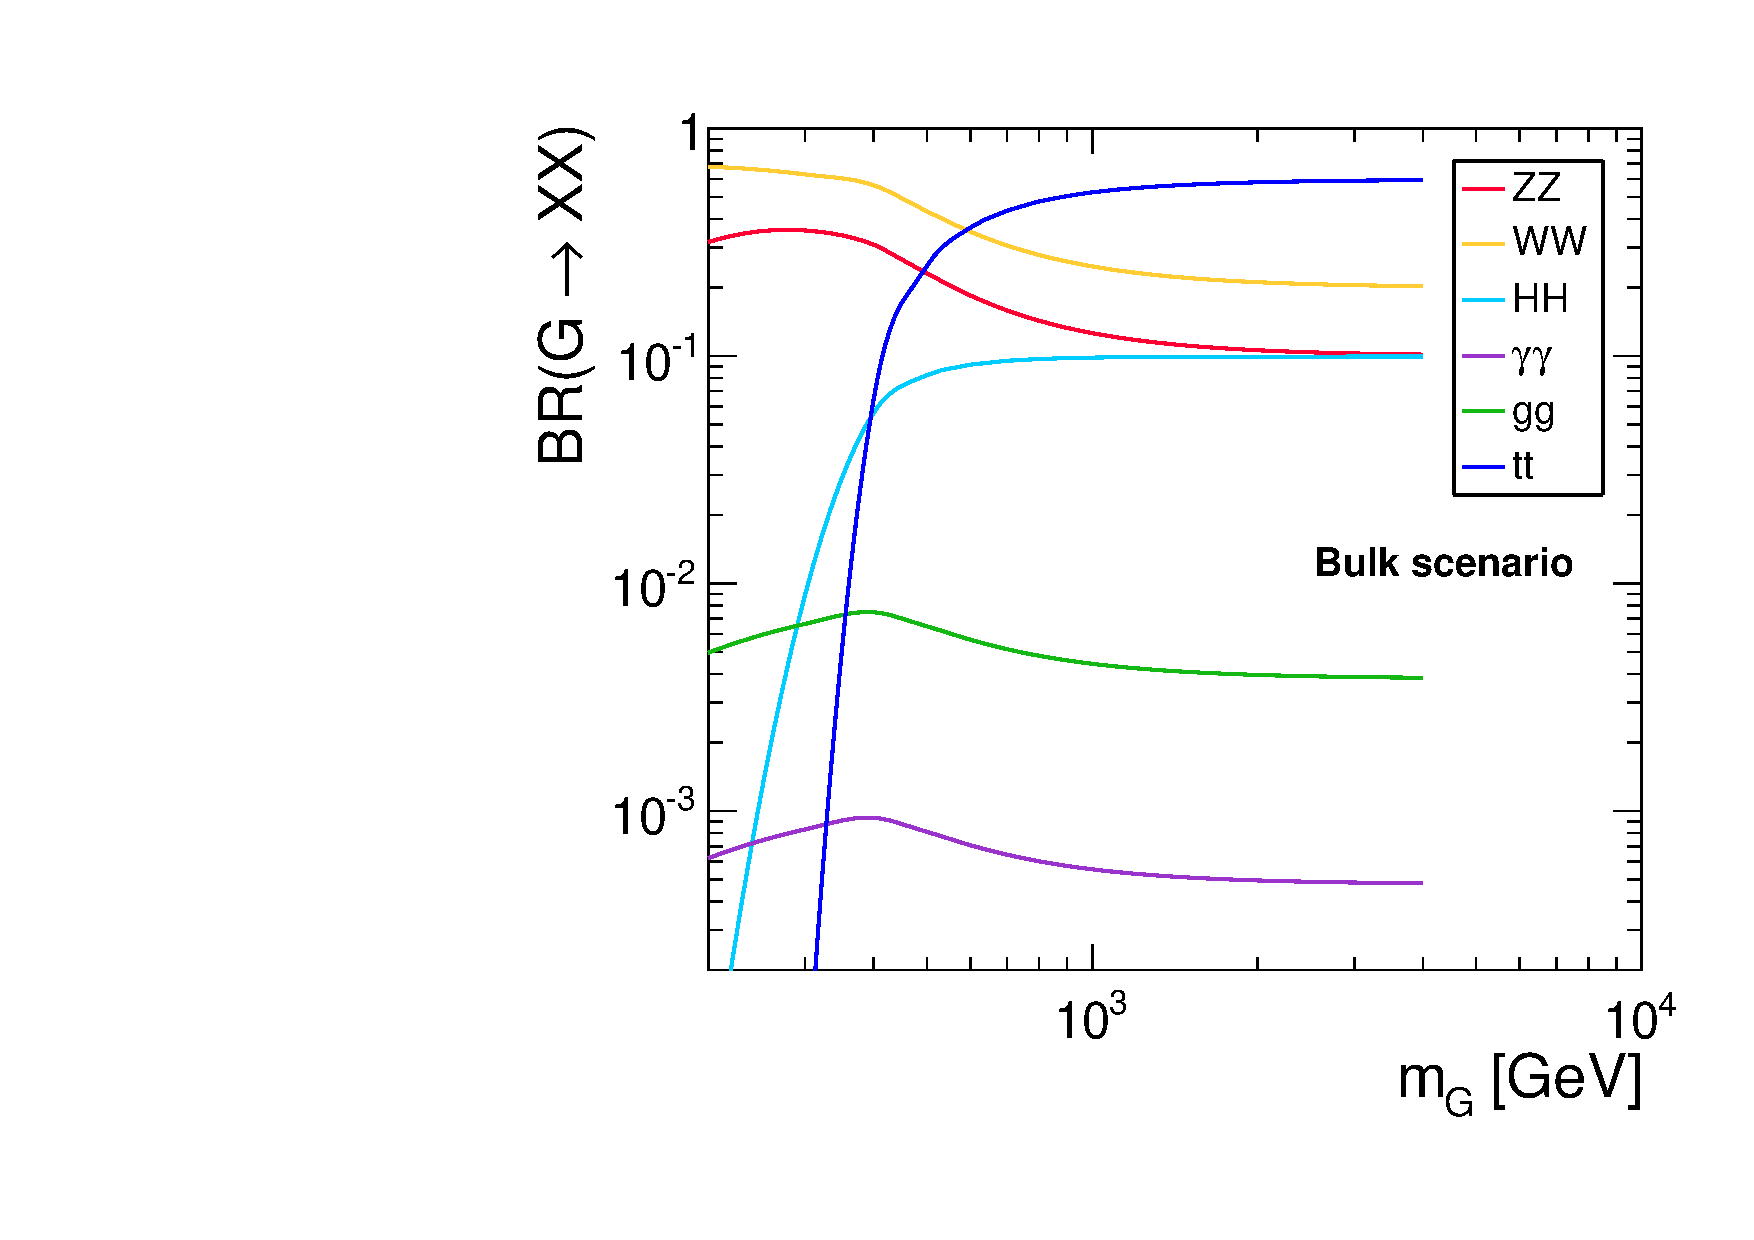
\includegraphics[width=0.45\textwidth]{\chtwo/brs-bulkg.pdf}}
\subfigure[]{\label{fig:GrBR_b}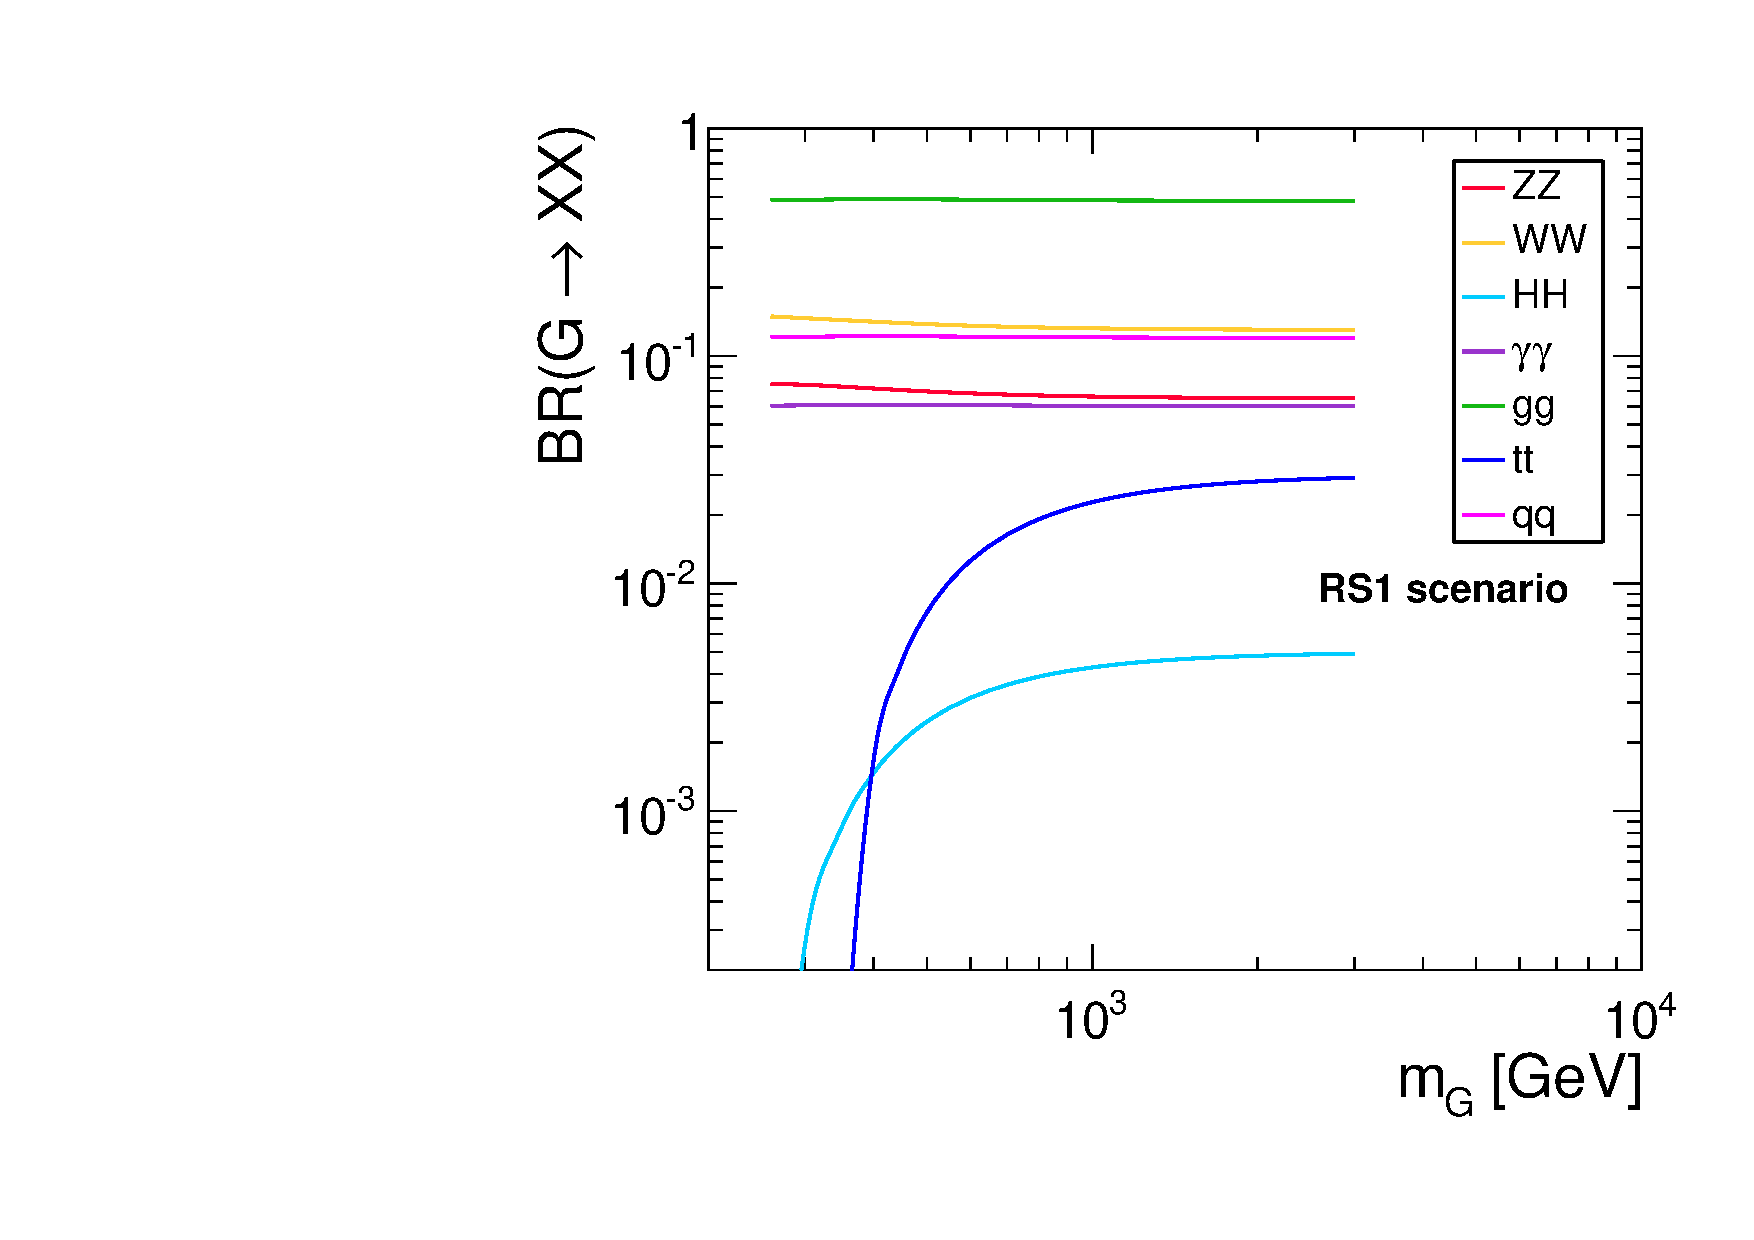
\includegraphics[width=0.45\textwidth]{\chtwo/brs-rs1.pdf}}
\caption{Branching fractions for the different decay modes of the graviton in the (a) bulk and (b) RS1 scenarios, as a function of the graviton mass.}
\label{fig:GrBR}
\end{figure}

%%%%%%%%%%%%%%%%%%%%%%%%%%%%%%%%%%%%%%%%%%%%
\subsection{Compositeness}\label{subsec:composite}
%%%%%%%%%%%%%%%%%%%%%%%%%%%%%%%%%%%%%%%%%%%%

One of the approaches to the hierarchy problem compatible with observations is based on the assumption that the Higgs boson is a composite particle, a bound state of more fundamental constituents held together by a new strong force.
In composite Higgs models~\cite{Composite0,Composite1,Composite2}, $\Lambda$ is the energy scale where the composite nature of the Higgs boson becomes important, which roughly coincides with the confinement scale of the new strong interaction. Thus, the solution to the hierarchy problem is that there is no elementary scalar, and beyond $\Lambda$ an experiment becomes sensitive to the underlying ``partons'' that compose the Higgs boson. 
However, precision electroweak data rule out new strong interactions at scales below about 10\TeV.
One key question is therefore the lightness of the Higgs boson with respect to such scale.

By comparing with the QCD sector, one observes that the strong coupling scale is $\Lambda_\mathrm{QCD} \sim \mathcal{O}(300\MeV)$, whereas most bound states, such as the $\rho$ meson and proton, are at least as heavy as this.
However, a counter-example in QCD is given by the existence of the pions, which are all lighter than $\Lambda_\mathrm{QCD}$, although only by a $\mathcal{O}(1)$ factor.
The reason for the pions to be appreciably lighter than the other QCD bound states is found in the chiral perturbation theory. 
In fact, the pions represent the Goldstone bosons of the spontaneously broken $SU(2)_L \times SU(2)_R$ flavor symmetry coming from chiral rotations of the up and down quarks. 
The spontaneous symmetry breaking of the flavor symmetry into the vectorial isospin subgroup $SU(2)_V$, is induced by a non-perturbative QCD vacuum state, characterized by a non-vanishing quark condensate $\langle \bar{q}^a_L q^b_R \rangle \sim \delta^{ab}\Lambda^3_\mathrm{QCD}$.
However, because of the non-vanishing and differing masses of the quarks, the $SU(2)_L \times SU(2)_R$ is only an approximate symmetry, and therefore the pions are not massless, but have small masses, so that they are \textit{pseudo-Goldstone bosons}.

In composite Higgs models, a similar structure is assumed, where the Higgs is a pseudo-Goldstone boson of some symmetry with strong coupling scale $\Lambda \approx 4\pi f$,
where $f$ is the scale at which the symmetry is spontaneously broken.
The main idea is that the Higgs mass parameter is protected against quadratic quantum corrections up to the compositeness scale because it is a pseudo-Goldstone boson. 
Above the scale of compositeness, it is simply not an elementary scalar.
Furthermore, the pseudo-Goldstone nature of the Higgs is an explanation for why the Higgs mass is so much lighter than the other bound states in the strongly coupled sector.

Such models start with a large global symmetry group $G$, analogous to the ``large'' $SU(2)_L \times SU(2)_R$ global symmetry of low energy QCD.
The strong dynamics spontaneously breaks $G$ to a subgroup $H$, similarly to the QCD chiral symmetry breaking $SU(2)_L \times SU(2)_R \to SU(2)_V$.
In a minimal composite Higgs model $G = SO(5) \to H = SO(4)$.
The SM electroweak group $SU(2)_L \times U(1)_Y$ is a subgroup of $H$, thus introducing a preferred orientation in the coset space SO(5)/SO(4) with respect to the global SO(4).
In this way, the electroweak scale $v$ is distinct from the $G \to H$ symmetry breaking scale $f$. The parameter $\xi = (v/f)^2$ is introduced to characterize this separation of scales and to quantify the degree of vacuum misalignment.
In a theory with little hierarchy $\xi \sim 1$, while a small amount of fine-tuning can give rise to $\xi \ll 1$. In particular, compatibility with the constraints coming from electroweak precision tests and Higgs coupling measurements generically implies $\xi \lesssim 0.2$. This bound places the scale $f$ at about 1\TeV, resulting in a strong coupling scale $\Lambda \approx 4\pi f \sim 10\TeV$.
Such large value results in a large one-loop contribution to the Higgs mass parameter (Eq.~\ref{eqn:HiggsCorr}), so that a generic composite Higgs set up still requires some tuning between the $v$ and $f$ scales.
One way to generate a ``little hierarchy'' is through the mechanism of \textit{collective symmetry breaking} as in \textit{Little Higgs} (LH) scenarios~\cite{Han:2003wu,Perelstein:2005ka,Schmaltz:2005ky,Arkani:2002LH}, which is now a key ingredient in composite Higgs models.
The main idea of this approach is that one can separate the scales $v$ and $f$ by introducing new particles, which cancel the quadratic divergences at one-loop order. 
In particular, the quadratic divergence induced by the SM gauge boson loops are canceled by the quadratic divergence induced by heavy gauge bosons at one loop level.
Heavy fermionic states are also introduced, which couple to the Higgs field such that the one-loop quadratic divergence induced by the top-quark Yukawa coupling to the Higgs boson is canceled.
Furthermore, extra Higgs fields exist as the Goldstone boson multiplets from the global symmetry breaking.
%In Little Higgs models, instead of a simple global group $G$ a direct product of two (or more) groups $G_1 \times G_2 \times \dotsc$ is considered so that its breaking has a collective nature.
%The models then contain additional gauge bosons at the TeV scale that produce the necessary cancellations to the one-loop quadratic divergence.
%It implies that any non-vanishing quantum contribution to the Higgs mass parameter must necessarily be proportional to a product of all the gauge coupling constants corresponding to the different $G_i$ factors.
%Thus, setting any one of the coupling constants to zero must result in a vanishing contribution.
%The extended gauge group $G_1 \times G_2 \times \dotsc$ of the LH models is typically broken down to the SM $\mathrm{SU(2)_L \times U(1)_Y}$ at a scale $f$ by the same condensates that break $G \to H$.
%The models then contain additional gauge bosons at the TeV scale. In the mass eigenbasis, the vanishing of the one-loop quadratic divergence can be understood as a result of a cancellation between the SM bow tie diagrams and their counterparts involving the TeV-scale bosons. 
This is achieved by enlarging the simple global group $G$ and embedding two parallel global symmetries $G_1 \times G_2$, such that $G \supset G_1 \times G_2 = [SU(2)_1 \times U(1)_1] \times[SU(2)_2 \times U(1)_2]$.
A specific implementation, called the \textit{littlest Higgs}~\cite{Arkani:2002LH}, starts with the global symmetry $G$ = SU(5), which is spontaneously broken down at the scale $\Lambda$ to its subgroup $SO(5)$ via a vacuum expectation value of order $f$. At the same time, the gauge symmetry $[SU(2) \times U(1)]^2$ is also broken into $[SU(2)_L \times U(1)_Y]$, identified as the SM gauge group.
The global symmetry breaking leaves 14 massless Goldstone bosons, which become the longitudinal components of the $\mathrm{W}^{\prime\pm}$  and $\PZpr$ gauge bosons associated with the broken gauge groups, giving them masses of the order $f$:

\begin{equation}\label{eqn:LHvprimeMass}
M(\mathrm{W}^{\prime\pm}) \simeq M(\PZpr) = \frac{g}{\sin2\theta}f,
\end{equation}

\noindent where $\theta$ is given by the gauge couplings of the two broken $SU(2)$ groups: $\tan\theta = g_1/g_2$.
The partial decay widths are computed using the formalism of Feynman rules:

\begin{equation}
\begin{aligned}
\Gamma(\mathrm{W}^{\prime\pm} \to \ell\nu) & \simeq \Gamma(\PZpr \to \ell\ell) & = \frac{g^2\cot^2\theta}{96\pi}M\\
\Gamma(\mathrm{W}^{\prime\pm} \to \mathrm{q}\bar{\mathrm{q}}^\prime) & \simeq \Gamma(\PZpr \to \qqbar) & = \frac{g^2\cot^2\theta}{32\pi}M\\
\Gamma(\mathrm{W}^{\prime\pm} \to \PW\PH) & \simeq \Gamma(\PZpr \to \PZ\PH) & = \frac{g^2\cot^22\theta}{192\pi}M\\
\Gamma(\mathrm{W}^{\prime\pm} \to \PW\PZ) & \simeq \Gamma(\PZpr \to \PW\PW) & = \frac{g^2\cot^22\theta}{192\pi}M
\end{aligned} 
\end{equation}

\noindent where $M$ is the mass of the \PVpr triplet given by Eq.~\ref{eqn:LHvprimeMass}.
Summing over all the quark and lepton channels results in a total width

\begin{equation}
\Gamma_\mathrm{tot} = \frac{g^2}{96\pi}(\cot^22\theta + 24\cot^2\theta)M.
\end{equation}

One can immediately observe that the fermionic decay modes dominate for $\cot\theta \geq 1/2$, while bosonic decay modes become significant only below this value.
However, since the \PVpr resonances are produced mainly via the Drell-Yan process $\qqbarpr \to \PVpr$, one should notice that the production cross section would be at the same time suppressed for the enhanced bosonic channels.
Thus, the interactions of the new predicted particles is described within these theories, and detailed predictions of their properties are made.
Furthermore, they provide distinct signatures that can be searched for at the hadron collider.

%%%%%%%%%%%%%%%%%%%%%%%%%%%%%%%%%%%%%%%%%%%%
\subsection{Heavy vector triplet}\label{subsec:hvt}
%%%%%%%%%%%%%%%%%%%%%%%%%%%%%%%%%%%%%%%%%%%%

New heavy spin-1 resonances are predicted by several extensions of the standard model, such as the Composite Higgs and Little Higgs models described in the previous section.
A model-independent strategy has been proposed in Ref.~\cite{Pappadopulo:2014qza} to study these resonances, based on a simplified phenomenological Lagrangian, which reproduces a large class of explicit models.
The main reason for introducing a simplified model is that the experimental searches for new resonances are typically not sensitive to all the details and the free parameters of the chosen benchmark model, but only to those parameters or combinations of parameters that control the mass of the resonance and the interactions involved in its production and decay. Therefore one can employ a simplified description of the new phenomena, where only the relevant couplings and mass parameters are retained. In turn, the experimental results expressed in terms of the phenomenological parameters can be easily translated into the free parameters of any explicit model by computing the phenomenological/explicit parameter relations.\\

In this approach, a new real vector in the $\mathrm{SU(2)_L}$ representation is introduced in addition to the SM fields, describing one charged and one neutral heavy spin-1 particle (heavy vector triplet or HVT) with the charge eigenstate fields given by

\begin{equation}\label{eqn:HVT_1}
V^\pm_\mu = \frac{V^1_\mu \mp iV^2_\mu}{\sqrt{2}} \, \qquad\qquad V^0_\mu = V^3_\mu.
\end{equation}

The dynamics of the new vector is described by a simple phenomenological Lagrangian

\begin{equation}\label{eqn:HVT_2}
\begin{split}
\mathcal{L}_V = & -\frac{1}{4}\mathcal{D}_{[\mu}V^a_{\nu]}\mathcal{D}^{[\mu}V^{\nu]a} + \frac{m^2_V}{2}V^a_\mu V^{\mu a}\\
 & + ig_Vc_HV^a_\mu H^\dag\tau^a\overleftrightarrow{\mathcal{D}}^\mu H + \frac{g^2}{g_V}c_FV^a_\mu J^{\mu a}_F\\
 & + \mbox{extra terms}
 %& + \frac{g_V}{2}c_{VVV}\epsilon_{abc}V^a_\mu V^b_\nu\mathcal{D}^{[\mu}V^{\nu]c} + g^2_Vc_{VVHH}V^a_\mu V^{\mu a} H^\dag H - \frac{g}{2}c_{VVW}\epsilon_{abc}W^{\mu\nu a}V^b_\mu V^c_\nu,
 \end{split}
\end{equation}

\noindent where $g$ denotes the gauge coupling.
The first line of the above equation contains the kinetic and mass terms for the field $V$, plus trilinear and quadrilinear interactions with the vector bosons from the covariant derivatives.
The second line contains direct interactions of $V$ with the Higgs current in the first term, and with the SM left-handed fermionic currents $J^{\mu a}_F$ in the second term.
The Higgs current term with coefficient $c_H$ leads to vertices involving the physical Higgs field and the three unphysical goldstone bosons.
Since the goldstone bosons represent the longitudinally polarized SM vector bosons \PW and \PZ, the parameter $c_H$ controls the interactions of $V$ with the SM vector bosons and with the Higgs boson, and in particular its decay modes into these electroweak particles.
Similarly, the parameter $c_F$ describes the direct interaction with fermions, which is responsible for both the resonance production via \qqbar annihilation and for its fermionic decays.
One observes that a universal coupling of the new field $V$ to fermions is assumed in Eq.~\ref{eqn:HVT_2} for simplicity, such that $c_F$ represents the couplings to leptons ($c_\ell$), light quarks ($c_q$) and the third quark family ($c_3$).
The third line of the equation contains new operators and free parameters, which however have a sub-leading effect on the phenomenology of interest for resonant searches, and
therefore to a first approximation they can be neglected.% and the phenomenology described entirely by the three parameters $c_H$, $c_F$, and the mass $m_V$ of the new states.

In the adopted simplified description, the free parameter $g_V$ represents the typical strength of $V$ interactions, while the dimensionless coefficient $c_H$ parametrizes the departure from the typical strength.
Such parametrization is found convenient because, although the coefficient $c_F$ is of order one in most of the explicit models, the parameter $c_H$ is of order one in the strongly-coupled scenario (e.g., Composite Higgs models) but can be reduced in a weakly coupled case (e.g., extensions of the SM gauge group~\cite{PhysRevD.22.727,Altarelli}). The coefficients are never larger than one in all cases, whereas the coupling $g_V$ can vary over a large range in different scenarios, from $g_V \sim g \sim 1$ in the typical weakly-coupled case up to $g_V \sim 4$ in the strong limit. Therefore, it is more convenient to factor it out of the parametrization, although it is not a fundamental parameter of the model. For the purpose of presenting experimental results, the combinations $g_Vc_H$ and $g^2c_F/g_V$ that enter in the vertices are instead treated as fundamental parameters, as they control production and decay rates.

After electroweak symmetry breaking the heavy vector acquires mass and one finds that the charged and neutral $V$'s are practically degenerate ($M_\pm \simeq M_0 \simeq M_V$),
and therefore they are expected to have comparable production and decay rates at the hadron collider. The partial widths are as well immediately computed in this framework:

\begin{eqnarray}\label{eqn:HVT_3}
\Gamma_{V^\pm \rightarrow f\bar{f}^\prime} \simeq 2\Gamma_{V^0 \rightarrow f\bar{f}} & \simeq N_c[f] \left( \frac{g^2c_F}{g_V} \right)^2\frac{M_V}{48\pi}\nonumber \\
\Gamma_{V^\pm \rightarrow \PW\PZ} \simeq \Gamma_{V^0 \rightarrow \PW\PW} & \simeq \frac{g^2_Vc^2_HM_V}{192\pi}\\
\Gamma_{V^\pm \rightarrow \PW\PH} \simeq \Gamma_{V^0 \rightarrow \PZ\PH} & \simeq \frac{g^2_Vc^2_HM_V}{192\pi}\, , \nonumber
\end{eqnarray}

\noindent where $N_c[f]$ is the number of colors and is equal to three for the diquark and to 1 for the dilepton decays.
It can be observe that through the partial width to qq, the parameter $c_F = c_q$ controls the Drell-Yan production rate.
The channels which are not reported in Eq.~\ref{eqn:HVT_3} are either forbidden, like $\PH\PH$ and $\gamma\gamma$ decays, or suppressed like the decays to transverse polarizations or to $\PW\gamma$.

Two exemplary benchmark models, called A and B, are studied in Ref.~\cite{Pappadopulo:2014qza}, which correspond to two explicit models describing heavy vectors, namely those in Refs.~\cite{PhysRevD.22.727} and~\cite{Composite1}, respectively. The $c_F$ and $c_H$ coefficients are fixed to specific values in these models, and the only free parameters are the resonance coupling $g_V$ and its mass $M_V$.
Moreover, since models A and B are inspired, respectively, by weakly coupled extensions of the SM gauge group and strongly coupled scenarios, i.e. Composite Higgs models, the two benchmark models are considered in different regions of $g_V$, relatively small, $g_V \lesssim 3$, and relatively large, $g_V \gtrsim 3$, respectively. In particular, the branching fractions for the different decay modes of the neutral spin-1 resonance in models $\mathrm{A}_{g_V=1}$ and $\mathrm{B}_{g_V=3}$ are shown in Fig.~\ref{fig:hvtBR} as a function of the resonance mass. For these values of $g_V$, model A predicts comparable branching fractions for decay modes into fermions and bosons, as expected from Eq.~\ref{eqn:HVT_3}. In model B, on the contrary, $c_H$ is unsuppressed, and therefore the dominant branching fractions are into dibosons, whereas the fermionic decays are extremely suppressed.

\begin{figure}[!htb]
\centering
\subfigure[]{\label{fig:hvtBR_a}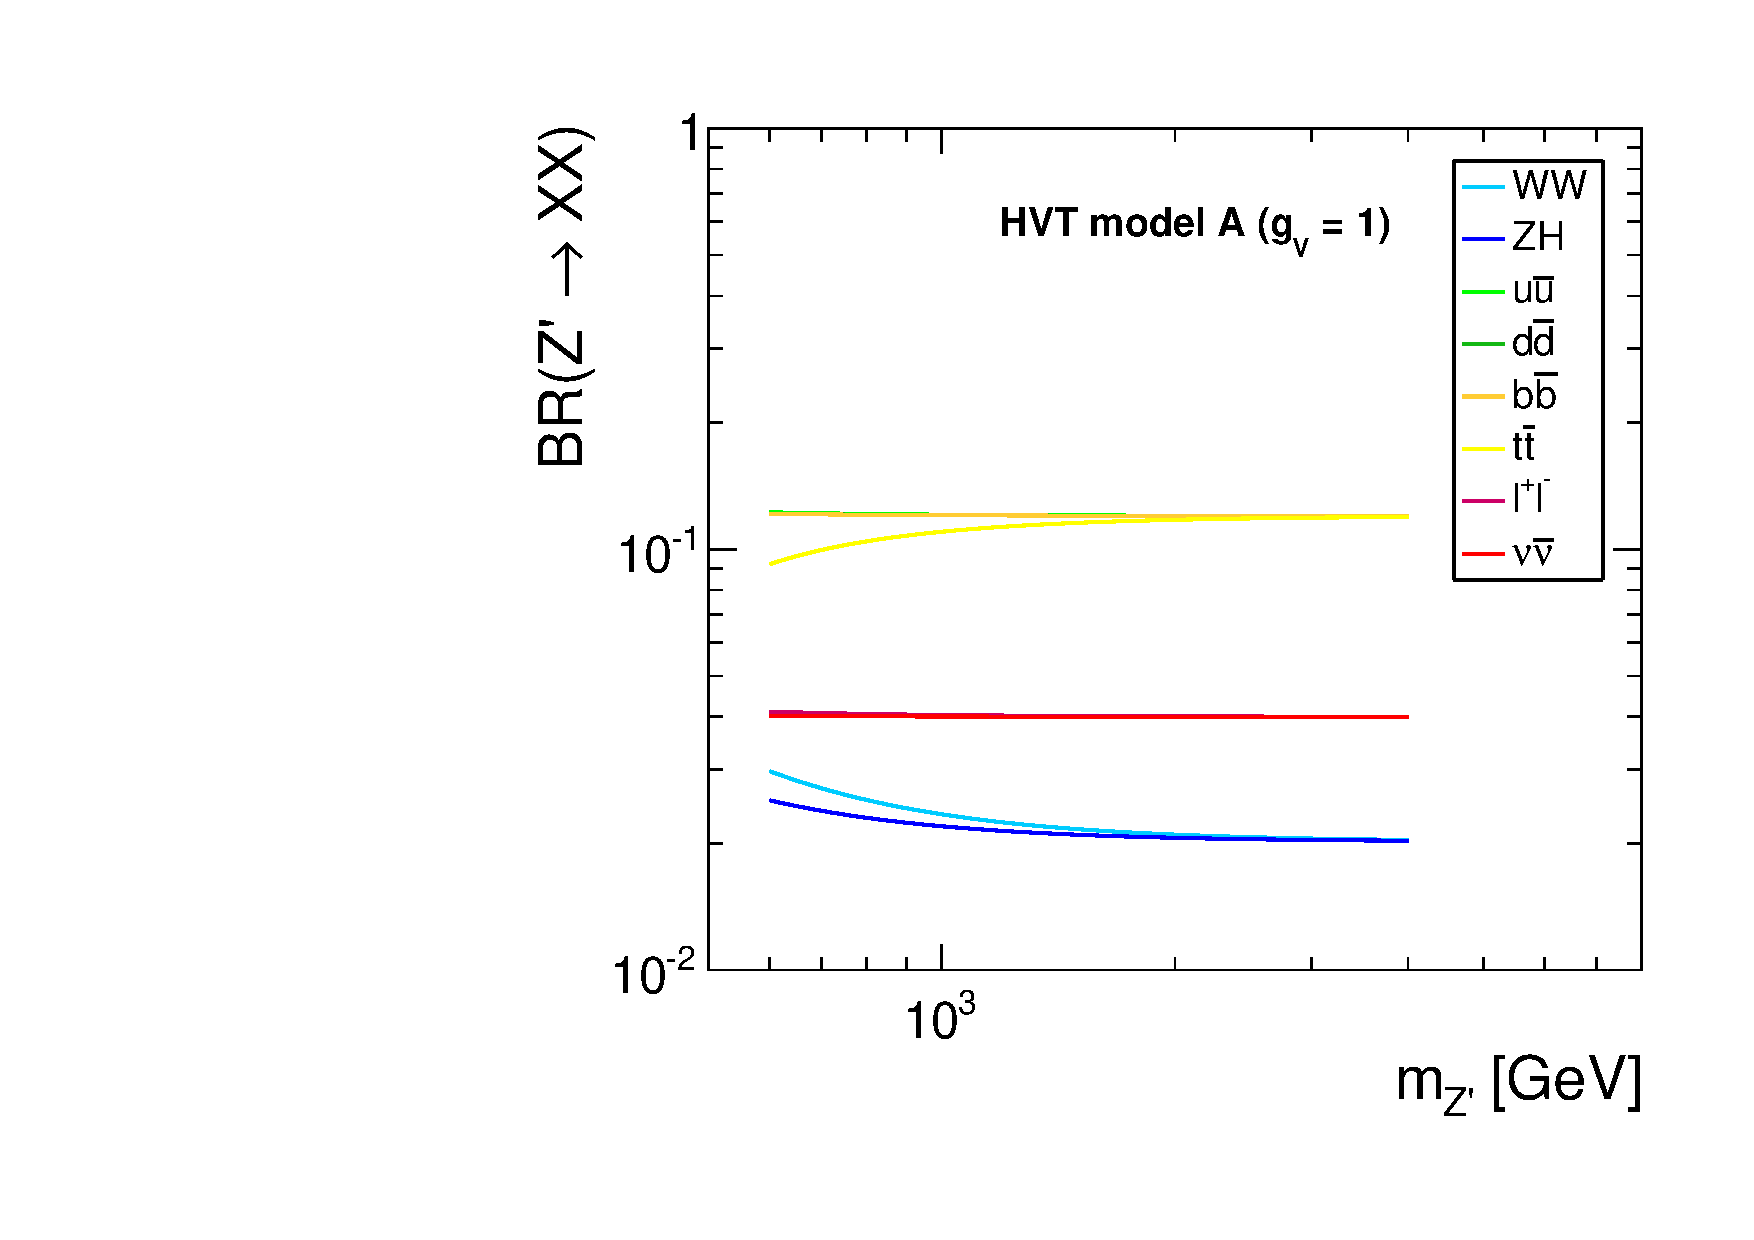
\includegraphics[width=0.45\textwidth]{\chtwo/brs-hvt-zprime-modelA.pdf}}
\subfigure[]{\label{fig:hvtBR_b}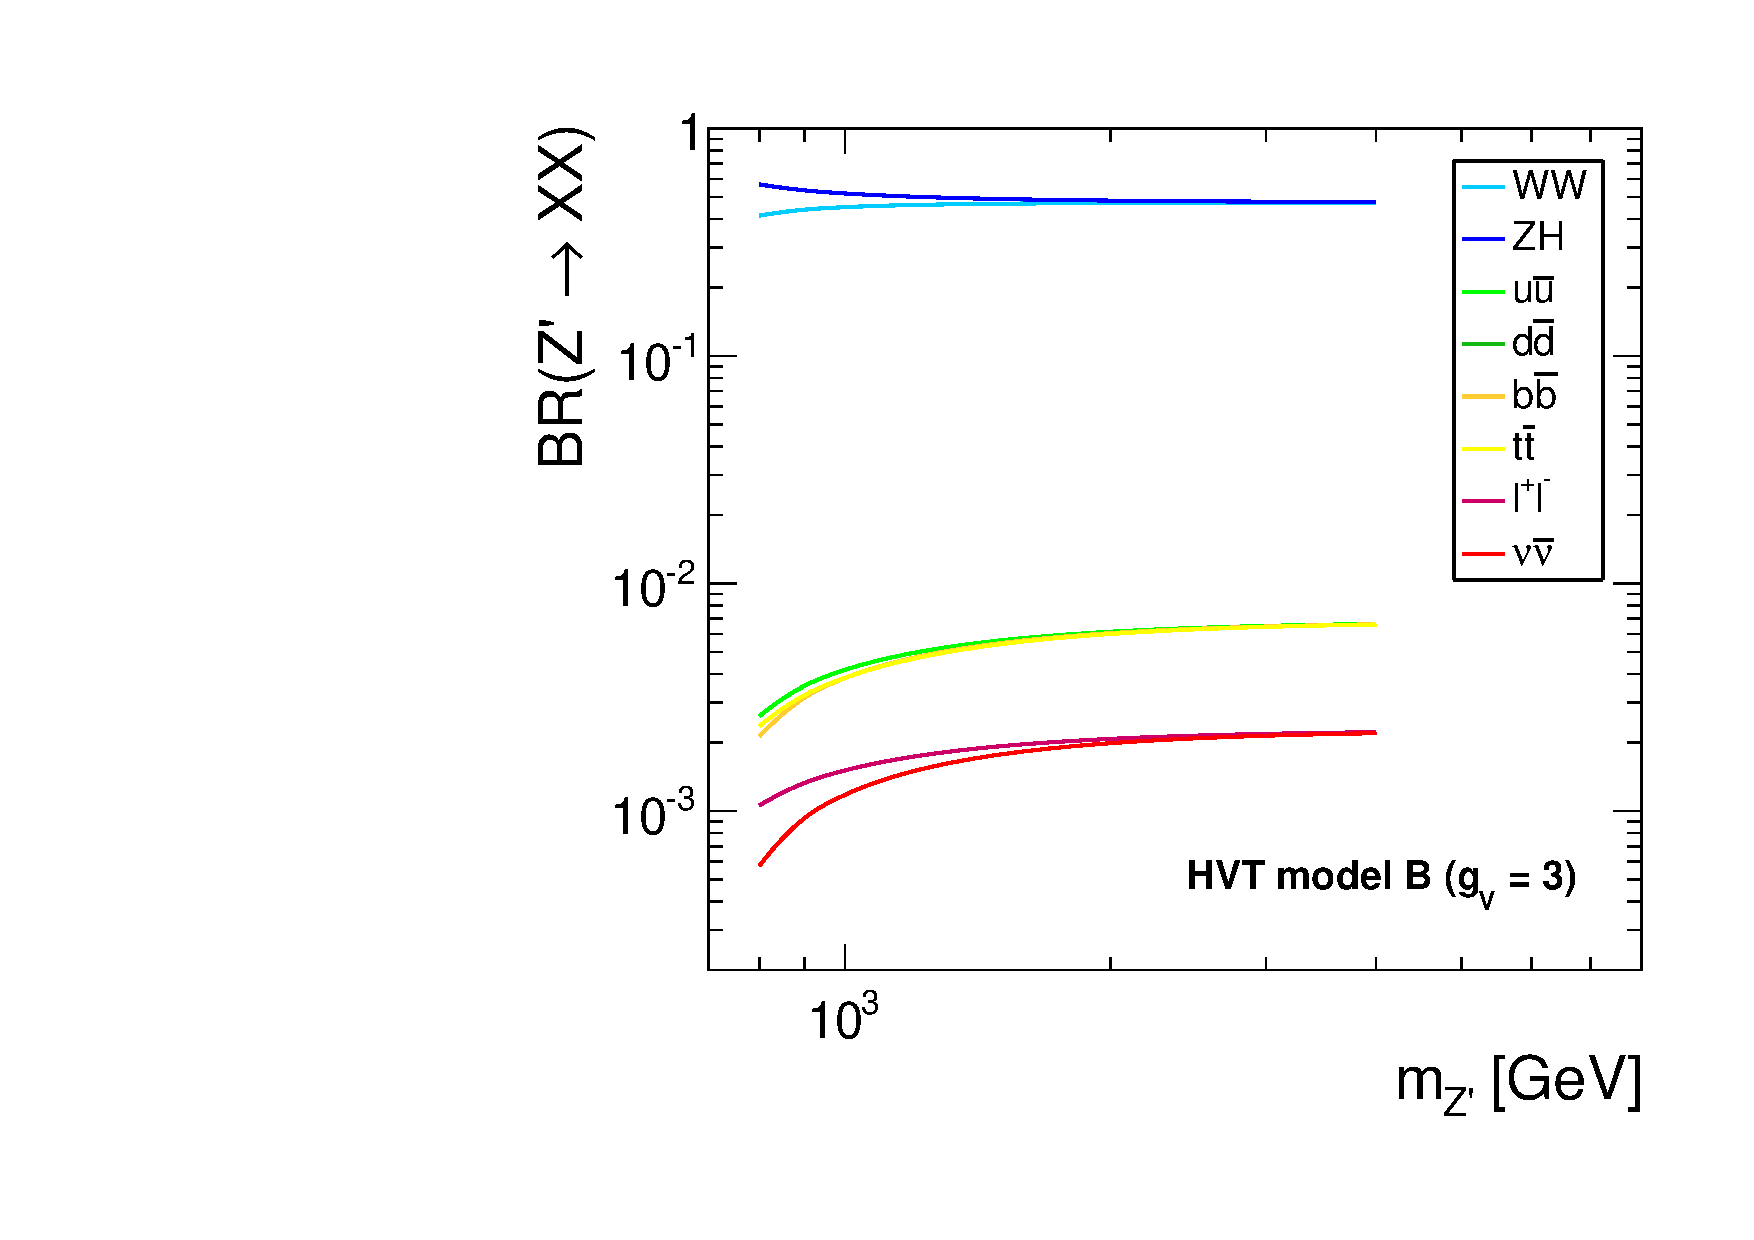
\includegraphics[width=0.45\textwidth]{\chtwo/brs-hvt-zprime-modelB.pdf}}
\caption{Branching fractions for the different decay modes of the neutral spin-1 resonance \Zpr ($V^0$) for the benchmarks (a) $\mathrm{A}_{g_V=1}$ (a) and (b) $\mathrm{B}_{g_V=3}$, as a function of the resonance mass.}
\label{fig:hvtBR}
\end{figure}

It has to be noted that the prediction of this simplified model are only valid for sufficiently narrow resonances.
In fact, several effects due to new physics, not included in this simplified framework, might contribute to the tail and radically change its prediction.
As a consequence, the results of an experimental search which is sensitive to the tail cannot be easily translated into bounds on the phenomenological parameter space.
  
